%%%%%%%%%%%%%%%%%%%%%%%%%%%%%%%%%%%%%%%%%
% Beamer Presentation
% LaTeX Template
% Version 1.0 (10/11/12)
%
%
% License:
% CC BY-NC-SA 3.0 (http://creativecommons.org/licenses/by-nc-sa/3.0/)
%
%%%%%%%%%%%%%%%%%%%%%%%%%%%%%%%%%%%%%%%%%

%----------------------------------------------------------------------------------------
%	PACKAGES AND THEMES
%----------------------------------------------------------------------------------------

\documentclass[aspectratio=1610]{beamer}
% aspectratio = 32,43,54,169,1610

\mode<presentation> {

% The Beamer class comes with a number of default slide themes
% which change the colors and layouts of slides. Below this is a list
% of all the themes, uncomment each in turn to see what they look like.



%\usetheme[numbering=none,progressbar=foot]{metropolis}
%\usetheme{default}
%\usetheme{AnnArbor}
%\usetheme{Antibes}
%\usetheme{Bergen}
%\usetheme{Berkeley}
%\usetheme{Berlin}
%\usetheme{Boadilla} % ----- simple
%\usetheme{CambridgeUS} %---- simple red
%\usetheme{Copenhagen}
%\usetheme{Darmstadt}
%\usetheme{Dresden}
%\usetheme{Frankfurt}
%\usetheme{Goettingen}
%\usetheme{Hannover}
%\usetheme{Ilmenau}
%\usetheme{JuanLesPins}
%\usetheme{Luebeck}
\usetheme{Madrid} % simple blue
%\usetheme{Malmoe}
%\usetheme{Marburg}
%\usetheme{Montpellier}
%\usetheme{PaloAlto}
%\usetheme{Pittsburgh}
%\usetheme{Rochester}
%\usetheme{Singapore}
%\usetheme{Szeged}
%\usetheme{Warsaw}

\setbeamertemplate{navigation symbols}{} 

%		For progress bar
%=======================================================
\setbeamercolor{progress bar progress}{use=progress bar,bg=progress bar.fg}
\defbeamertemplate{headline}{progress bar}{
  \dimen0=\paperwidth
  \multiply\dimen0 by \insertframenumber
  \divide\dimen0 by \inserttotalframenumber
  \edef\progressbarwidth{\the\dimen0}

  \leavevmode%
  \begin{beamercolorbox}[wd=\paperwidth,ht=0.7ex,dp=1ex]{progress bar}
    \begin{beamercolorbox}[wd=\progressbarwidth,ht=0.7ex,dp=1ex]{progress bar progress}
    \end{beamercolorbox}%
  \end{beamercolorbox}%
}

\setbeamertemplate{headline}[progress bar]
\setbeamercolor{progress bar}{fg=yellow2!100!black,bg=white!80!black}
%=======================================================



%		Custom Color Theme
%=======================================================
\definecolor{myblue}{RGB}{33,84,157}

%\setbeamercolor*{block title}{bg=myblue!20,fg=myblue}
%
\definecolor{yellow1}{RGB}{244,175,52}
\definecolor{blue1}{RGB}{114,195,232}
\definecolor{red1}{RGB}{234,63,38}

\definecolor{blue2}{RGB}{39,39,137}
\definecolor{yellow2}{RGB}{184,139,41}

\setbeamercolor{palette primary}   {use=structure,fg=white!100!white,bg=red1!100!white}
\setbeamercolor{palette secondary} {use=structure,fg=black!70!white,bg=blue1!100!white}
\setbeamercolor{palette tertiary}  {use=structure,fg=black!70!white,bg=yellow1!100!white}

\setbeamercolor{block title}{bg=green!20!black,fg=white}

\setbeamercolor{block body}{bg=green!30!black,fg=white}

%\setbeamercolor{section in head}{bg=green!30,fg=black}

\setbeamercolor{title}{bg=blue2!100,fg=white}		% For title background of title slide

\setbeamercolor{frametitle}{bg=blue2!100,fg=white}	% For header background of each slide	
%=======================================================


\setbeamercovered{transparent} % This is make slide elements transparent with \pause


% As well as themes, the Beamer class has a number of color themes
% for any slide theme. Uncomment each of these in turn to see how it
% changes the colors of your current slide theme.

%\usecolortheme{albatross}
%\usecolortheme{beaver}
%\usecolortheme{beetle}
%\usecolortheme{crane}
%\usecolortheme{dolphin}
%\usecolortheme{dove}
%\usecolortheme{fly}
%\usecolortheme{lily}
%\usecolortheme{orchid}
%\usecolortheme{rose}
%\usecolortheme{seagull}
%\usecolortheme{seahorse}
%\usecolortheme{whale}
%\usecolortheme{wolverine}

%\setbeamertemplate{footline} % To remove the footer line in all slides uncomment this line
%\setbeamertemplate{footline}[page number] % To replace the footer line in all slides with a simple slide count uncomment this line

%\setbeamertemplate{navigation symbols}{} % To remove the navigation symbols from the bottom of all slides uncomment this line
}

\usepackage{lmodern}
\usepackage{graphicx} % Allows including images
\usepackage{booktabs} % Allows the use of \toprule, \midrule and \bottomrule in tables
%\usepackage[dvipsnames]{xcolor}
\usepackage{tikz}

%----------------------------------------------------------------------------------------
%	TITLE PAGE
%----------------------------------------------------------------------------------------

\title[Research Scholar Day]{Elliptic flow analysis with non-hydro mode in viscous hydrodynamics } % The short title appears at the bottom of every slide, the full title is only on the title page

\titlegraphic{

\includegraphics[scale=0.055]{figs/bits_pilani_logo.png}%
}


\author{ Nikhil Hatwar } % Your name
\institute[] % Your institution as it will appear on the bottom of every slide, may be shorthand to save space
{
 Supervisor : Prof. Madhukar Mishra\\~\\
 DAC Members : Prof. Tapomoy Guha Sarkar and Prof. Navin Singh\\

\medskip
{\large Physics Department, Birla Institute of Technology and Science, Pilani } \\ % Your institution for the title 
\medskip
{\LARGE Research Scholar Day}\\
}
\date{$26^{th}$ March 2022}
\vspace*{-9mm}










\begin{document}
%------------------------------------------------
\begin{frame}
\titlepage % Print the title page as the first slide
\end{frame}



%----------------------------------------------------------------------------------------
%	PRESENTATION SLIDES
%----------------------------------------------------------------------------------------







%------------------------------------------------
 % Sections can be created in order to organize your presentation into discrete blocks, all sections and subsections are automatically printed in the table of contents as an overview of the talk
%------------------------------------------------

 % A subsection can be created just before a set of slides with a common theme to further break down your presentation into chunks

\begin{frame}
\frametitle{Quantum Chromodynamics} 

\begin{itemize}

\item Non-abelian gauge theory of strong interactions.

\begin{block}{QCD lagrangian}
\begin{equation}
\mathcal{L}_\mathrm{QCD} = \bar{\psi}_i \,  i \, \gamma^\mu \left( \partial_\mu \delta_{ij} - i g \left( T_a \right)_{ij} \mathcal{A}^a_\mu \right) \psi_j  - m\, \bar{\psi}_i  \psi_i - \frac{1}{4}G^a_{\mu \nu} G^{\mu \nu}_a
\end{equation}	
\end{block}		
	
where, \\
	\hspace*{20mm}		$\gamma$  -- Dirac matrices\\
	\hspace*{20mm}		$\lambda_a$  -- Gell-Mann matrices(a = 1 \ldots 8)\\
	\hspace*{20mm}		$G^a_{\mu \nu}$ -- gauge invariant gluon field strength tensor\\
	\hspace*{20mm}		$\mathcal{A}^a_\mu$  -- 8 Gluon fields\\
	\hspace*{21mm}		$\psi_i$  -- Quark field\\

\item Color charge is conserved. This local symmetry is governed by SU(3) guage group.

\item Strong interaction does not discriminate between flavors -- approximate flavor symmetry -- also follows SU(3) group.

\item Quarks are never observed in free state below Hagedorn temperature -- Color Confinement 

%\item Quite well tested in perturbative regime.  

\end{itemize}

\end{frame}

%------------------------------------------------

\begin{frame}
\vspace*{-6mm}

\frametitle{Open questions in QCD}

\begin{columns}
% Column 1
\begin{column}{0.6\textwidth}
\textbf{Mapping out QCD phase diagram:}\\

What are the phases of strongly interacting matter? Location of critical point ? \\~\\
What are the equilibrium and transport properties of quark-gluon plasma ? \\~\\

\textbf{Onset of deconfinement}: \\
 as a function of temperature and chemical potentials? \\
 as a function of relativistic heavy-ion collision energy and system size?\\~\\~\\
\textit{Eur. Phys. J. A 56:267 (2020)}\\
 \textit{Rep. Prog. Phys. 84 056301 (2021)}\\
\end{column}
% Column 2    
\begin{column}{0.4\textwidth}
    \begin{figure}
    \centering
    
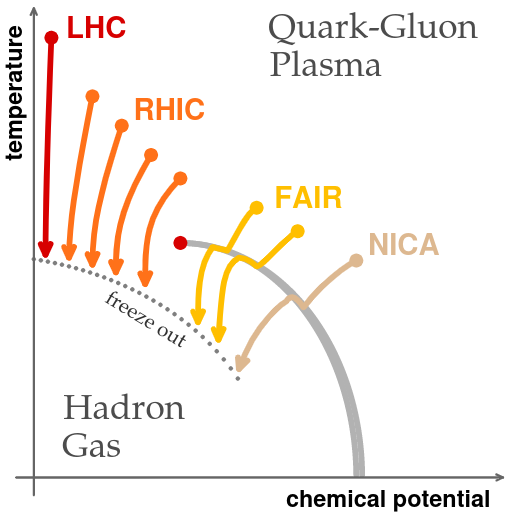
\includegraphics[scale=0.2]{figs/QCD_Phase_diagram_2021_Gelis.png} \\
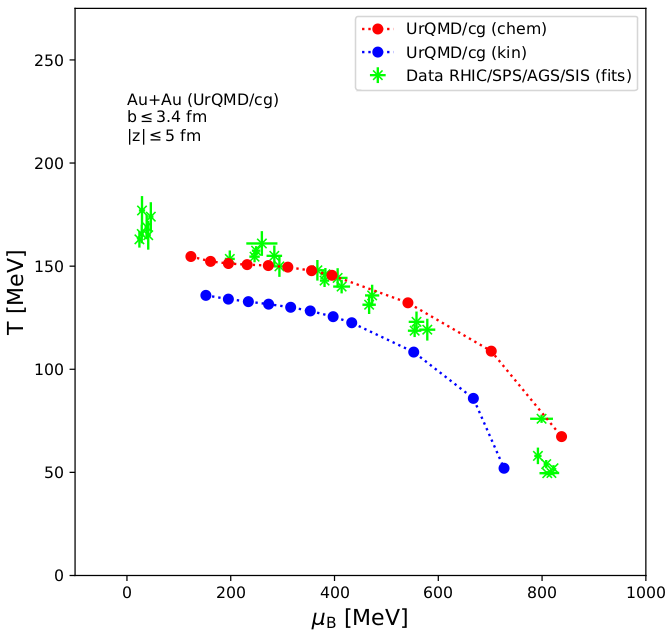
\includegraphics[scale=0.2]{figs/abc.png} 
 \end{figure}
\end{column}
\end{columns}

\end{frame}





%------------------------------------------------

\begin{frame}
\frametitle{Müller, Israel and Stewart (MIS) $2^{nd}$ order Hydrodynamics (1/2)}
%\vspace*{-9mm}

\begin{itemize}

\item Expt data provide strong support for hydrodynamics as the appropriate effective theory for RHIC.

%\item Hydrodynamics is the collective dynamical evolution of a suitably sized bulk medium adhering to the system's symmetries. 

\item Relativistic conservation laws: , $\partial_{\mu} T^{\mu\nu}=0$ and $\partial_{\mu} N^\mu=0$. 


\item The local values of temperature, $\mathcal{T}(x)$, fluid velocity, $u_\mu(x)$ and chemical potential, $\mu(x)$ are the chosen hydrodynamic variables. 

\begin{block}{Energy-momentum tensor decomposition}
\begin{equation}
T^{\mu\nu}=\epsilon u^\mu u^\nu + P\Delta^{\mu\nu}+ ( w^\mu u^\nu + w^\nu u^\mu) + \Pi^{\mu\nu}
\end{equation}

\end{block}

\hspace*{10mm}		$w^\mu$ -- Transverse vector coefficient\\
\hspace*{10mm}		$\Delta^{\mu\nu} \equiv ( g^{\mu\nu} +  u^\mu u^\nu)$ -- Projector operator orthogonal to the fluid velocity, $u^\mu$\\
\hspace*{10mm}		$\epsilon$ --  Energy density  \\
\hspace*{10mm}		$P$ --  Pressure\\
\hspace*{10mm}		$\Pi^{\mu\nu} = \pi^{\mu\nu} +  \Delta^{\mu\nu}\Pi$  --  Tensor introduced to account for the dissipative effects\\
\hspace*{10mm}		$\Pi$ -- Bulk pressure\\
\hspace*{10mm}		$\pi^{\mu\nu}$ -- Shear stress tensor

\end{itemize}
\textit{Inter. Journal of Modern Physics, 19 1 pp.1-53 (2010)} \\
%\textit{Zeitschrift für Physik 198, 329 (1967).} \\
\end{frame}

%------------------------------------------------



\begin{frame}
\frametitle{Müller, Israel and Stewart (MIS) $2^{nd}$ order Hydrodynamics (2/2)}
%\vspace*{-9mm}


%\item We have used ECHO-QGP hydrodynamics with lattice QCD Equation of State by Wuppertal-Budapest collaboration. \textit{Journal of High Energy Physics 2010, 1 (2010)}

\begin{block}{Shear stress tensor for MIS hydro}
\begin{equation}
\pi^{\mu\nu} = -\eta \Bigl( 2\sigma^{\mu\nu} + \frac{4}{3} \frac{\tau_\pi}{\eta} d_\mu u^\mu \pi^{\mu\nu} + \frac{\tau_\pi}{\eta} \Delta^\mu_\alpha \Delta^\nu_\beta D \pi^{\alpha\beta}  \nonumber +  \frac{\lambda_0}{\eta} \tau_\pi ( \pi^{\mu\lambda} \Omega^\nu_\lambda + \pi^{\nu\lambda} \Omega^\mu_\lambda ) \Bigr)
\end{equation}
\end{block}

Here, $\lambda_0$ is a scalar coefficient and $\Omega$ is a traceless, anti-symmetric, transverse vorticity tensor. 
$d_\mu$ is the covariant derivative,  $D = u^\mu d_\mu$, is the comoving time derivative.

\begin{block}{Bulk pressure for MIS hydro}
\begin{equation}
\Pi = -\zeta \left( d_\mu u^\mu + \frac{\tau_\Pi}{\zeta} u^\alpha d_\alpha \Pi + \frac{4}{3} \frac{\tau_\Pi}{\zeta} \Pi \; d_\mu u^\mu \right)
\end{equation}
\end{block}

The value of $\tau_\Pi$, $\lambda_0$, $\tau_\pi$, $\eta$, $\zeta$ has to be provided for solving the above two equations.\\~\\

\textbf{$\tau_\Pi$ and $\tau_\pi$ are the bulk viscosity and shear relaxation times, representing how quickly the above $2^{nd}$ order form of $\Pi$ and $\pi^{\mu\nu}$ relaxes to its leading-order forms.} \\~\\

\textit{Eur. Phys. J. C (2013) 73:2524} \\

\end{frame}


%------------------------------------------------


\begin{frame}
\frametitle{Non-hydro modes}
%\vspace*{-9mm}

If the dynamics show quasi-universality at large time scale, one can derive hydrodynamics from it.


\begin{block}{Energy momentum tensor for microscopic theory in a non-equilibrium state}
\begin{equation}
T^{\mu\nu} =  \langle \hat{T^{\mu\nu}} \rangle_{eq} + \delta \langle \hat{ T^{\mu\nu}} \rangle
\end{equation}
\end{block}

where,\\
\hspace*{10mm}  first term -- equilibrium values of $T^{\mu\nu}$ \\
\hspace*{10mm}  second term -- deviations from that equilibrium value. \\~\\

This second term is given under linear response theory in terms of the retarded $2-$point correlator of $T^{\mu\nu}$. \\~\\

This correlator when expressed in the Fourier space, has singularities in $\omega$-plane. This is the \textbf{quasinormal mode}.\\~\\

\textit{2018 Rep. Prog. Phys. 81 046001}

\end{frame}

%------------------------------------------------

\begin{frame}
\frametitle{Quasinormal modes}
\begin{block}{Quasinormal frequency}
\begin{equation}
{\LARGE \omega = \omega_h + i \; \omega_{nh} }
\end{equation}
\end{block}
where, \\

\hspace*{10mm}	$\omega_h$ -- excitation frequency for equilibrium plasma and is called a hydrodynamic mode. \\

\hspace*{10mm}	$\omega_{nh}$ -- transient mode or non-hydrodynamic mode frequency and is associated with the dissipative effects.  \\~\\

{\Large \textbf{Transient mode disrupts  hydrodynamization and is controlled with the relaxation time parameter.}}
\end{frame}
%------------------------------------------------




\begin{frame}
\frametitle{Initial conditions for hydrodynamics}
%\vspace*{-9mm}


\hspace*{6mm} {\Large \textbf{IPGlasma}}


\begin{itemize}

\item Effective theory wavefunction of the high energy nuclei/hadron -- \textbf{Color Glass Condensate}.\\

\item The distribution of nucleons acts as sources of initial state fluctuations.\\

\item Gaussian sampled color charges act as a source for gluon fields which are evolved using classical Yang-Mills equations.\\


\textit{PRC 86, 034908 (2012)}, \textit{PRL 108, 252301 (2012)} \\~\\



 {\Large \textbf{Glauber}} 


\item Glauber assumes nucleons being distributed with Wood-Saxon profile and having independent linear trajectories. 

\item Wood-Saxon distribution has a smooth plateau for nucleus which decays softly towards the edges.

%\item When two nuclei collide at some impact parameter, the number of participant's nucleon density is calculated using a simple relation with the inelastic nucleon-nucleon cross section as input.

\textit{Ann.Rev.Nucl.Part.Sci. 57 (2007) 205-243}

\end{itemize}
\end{frame}

%------------------------------------------------

\begin{frame}

\frametitle{Initial energy density plots}

\begin{figure}
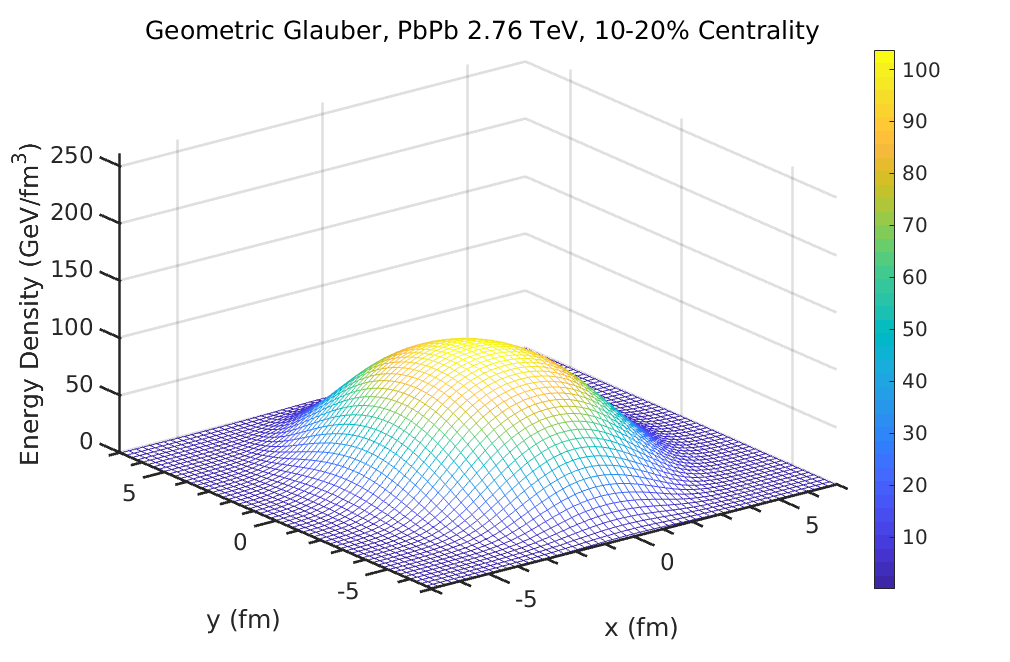
\includegraphics[scale=0.28]{figs/3DGeometric.png}
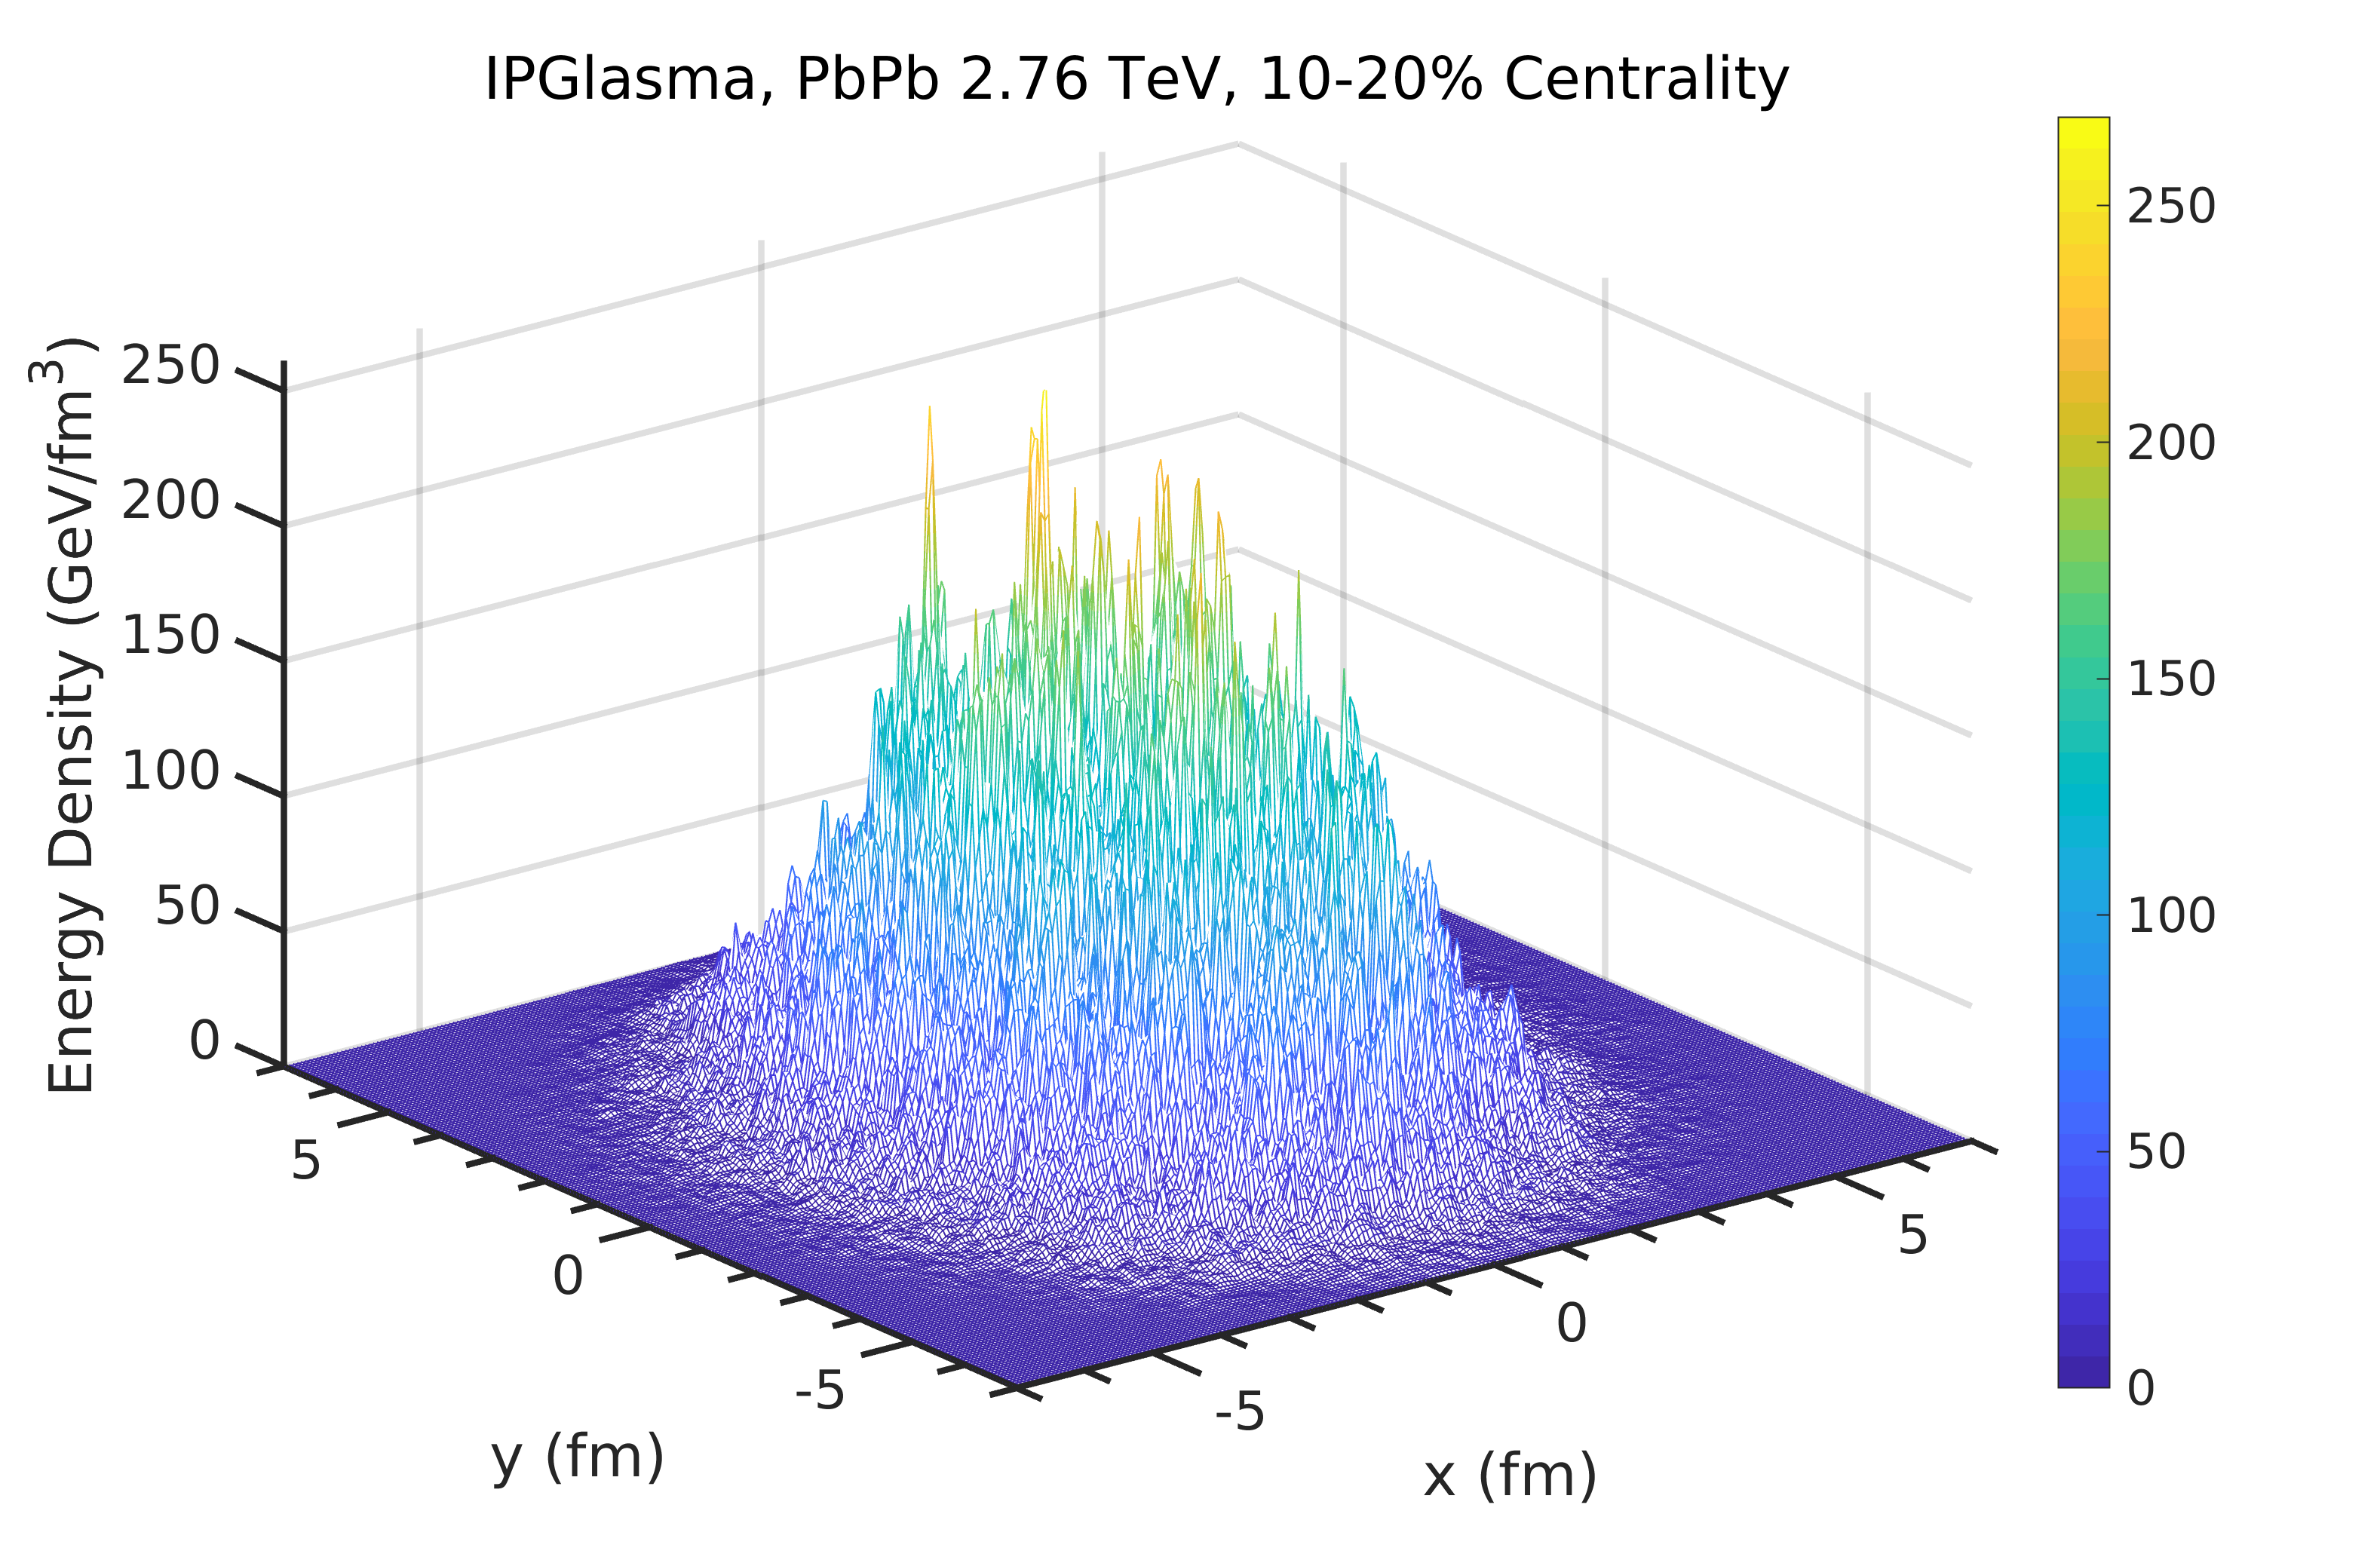
\includegraphics[scale=0.28]{figs/IPGlasma.png}
\end{figure}

\begin{itemize}
\item Notice IPGlasma profile being extremely jagged and spiky, whereas Glauber initial condition is quite smooth. 

\item Two extreme limits of the initial state fluctuation viz. very high and very low spatial eccentricities.

\end{itemize}
\end{frame}



%------------------------------------------------

\begin{frame}

\frametitle{Pion $p_T$ spectra plots}

\begin{figure}
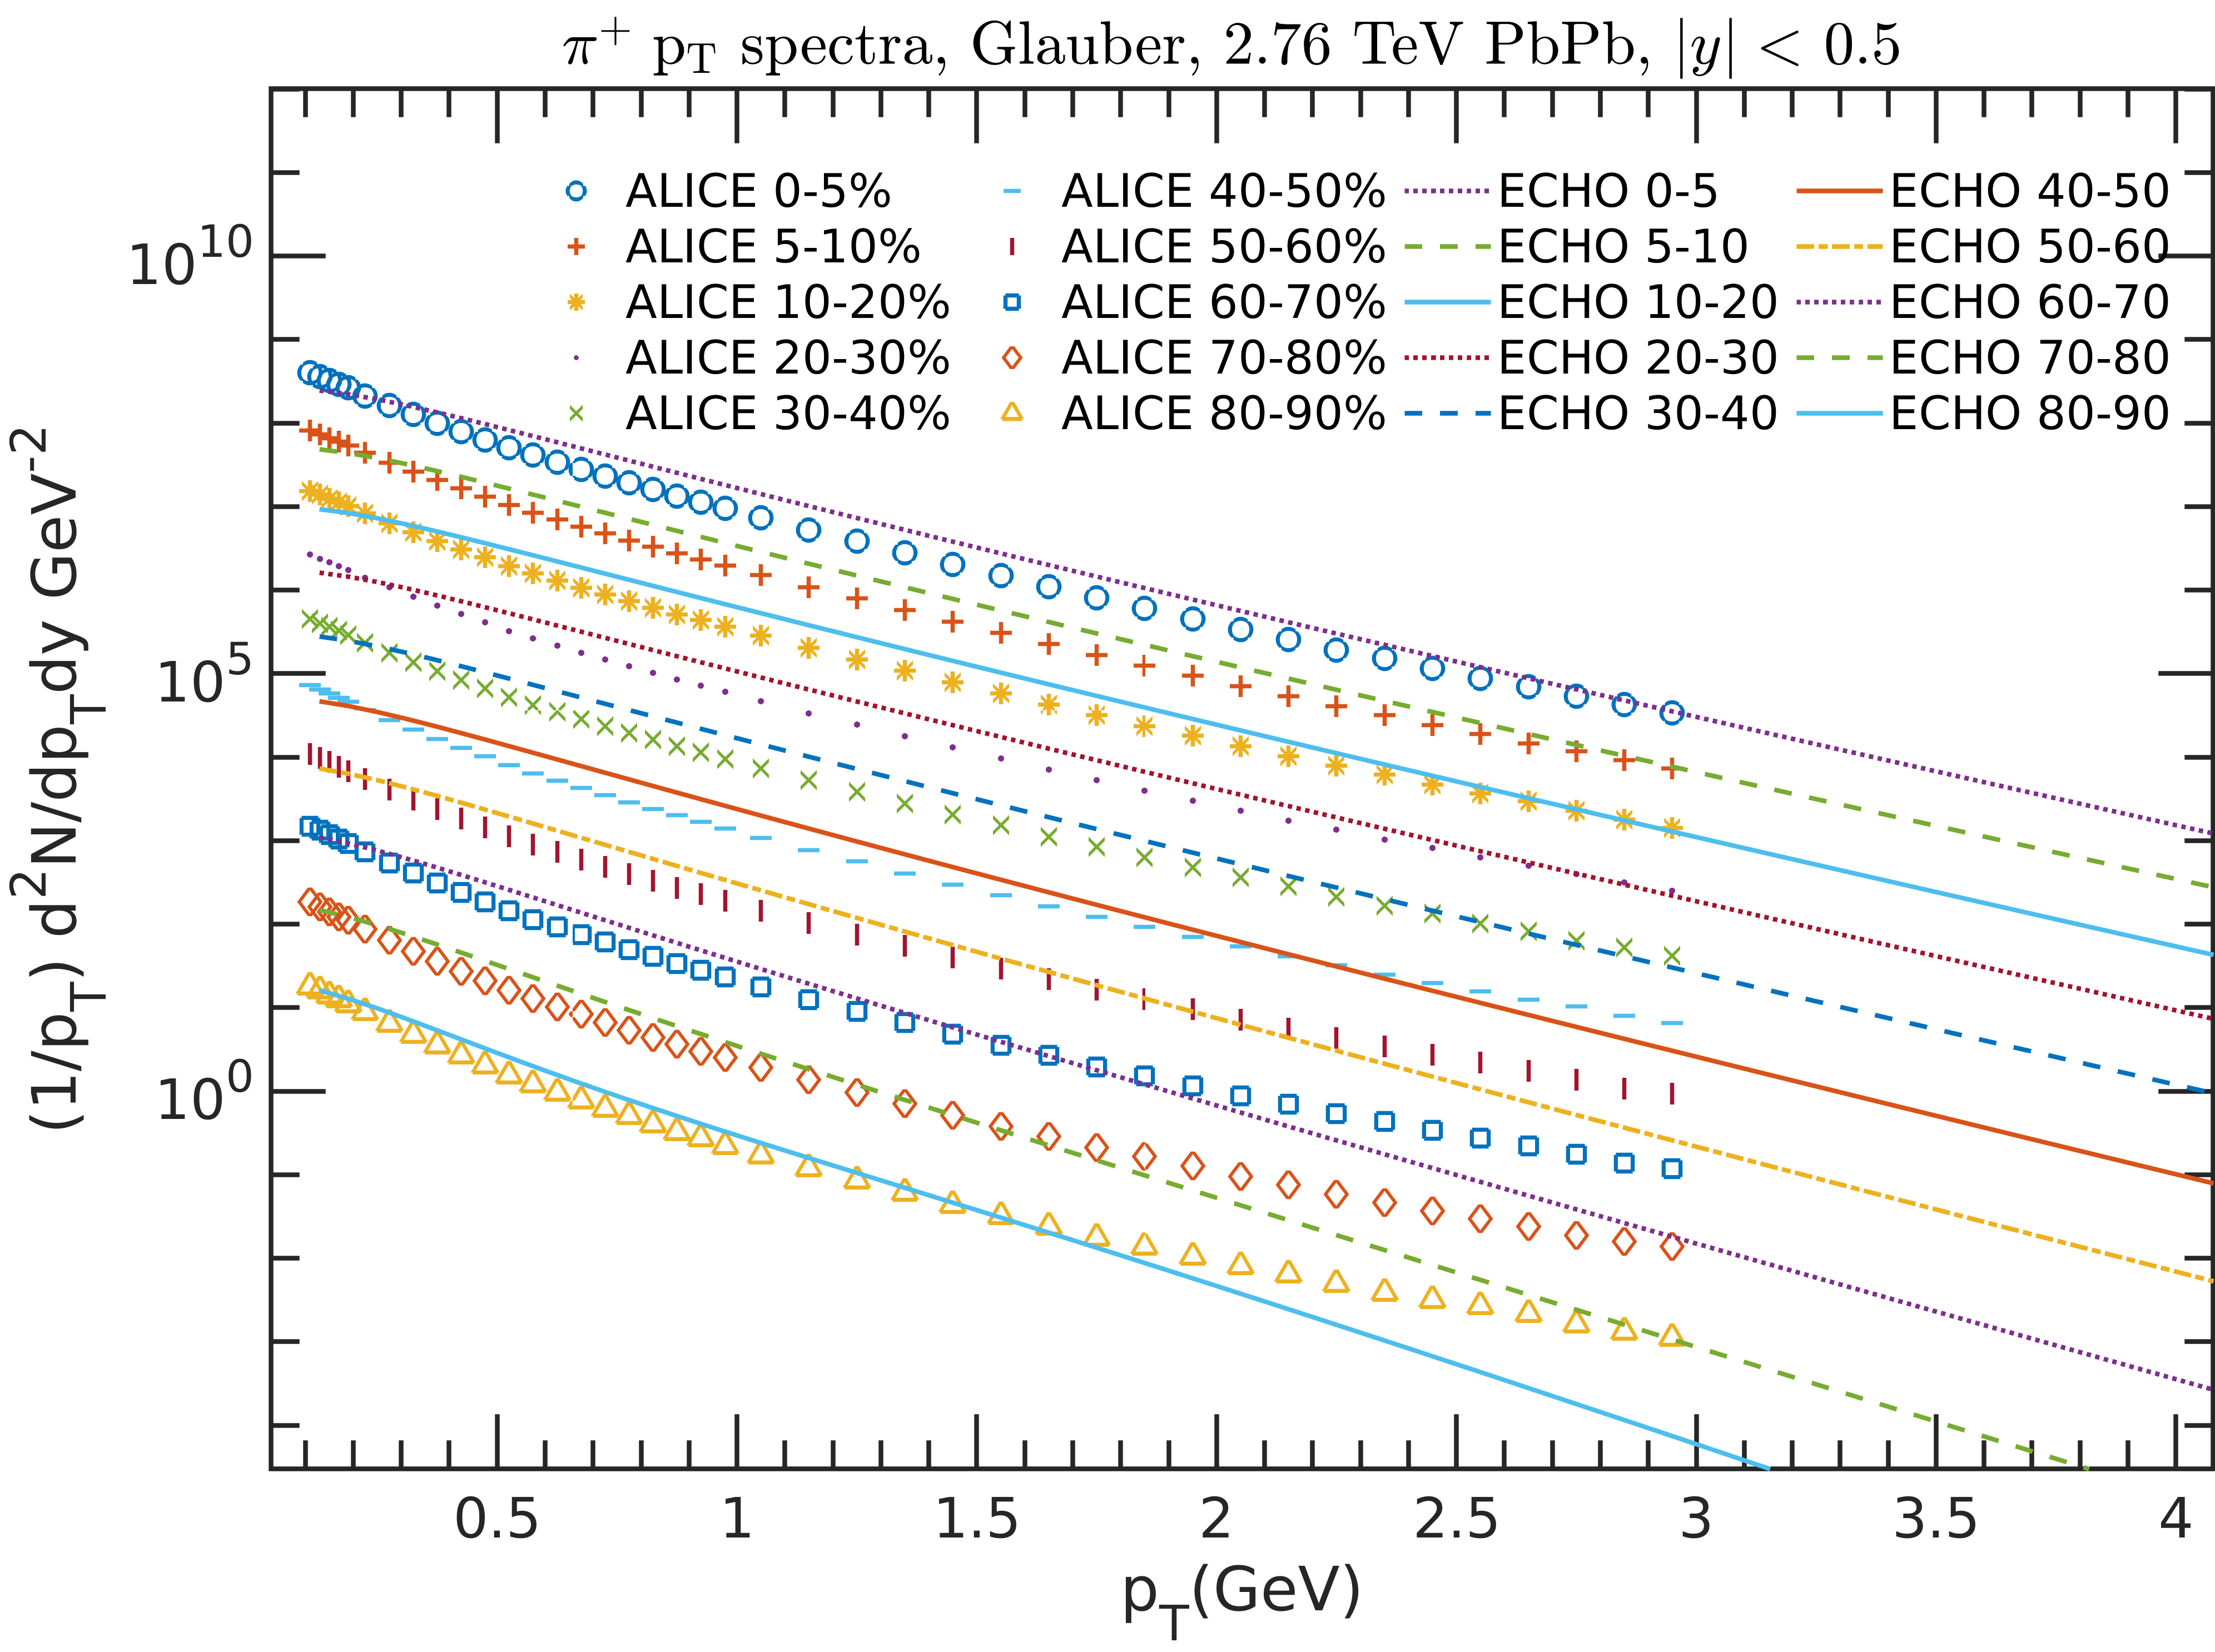
\includegraphics[scale=0.22]{figs/pT-spec_3Dgeometric.png}
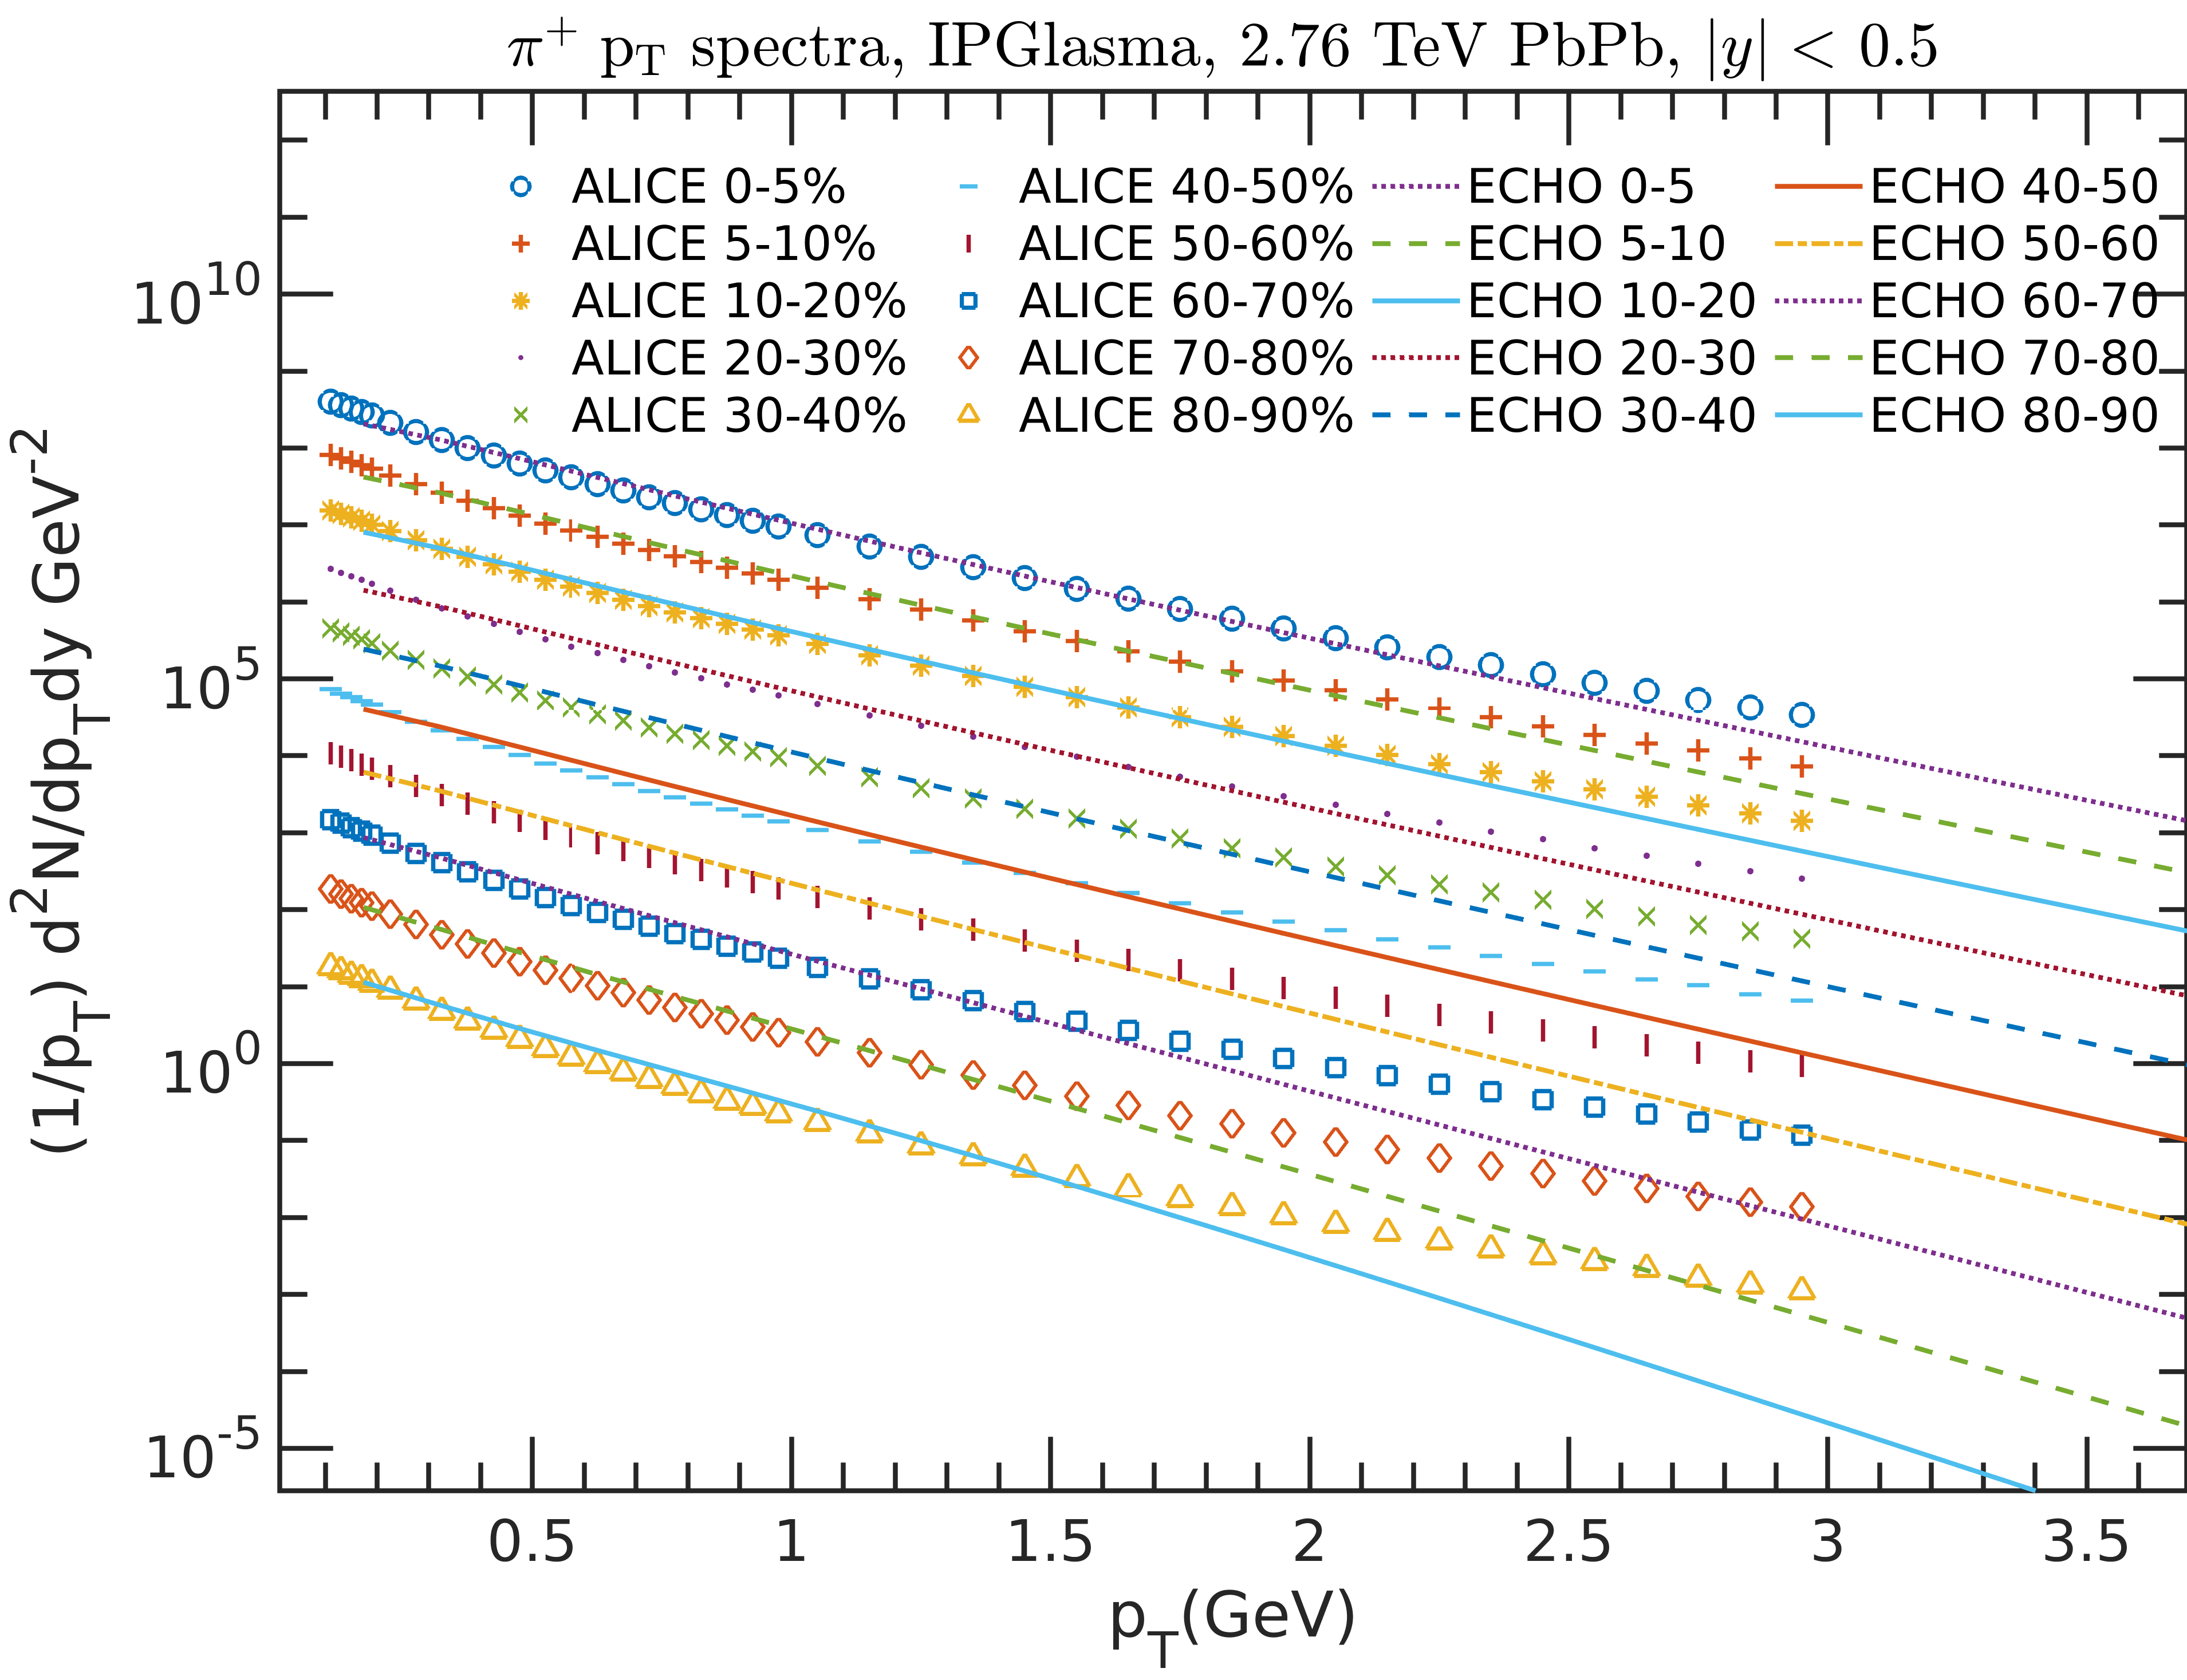
\includegraphics[scale=0.22]{figs/pT-spec_IPGlasma.png}
\end{figure}

\begin{itemize}
\item Slightly better match for IPGlasma than Glauber. 

\item Spectra comply to experimental values only in low $p_T$ regime, where the hydrodynamic mode operates.

\textit{Phys. Rev. C 93, 034913 (2016)}

\end{itemize}


\end{frame}


%------------------------------------------------







\begin{frame}
\frametitle{Thermodynamic eccentricities}

{ \Large Spacial eccentricity:}

\begin{equation}
e_c =  \frac{\int dx \; dy\;[ ( x-x_0 )^2 - (y-y_0)^2 ] }{\int dx \; dy\; [ ( x-x_0 )^2 + (y-y_0)^2 ]}
\end{equation}\\~\\



{ \Large Momentum eccentricity:}
\begin{equation}
e_p\equiv  \frac{\int d^2x_\perp ( T^{xx}-T^{yy} )}{\int d^2x_\perp ( T^{xx}+T^{yy} )}
\end{equation}\\
\begin{equation}
e_p \equiv \frac{\int d^2x_\perp (\epsilon+P) \left(u^x u^x-u^y u^y\right) + \pi^{xx} + \pi^{yy}}{\int d^2x_\perp [ (\epsilon+P) \left(u^x u^x+u^y u^y\right)+2P + \pi^{xx} + \pi^{yy}]}
\end{equation}

($\pi^{xx} + \pi^{yy}$) term has been added as viscous corrections to ideal hydrodynamic momentum eccentricity.\\
\textit{Eur. Phys. J. C (2015) 75 429}
\end{frame}



%------------------------------------------------



\begin{frame}
\vspace*{-3mm}
\frametitle{Eccentricity during hydrodynamic evolution}

\begin{columns}
% Column 1
\begin{column}{0.4\textwidth}

\begin{itemize}
\item $e_c$ vaguely represents initial state fluctuations.  

\item  Initial state fluctuations leads to momentum anisotropy in the system, which translates to larger collective flow. 

\item  Notice the larger $e_c$ for IPGlasma initial condition. 

\item Also notice larger change in $e_p$ due to increase in relaxation time. 

\end{itemize}
     
\end{column}
% Column 2    
\begin{column}{0.6\textwidth}
    \begin{figure}
    \centering
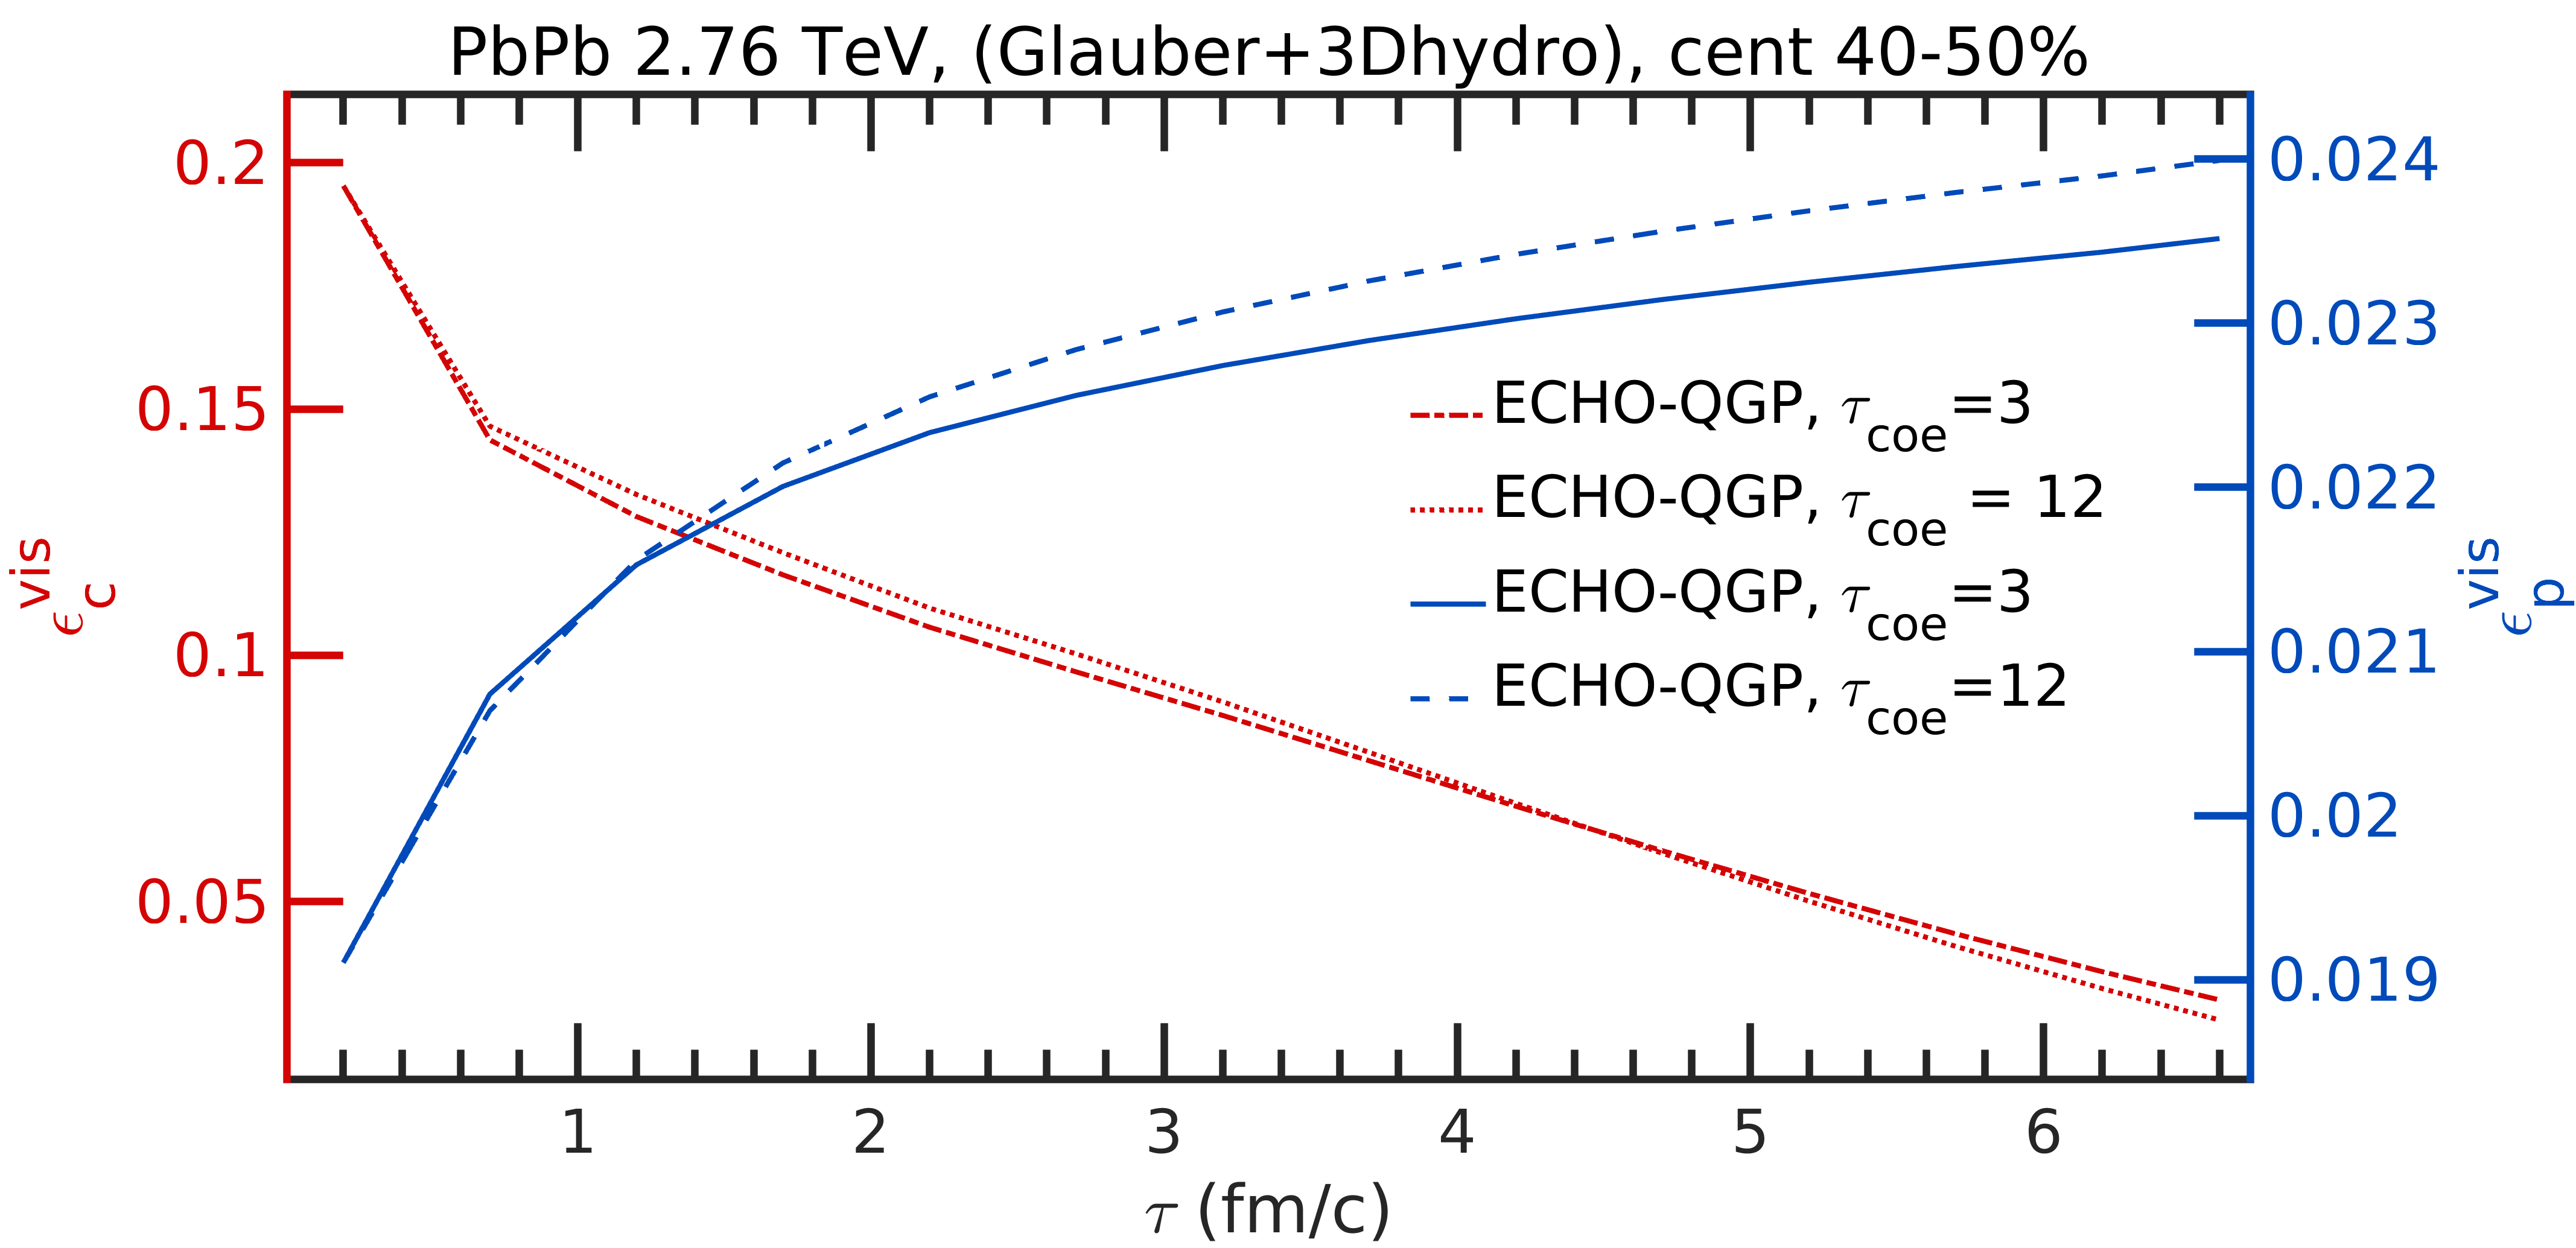
\includegraphics[scale=0.23]{figs/EC_EP_3Dgeometric.png}
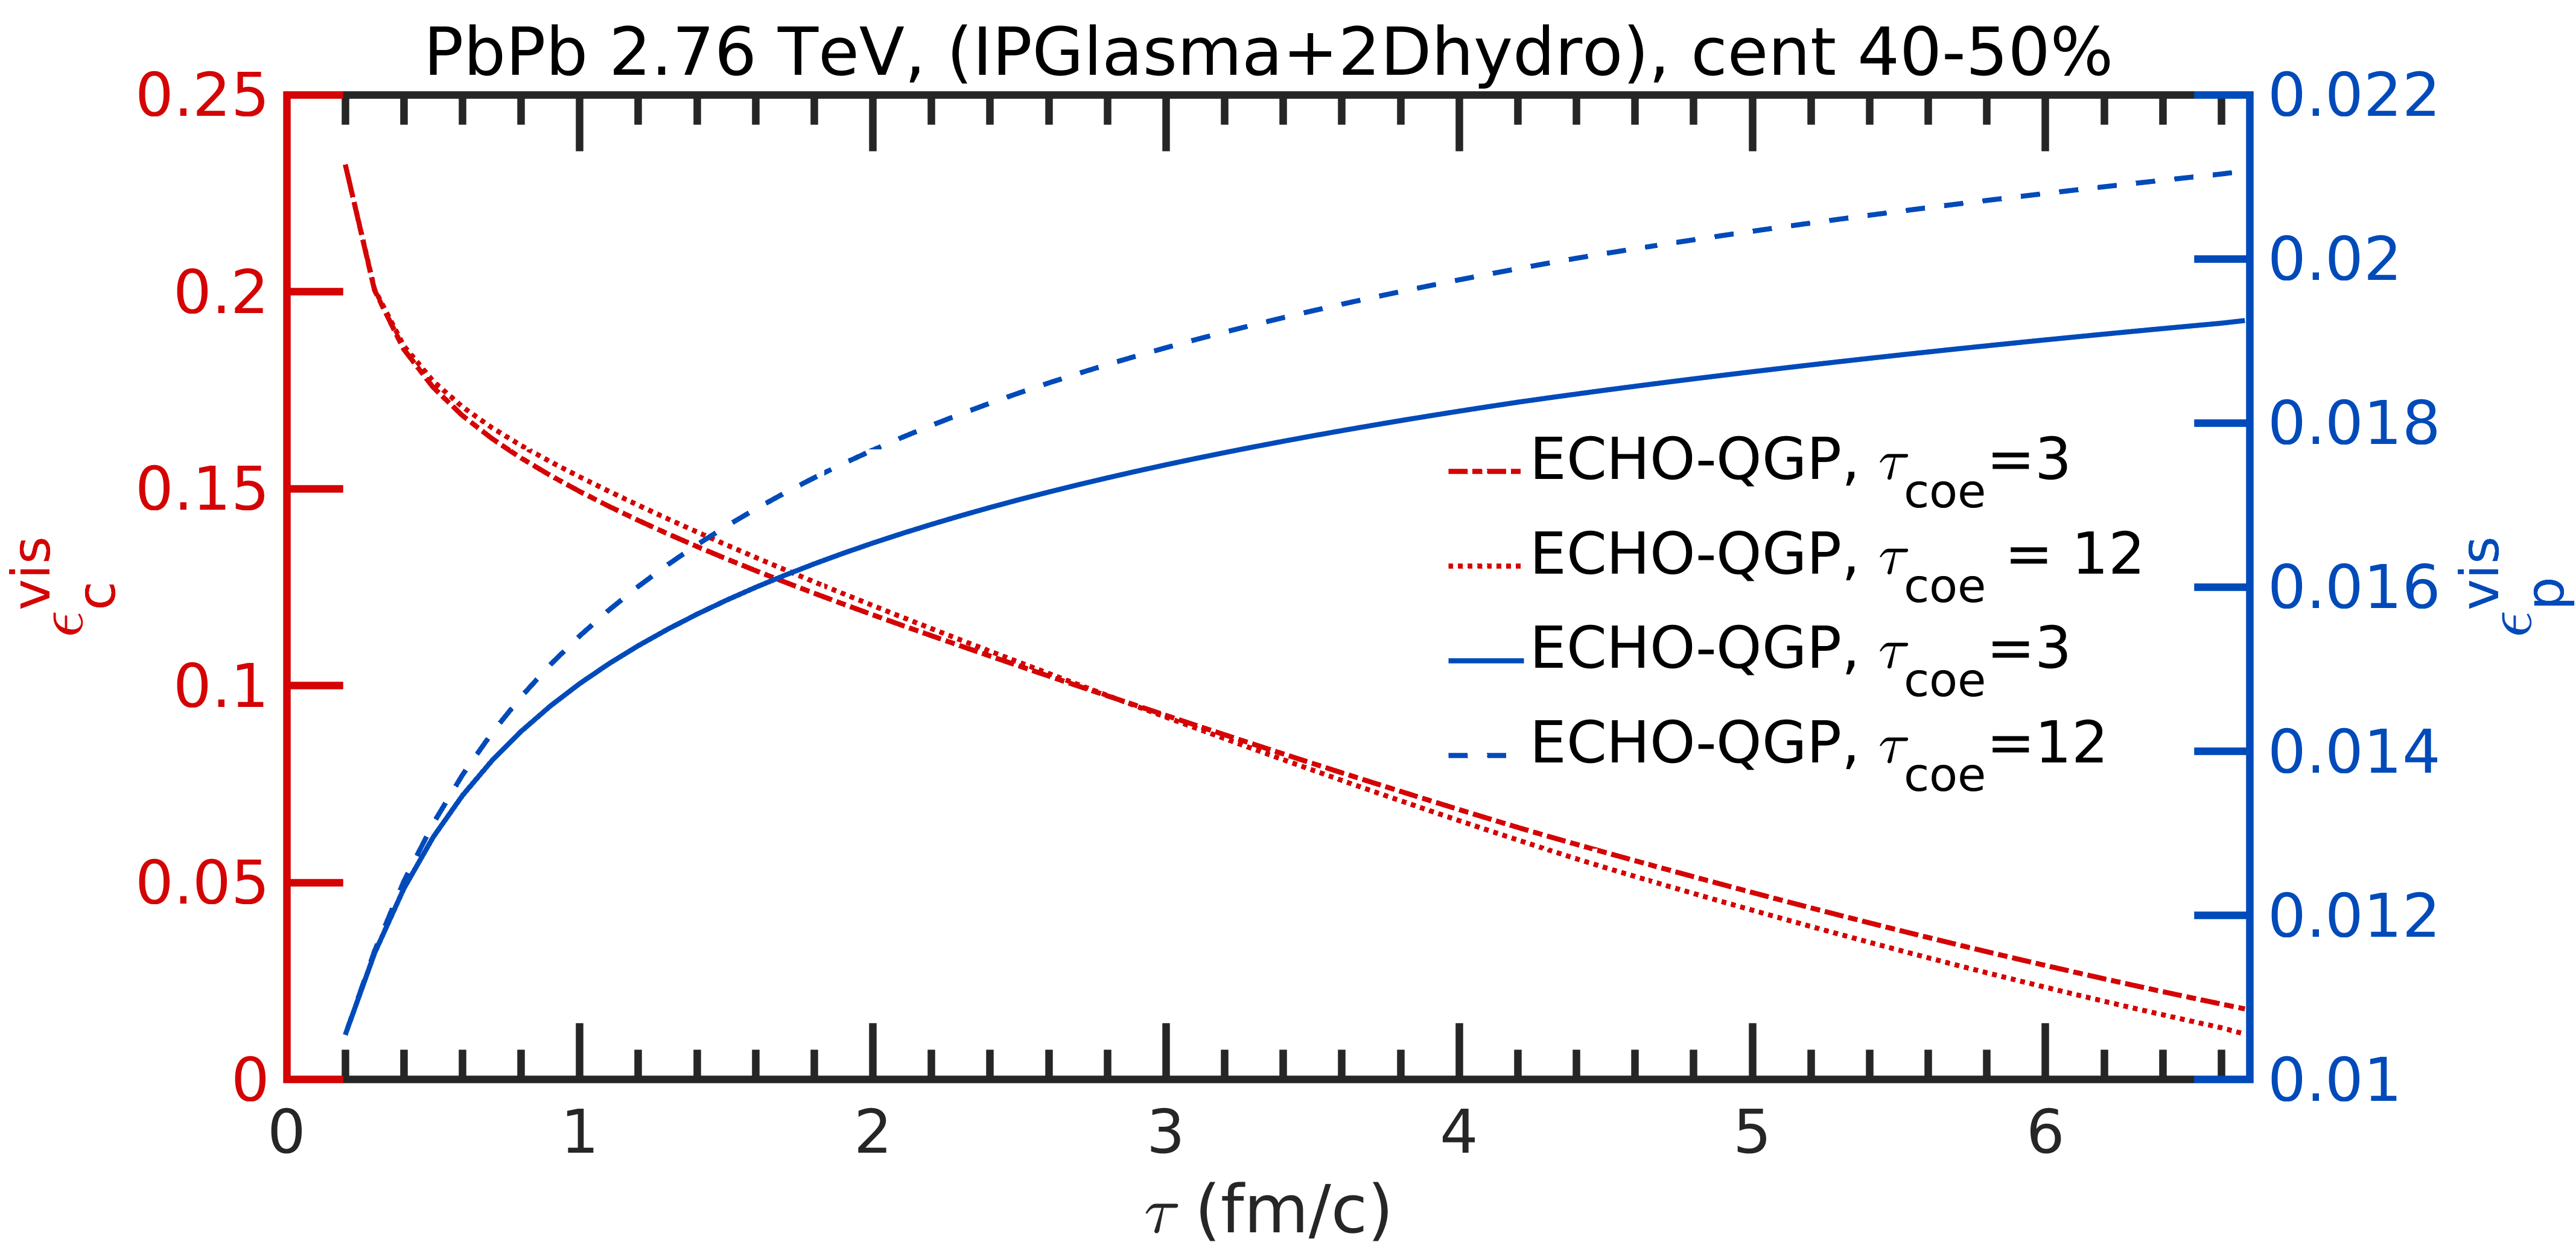
\includegraphics[scale=0.23]{figs/EP_EC_ipglasma.png}
    \end{figure}
\end{column}
\end{columns}

\begin{figure}

\end{figure}
\end{frame}




%------------------------------------------------



\begin{frame}

\frametitle{Effect of non-hydro mode in Glauber elliptic flow}

\begin{figure}
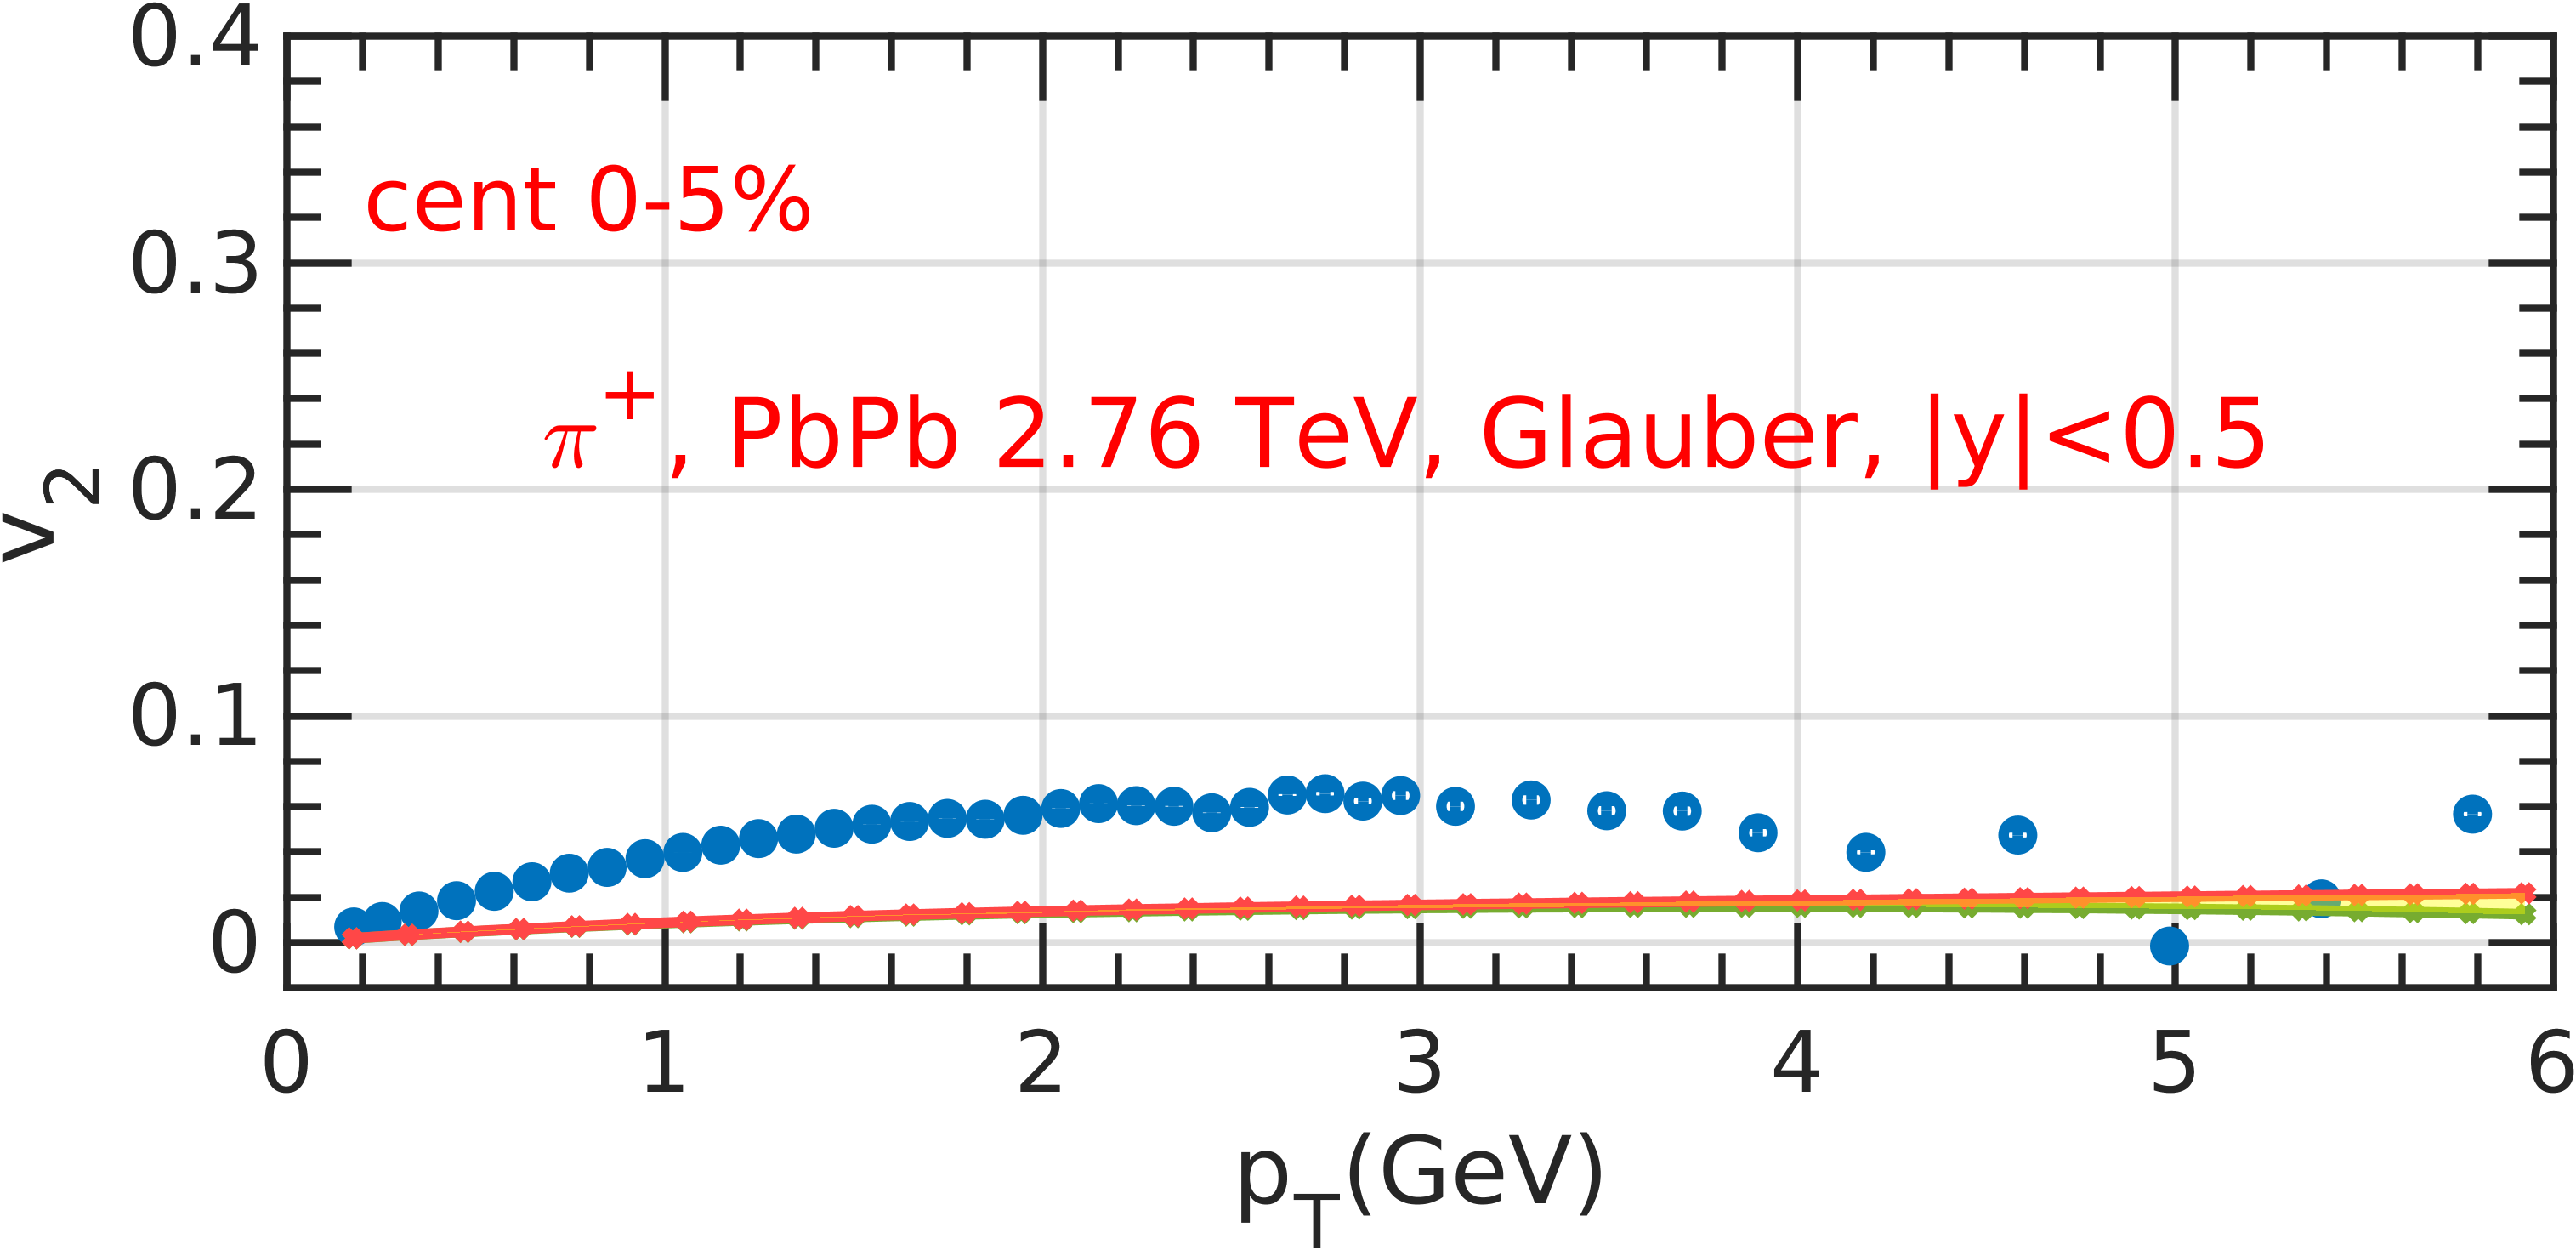
\includegraphics[scale=0.19]{figs/3DGeometric/v2_pT0-5.png}
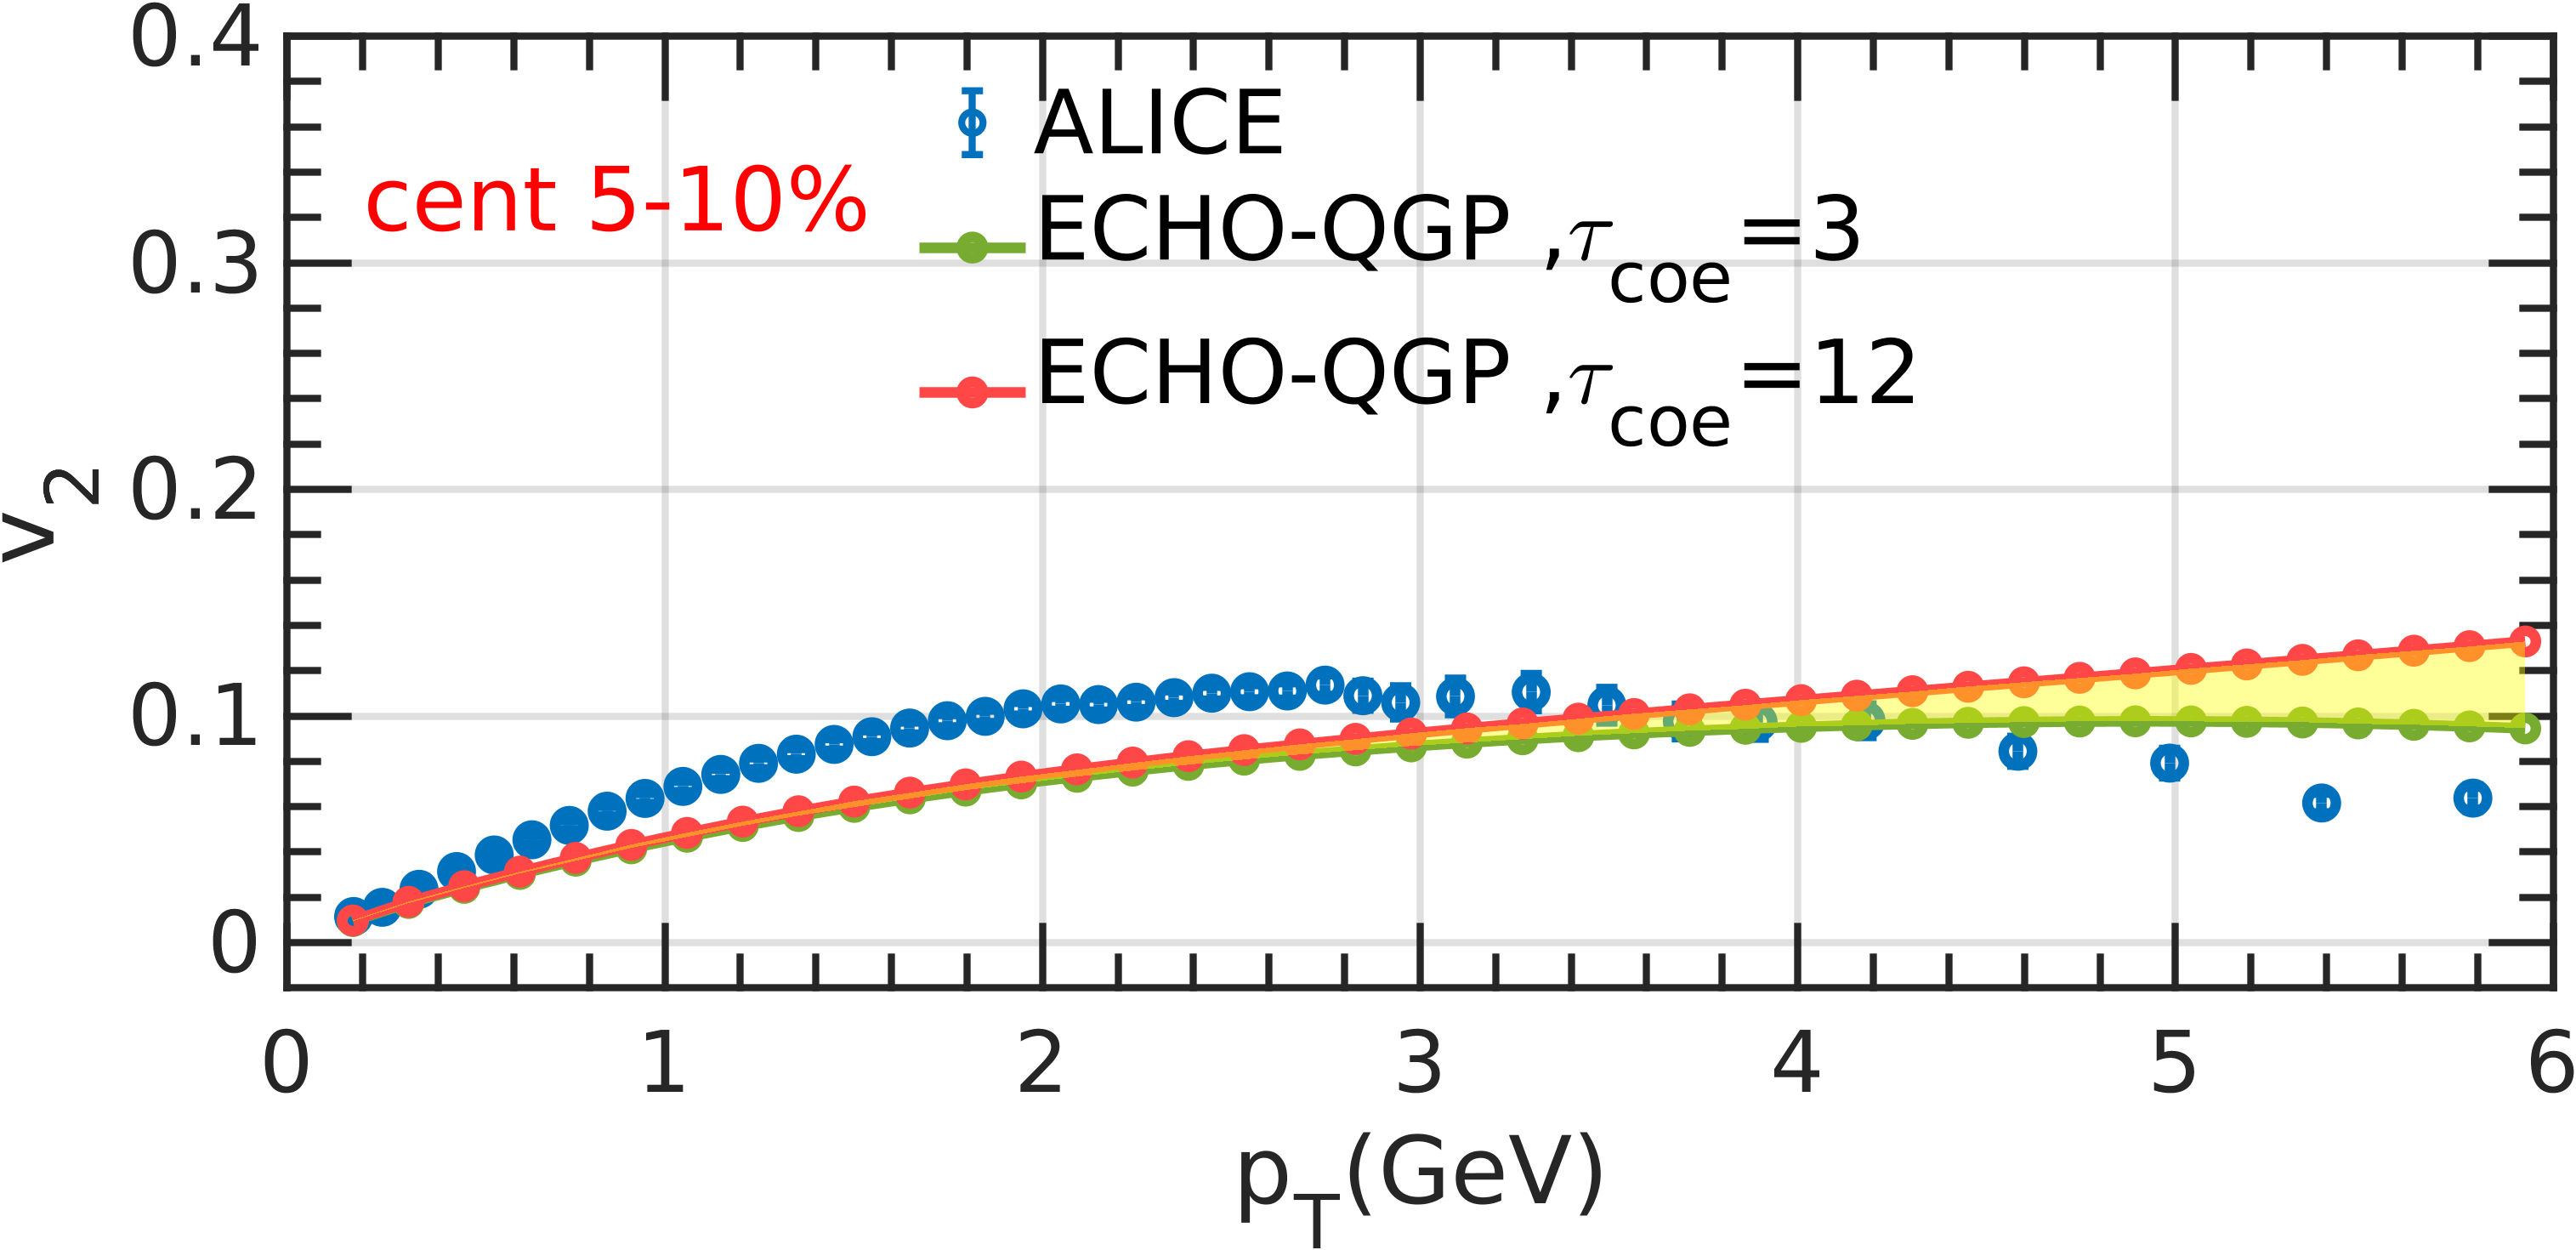
\includegraphics[scale=0.19]{figs/3DGeometric/v2_pT5-10.png}
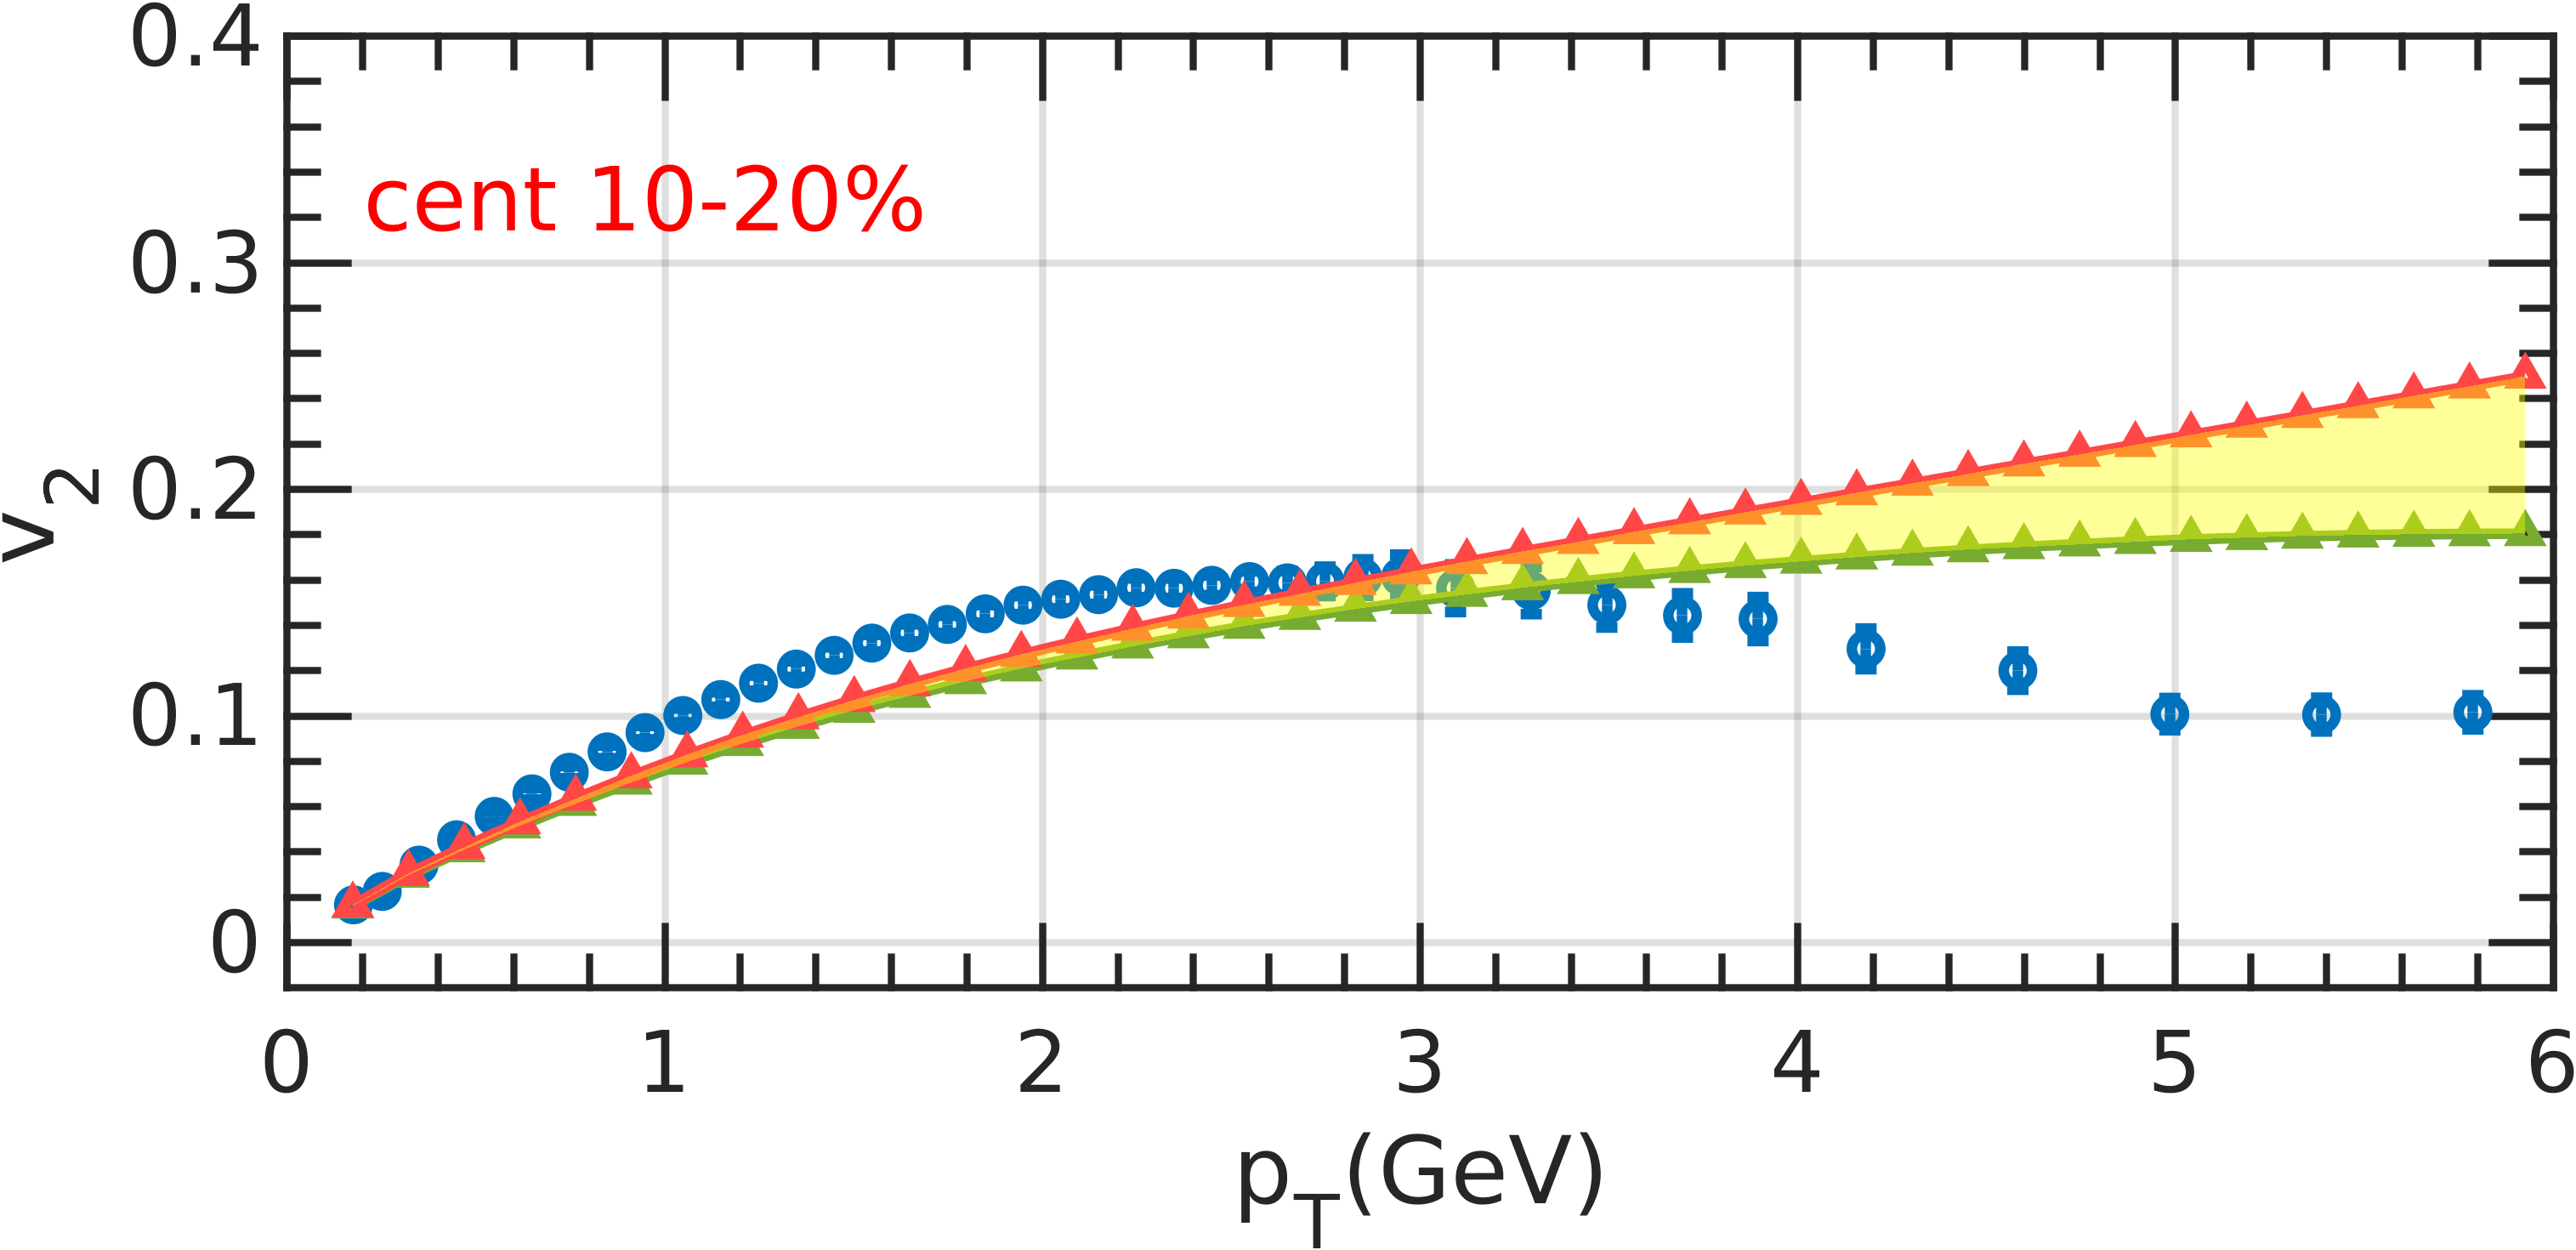
\includegraphics[scale=0.19]{figs/3DGeometric/v2_pT10-20.png}
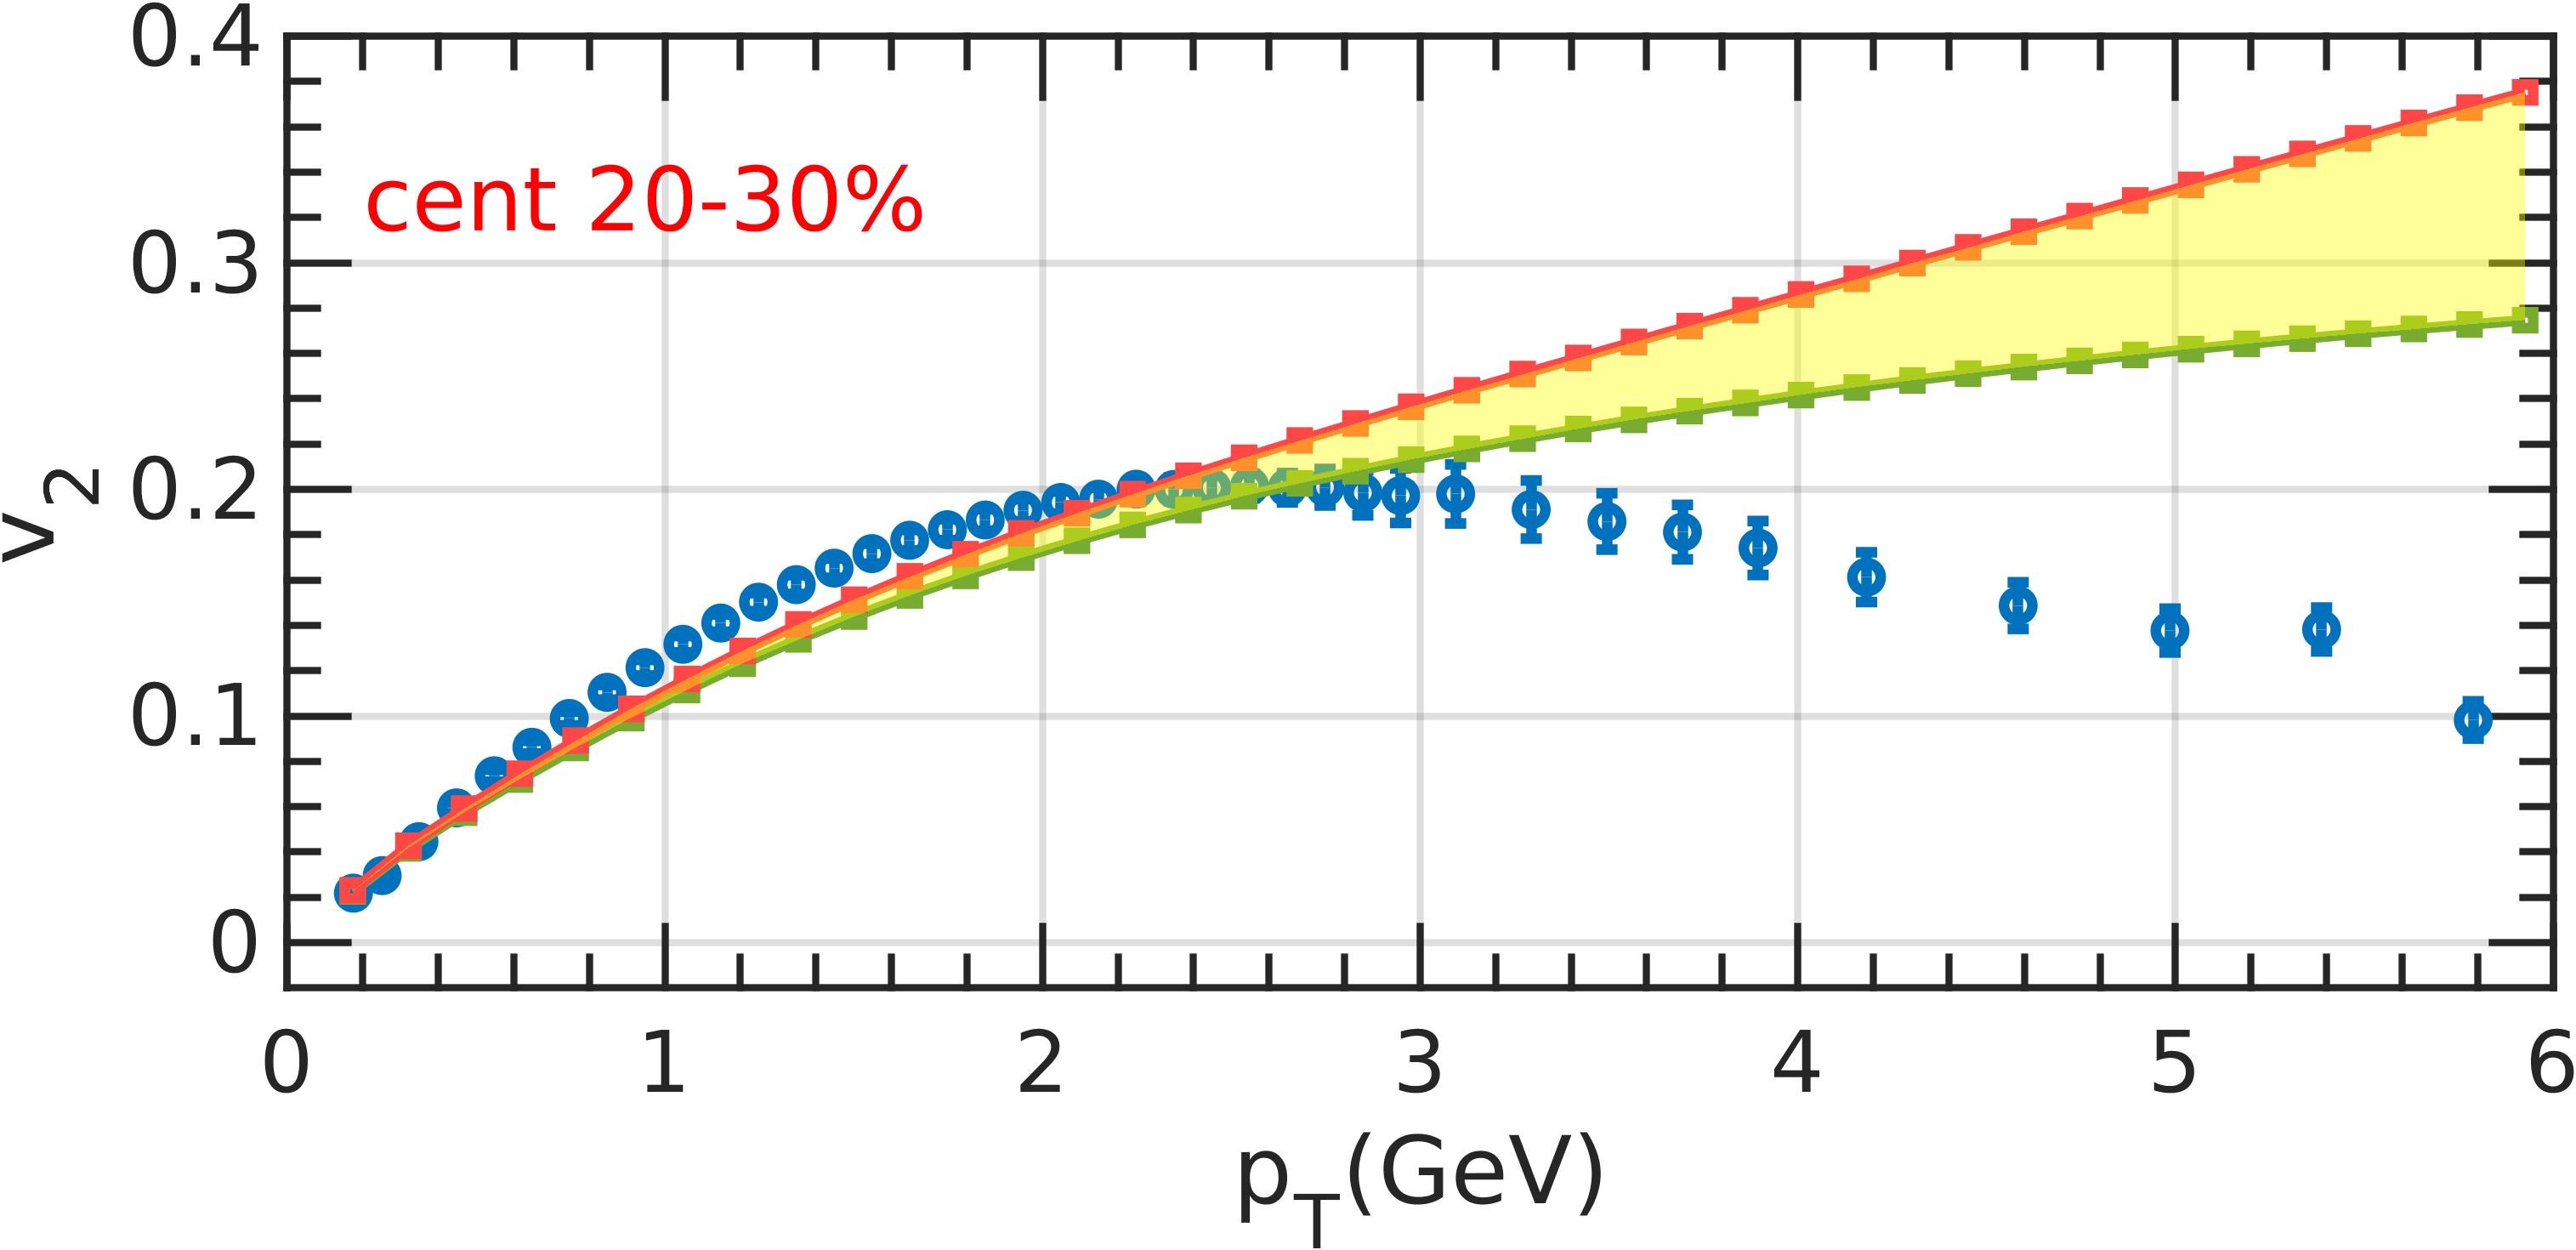
\includegraphics[scale=0.19]{figs/3DGeometric/v2_pT20-30.png}
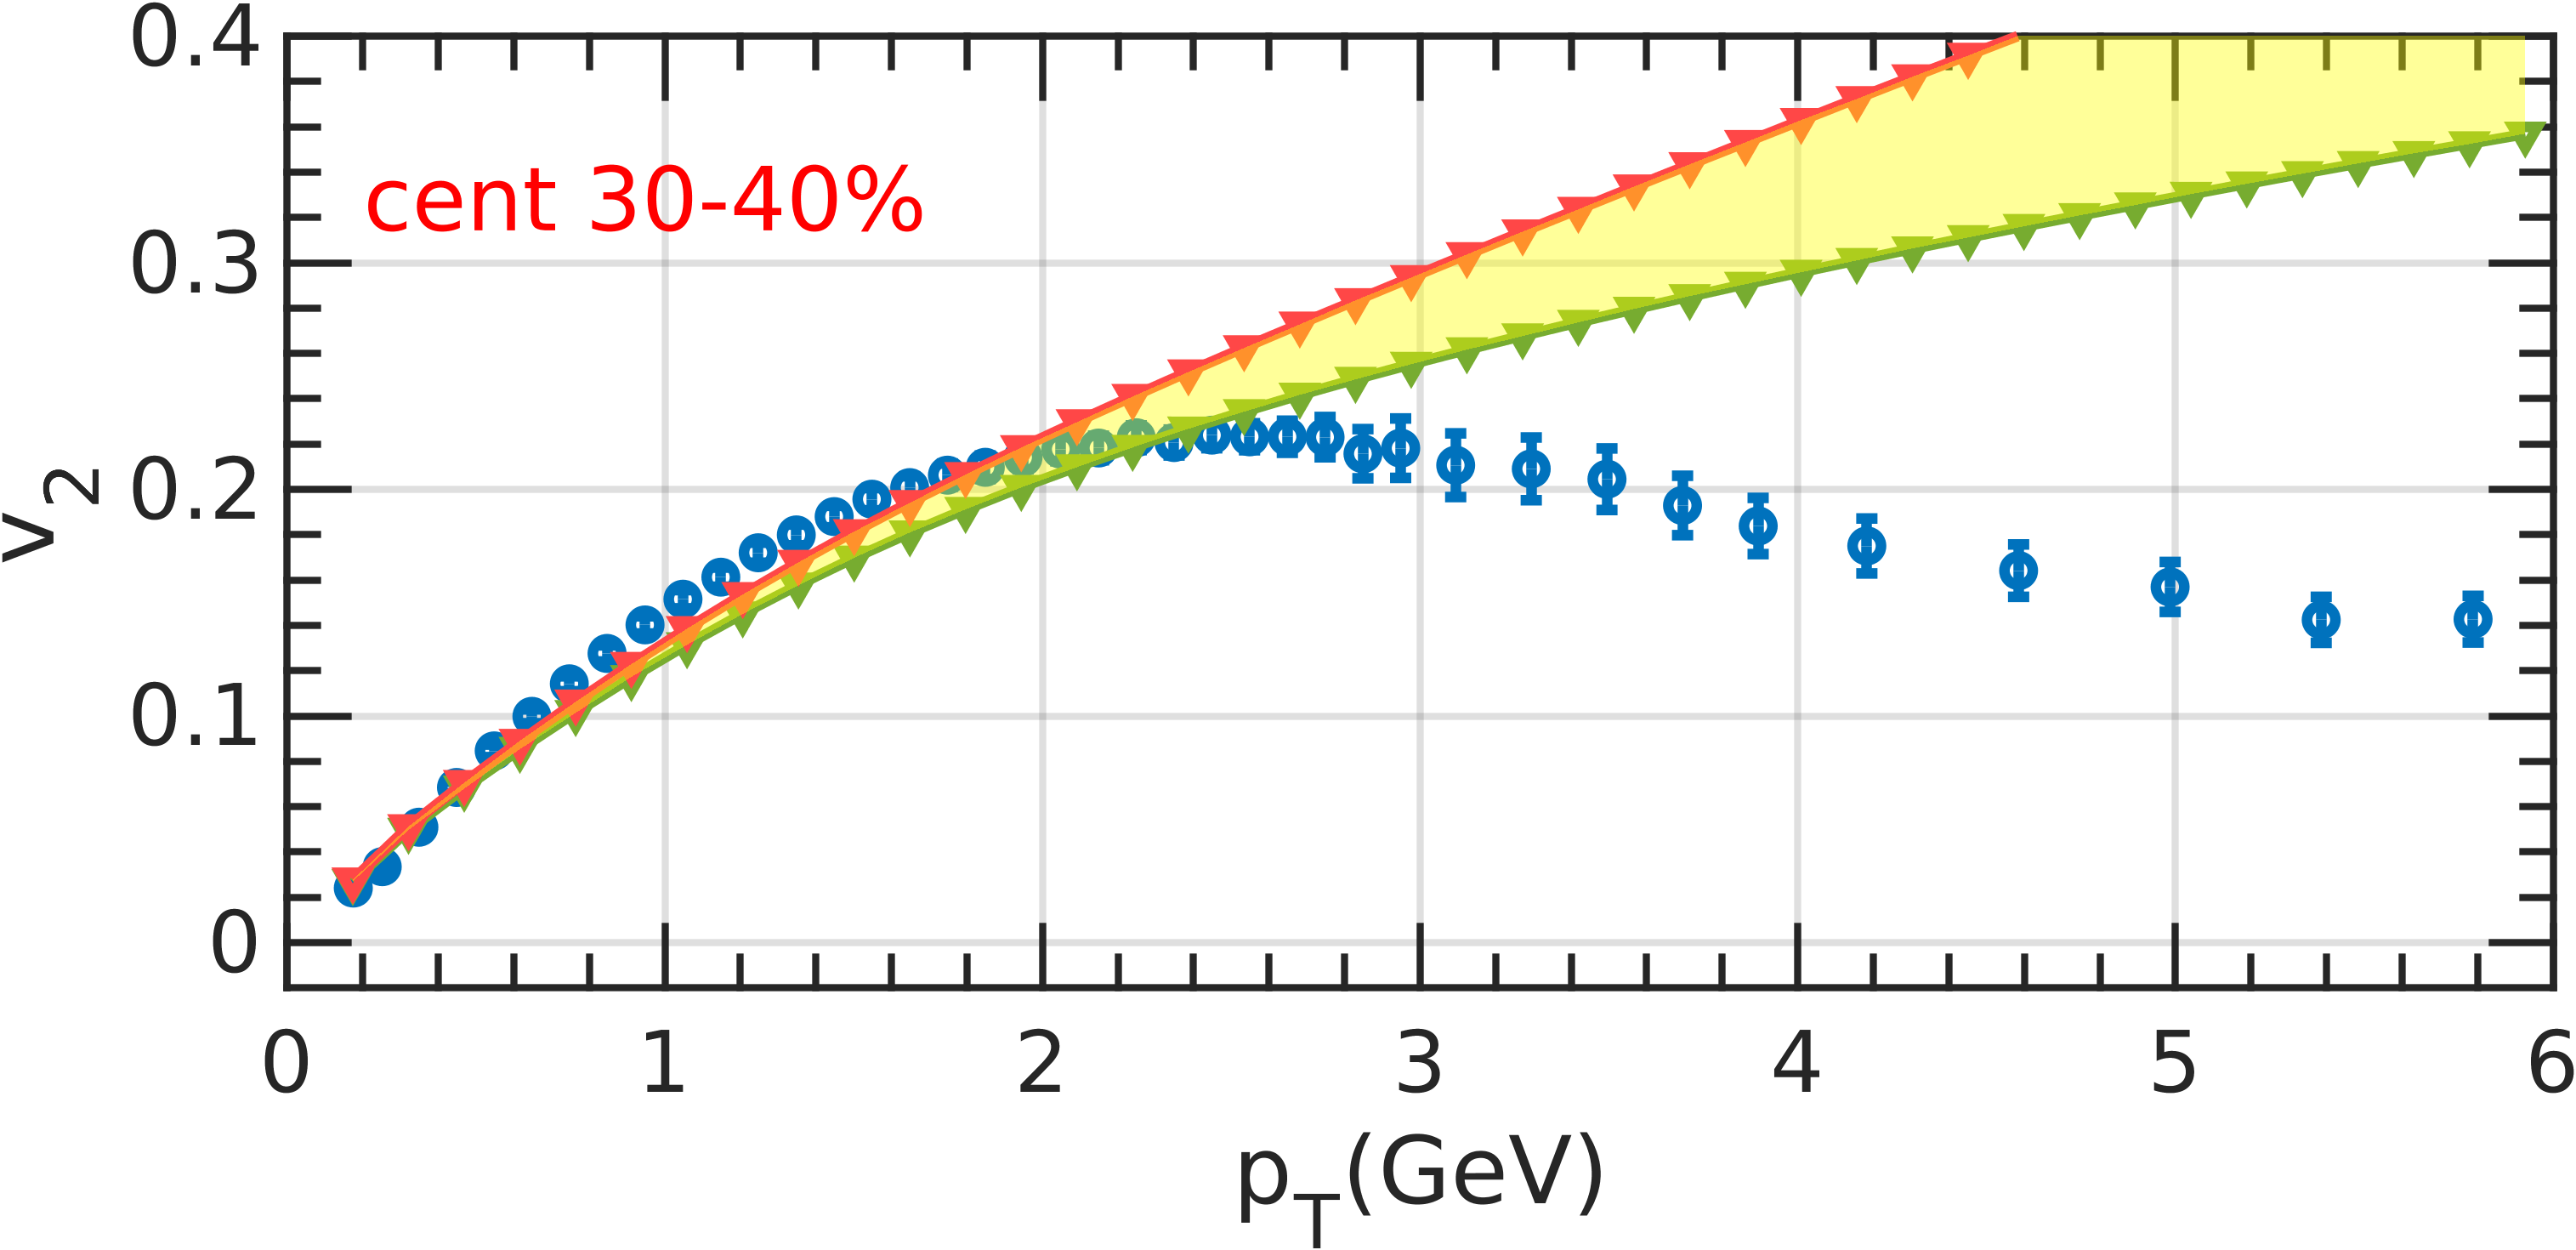
\includegraphics[scale=0.19]{figs/3DGeometric/v2_pT30-40.png}
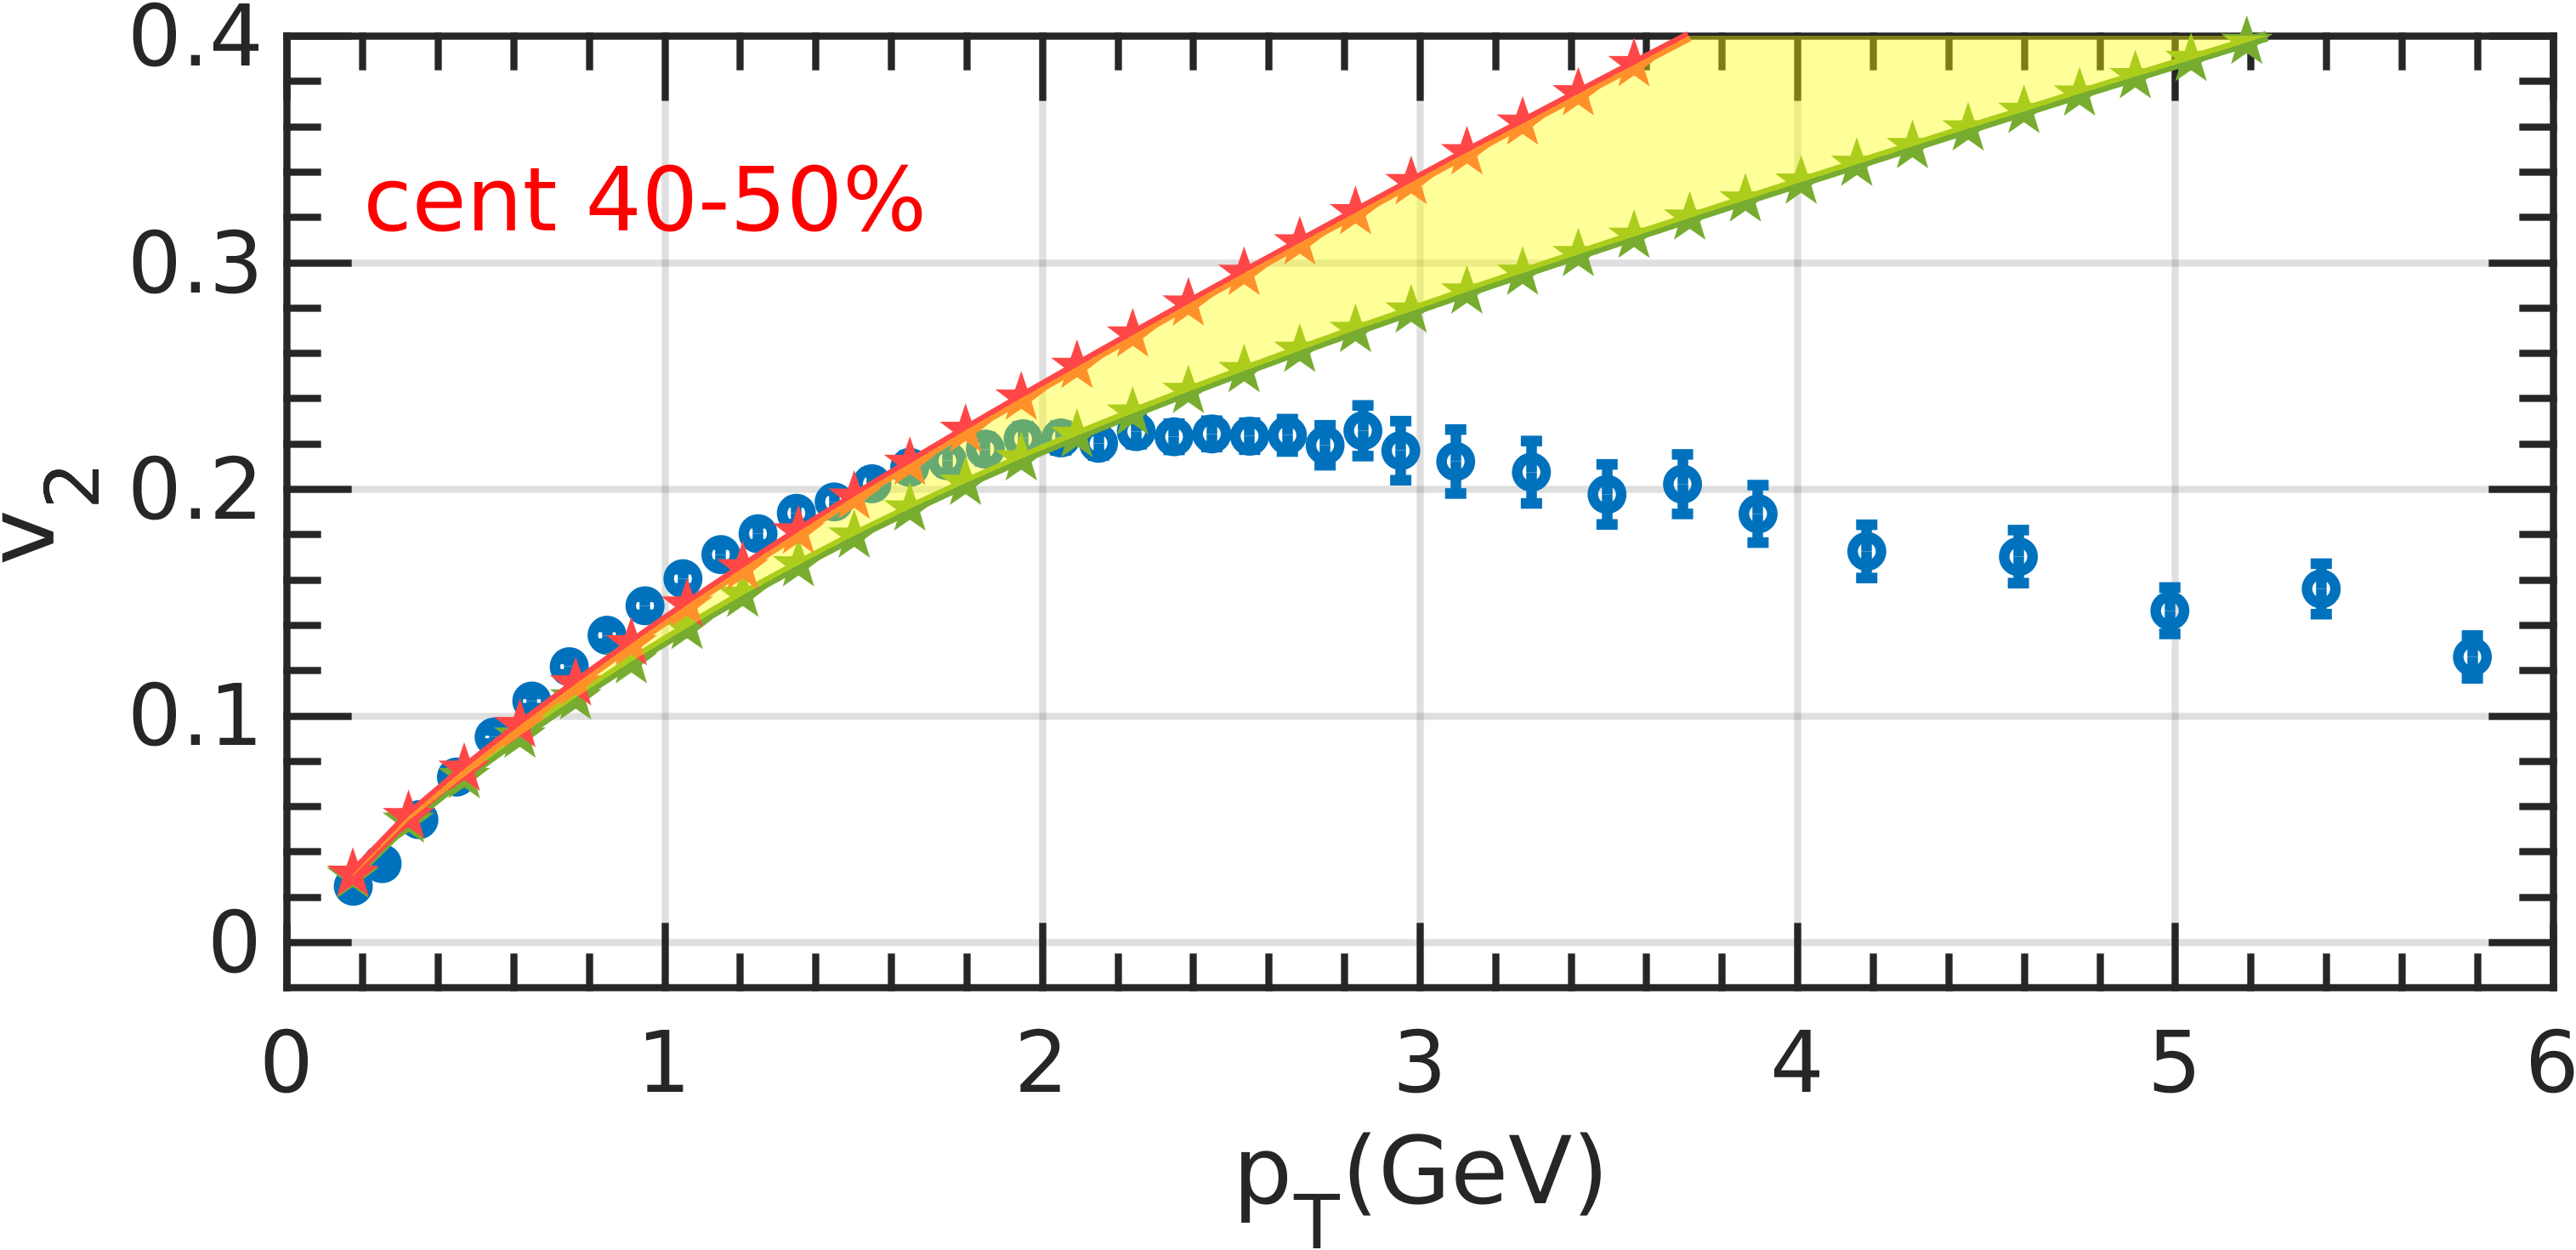
\includegraphics[scale=0.19]{figs/3DGeometric/v2_pT40-50.png}
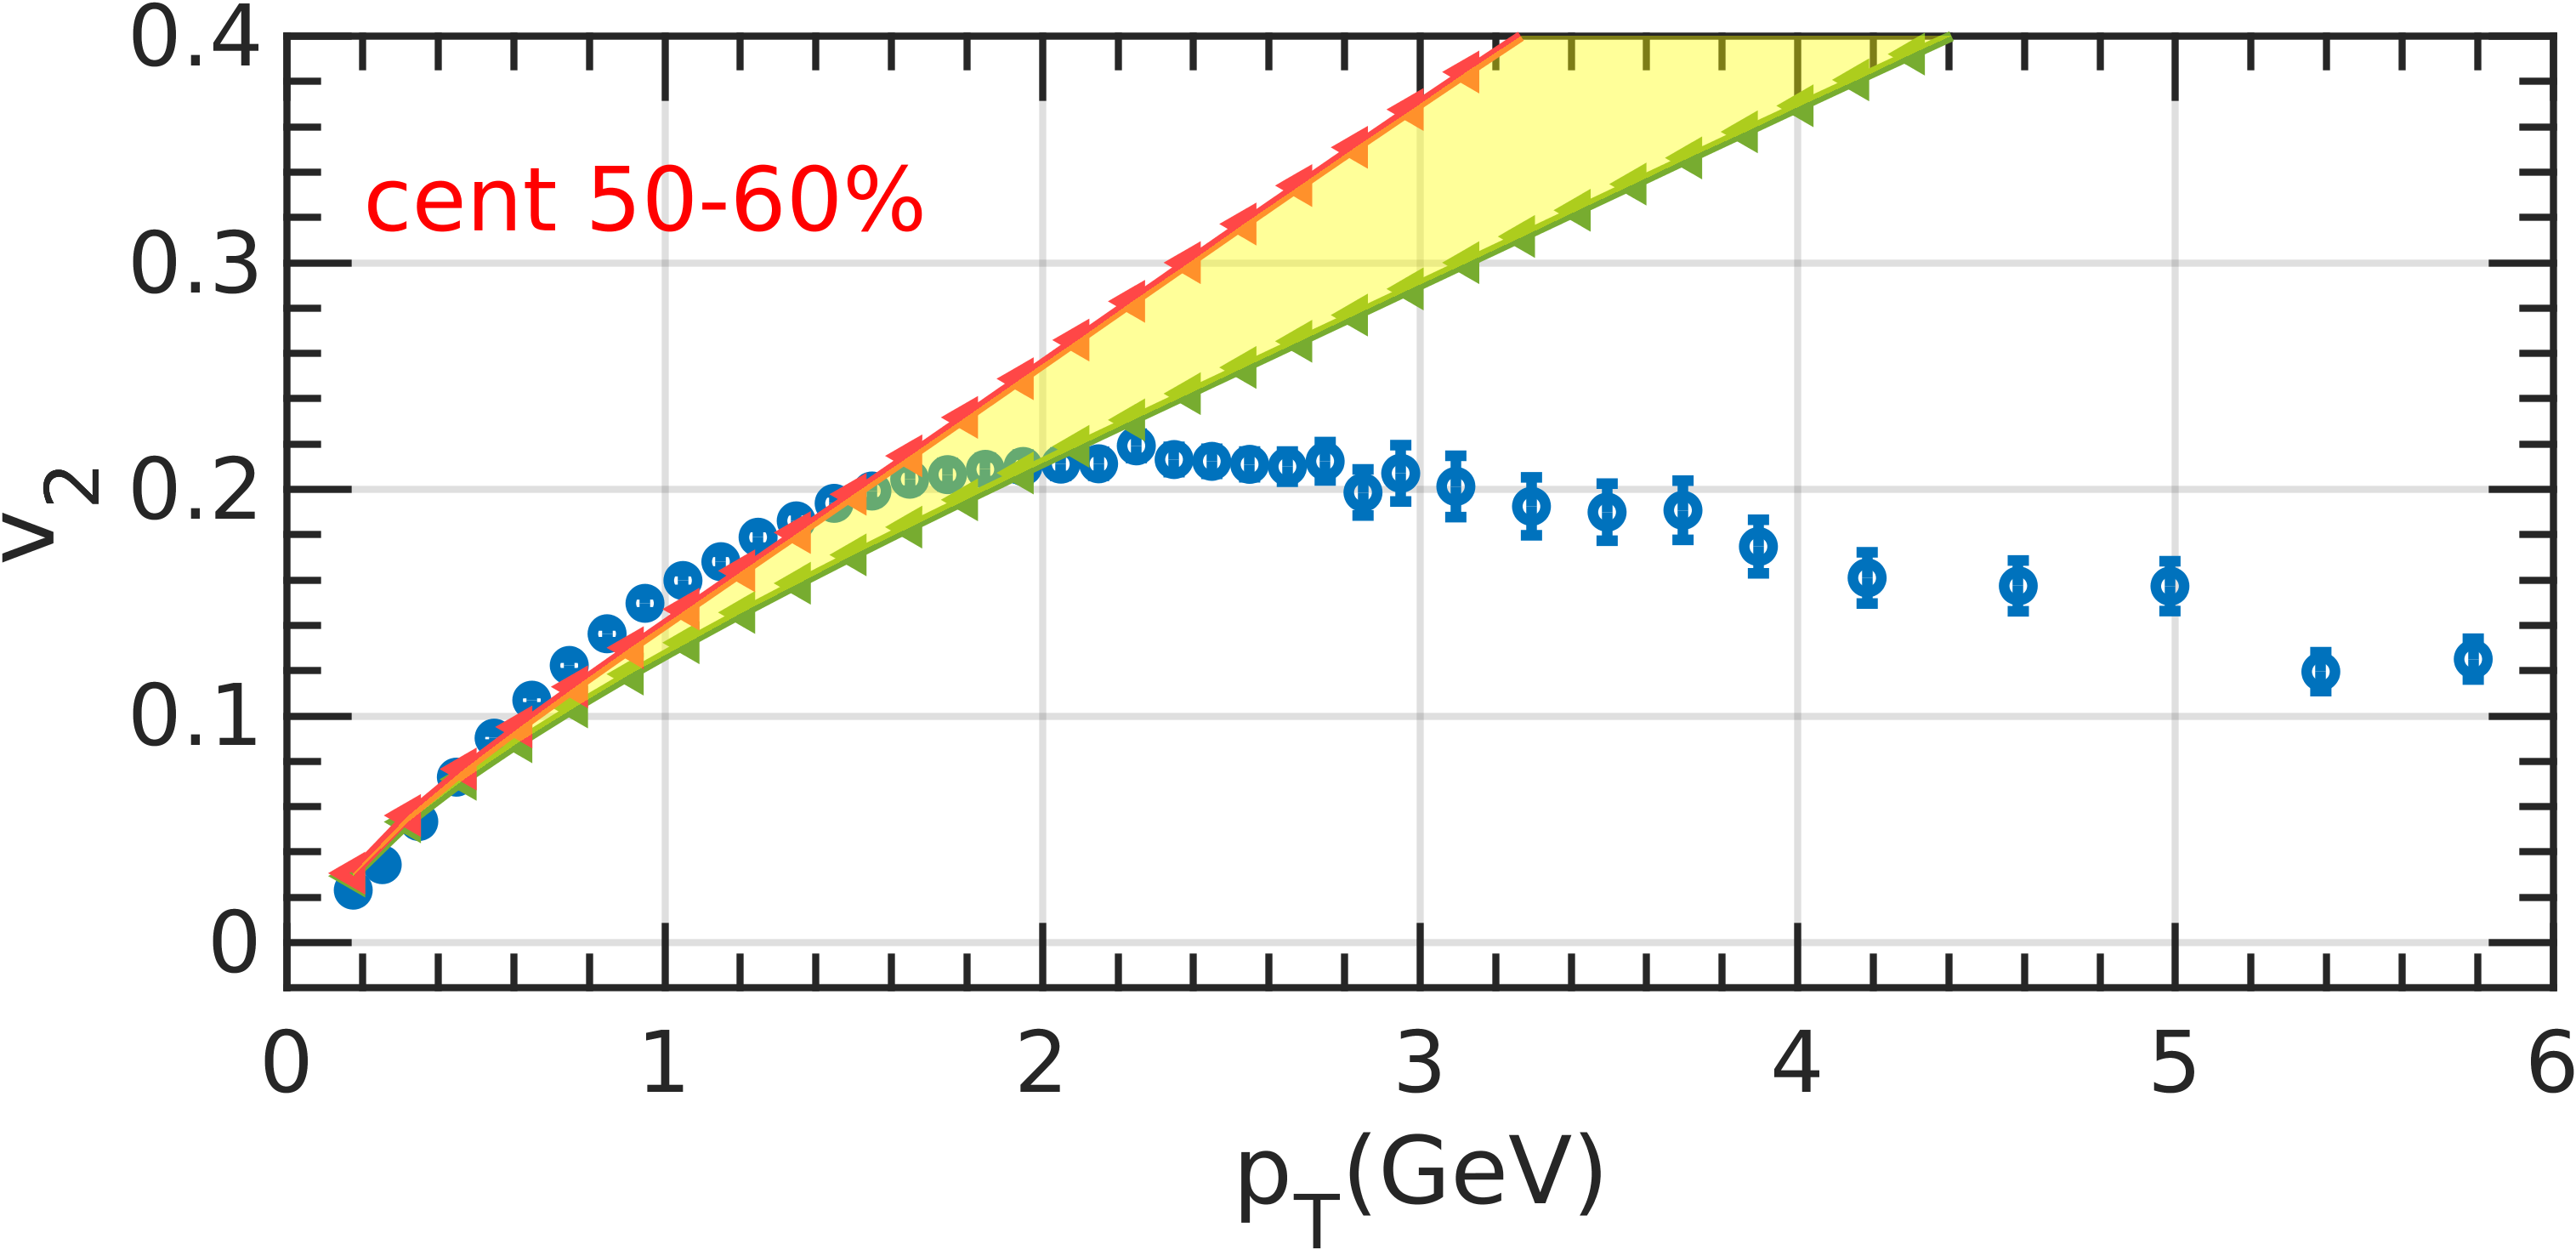
\includegraphics[scale=0.19]{figs/3DGeometric/v2_pT50-60.png}
%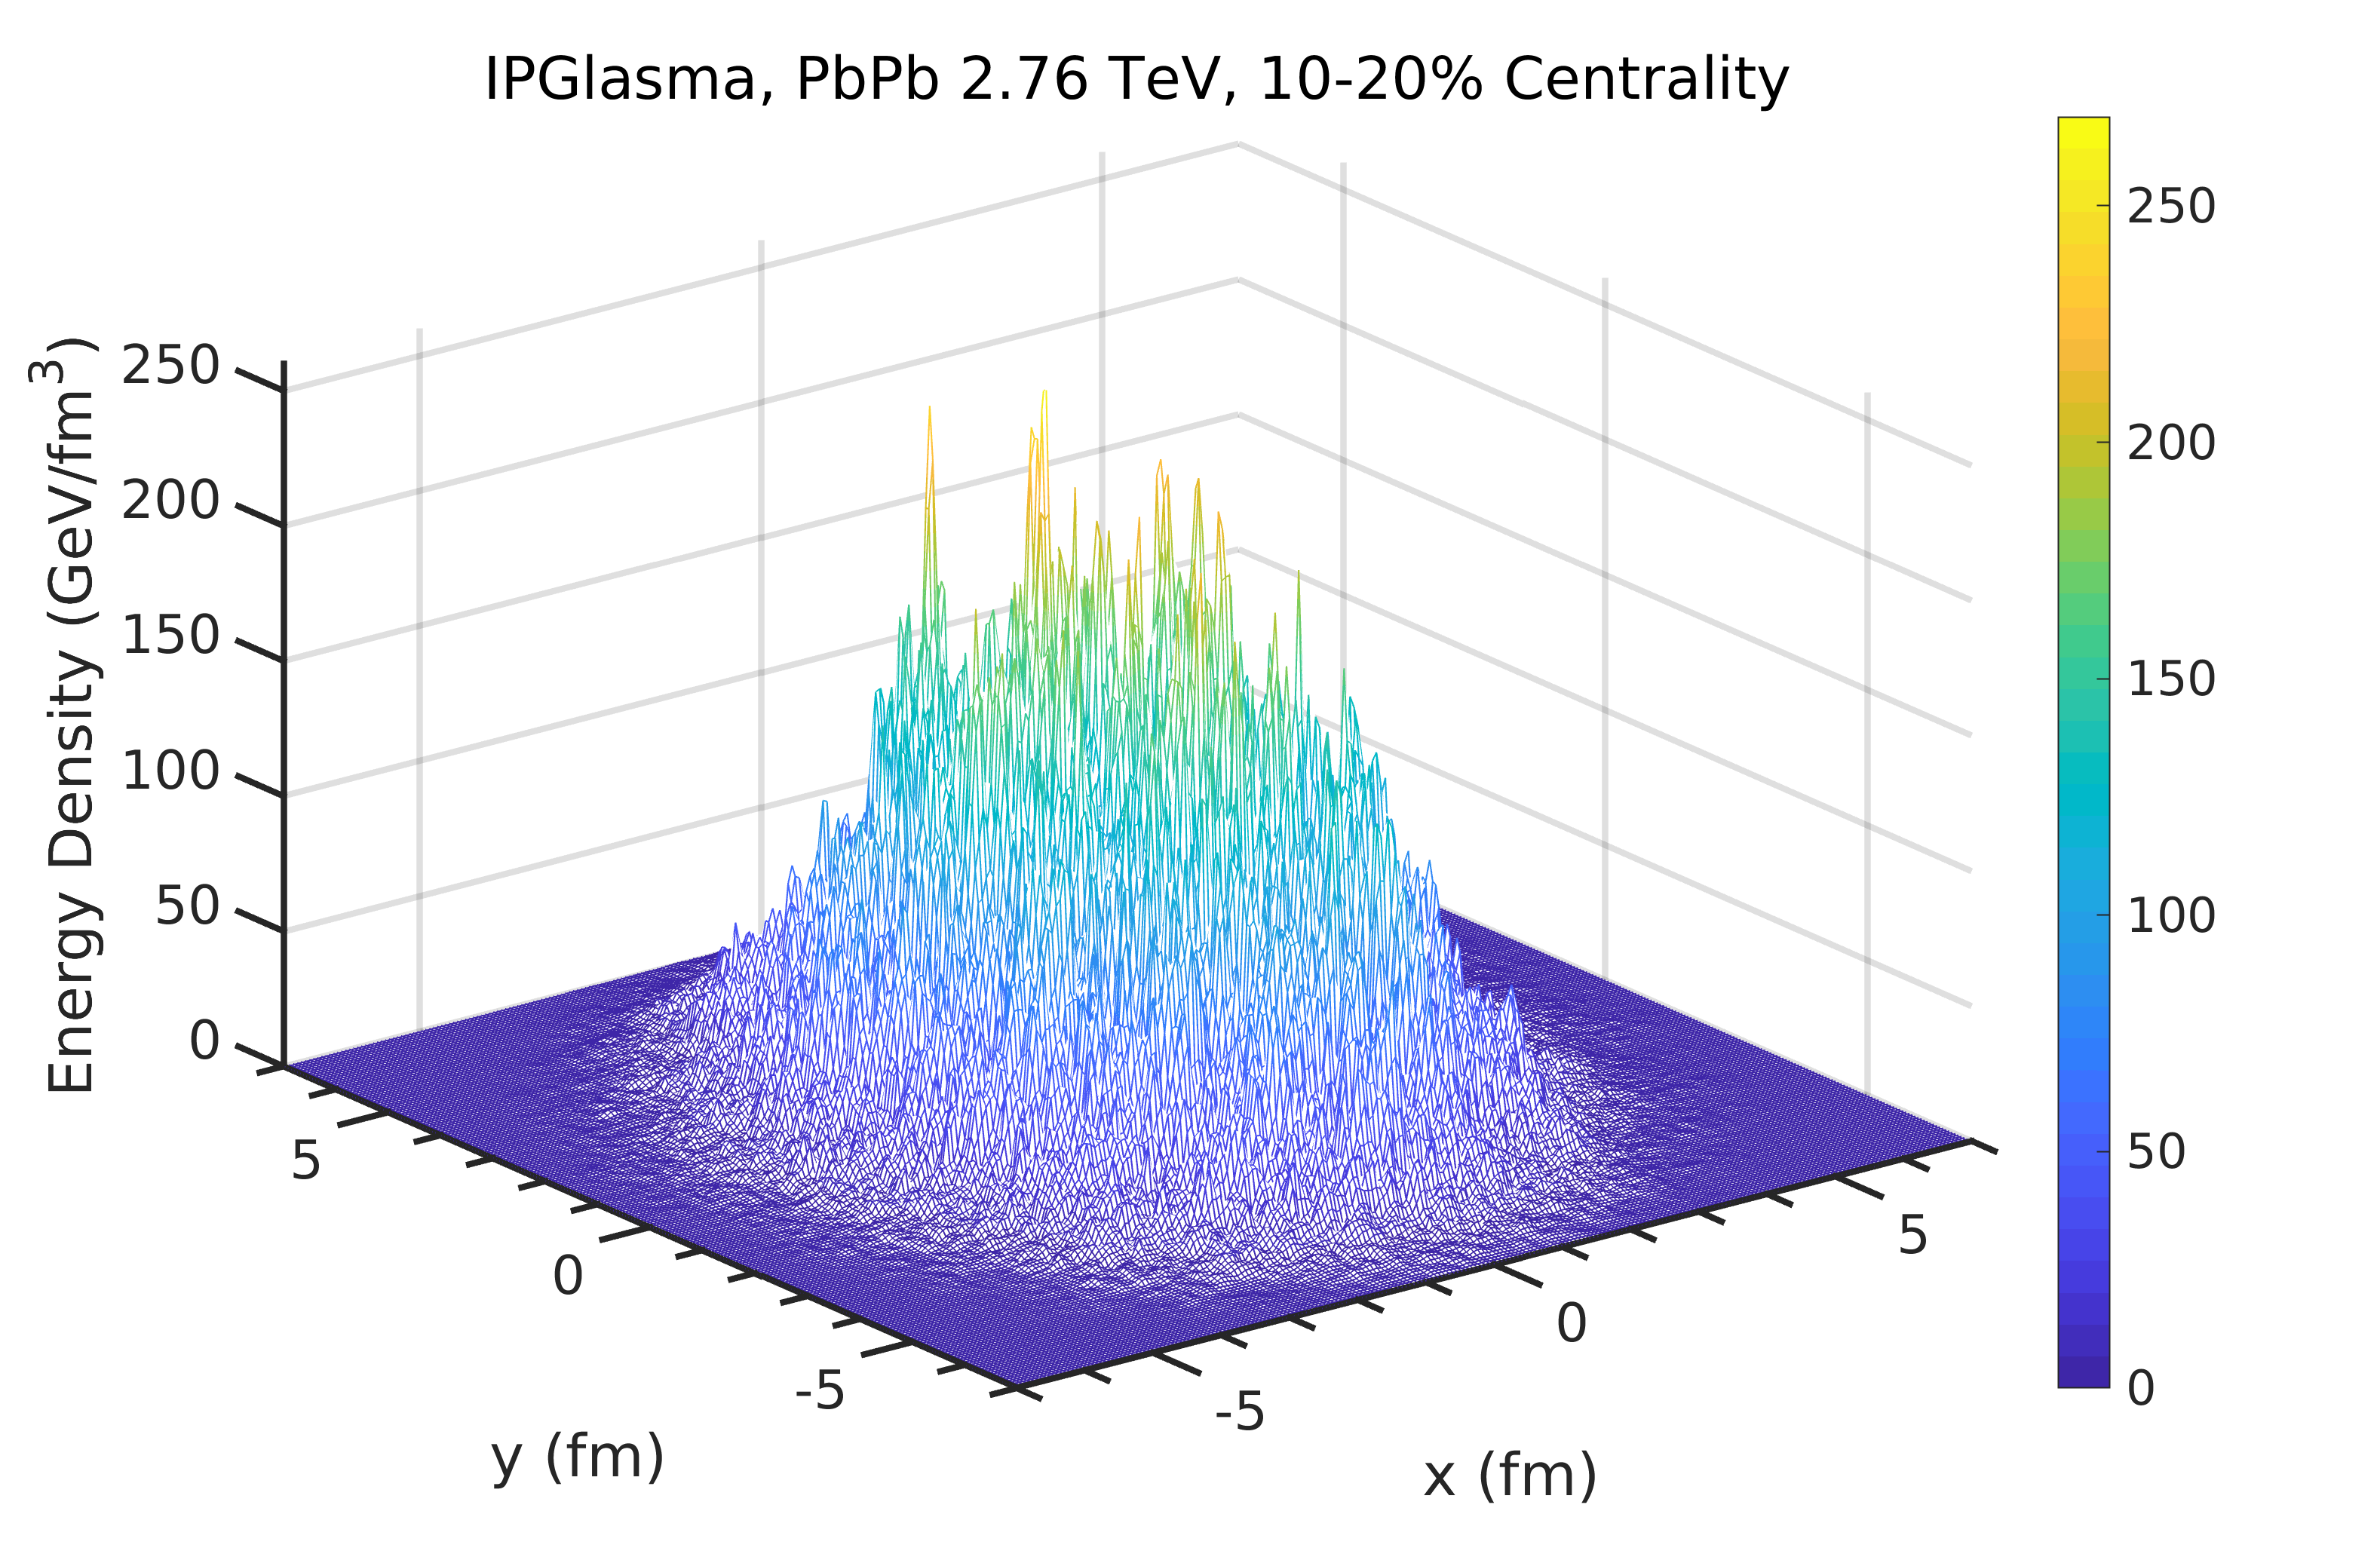
\includegraphics[scale=0.22]{figs/IPGlasma.png}
\end{figure}

Shaded area represents increase in flow due to the use of the larger relaxation time.


\end{frame}

%------------------------------------------------



\begin{frame}

\frametitle{Effect of non-hydro mode in IPGlasma elliptic flow}

\begin{figure}
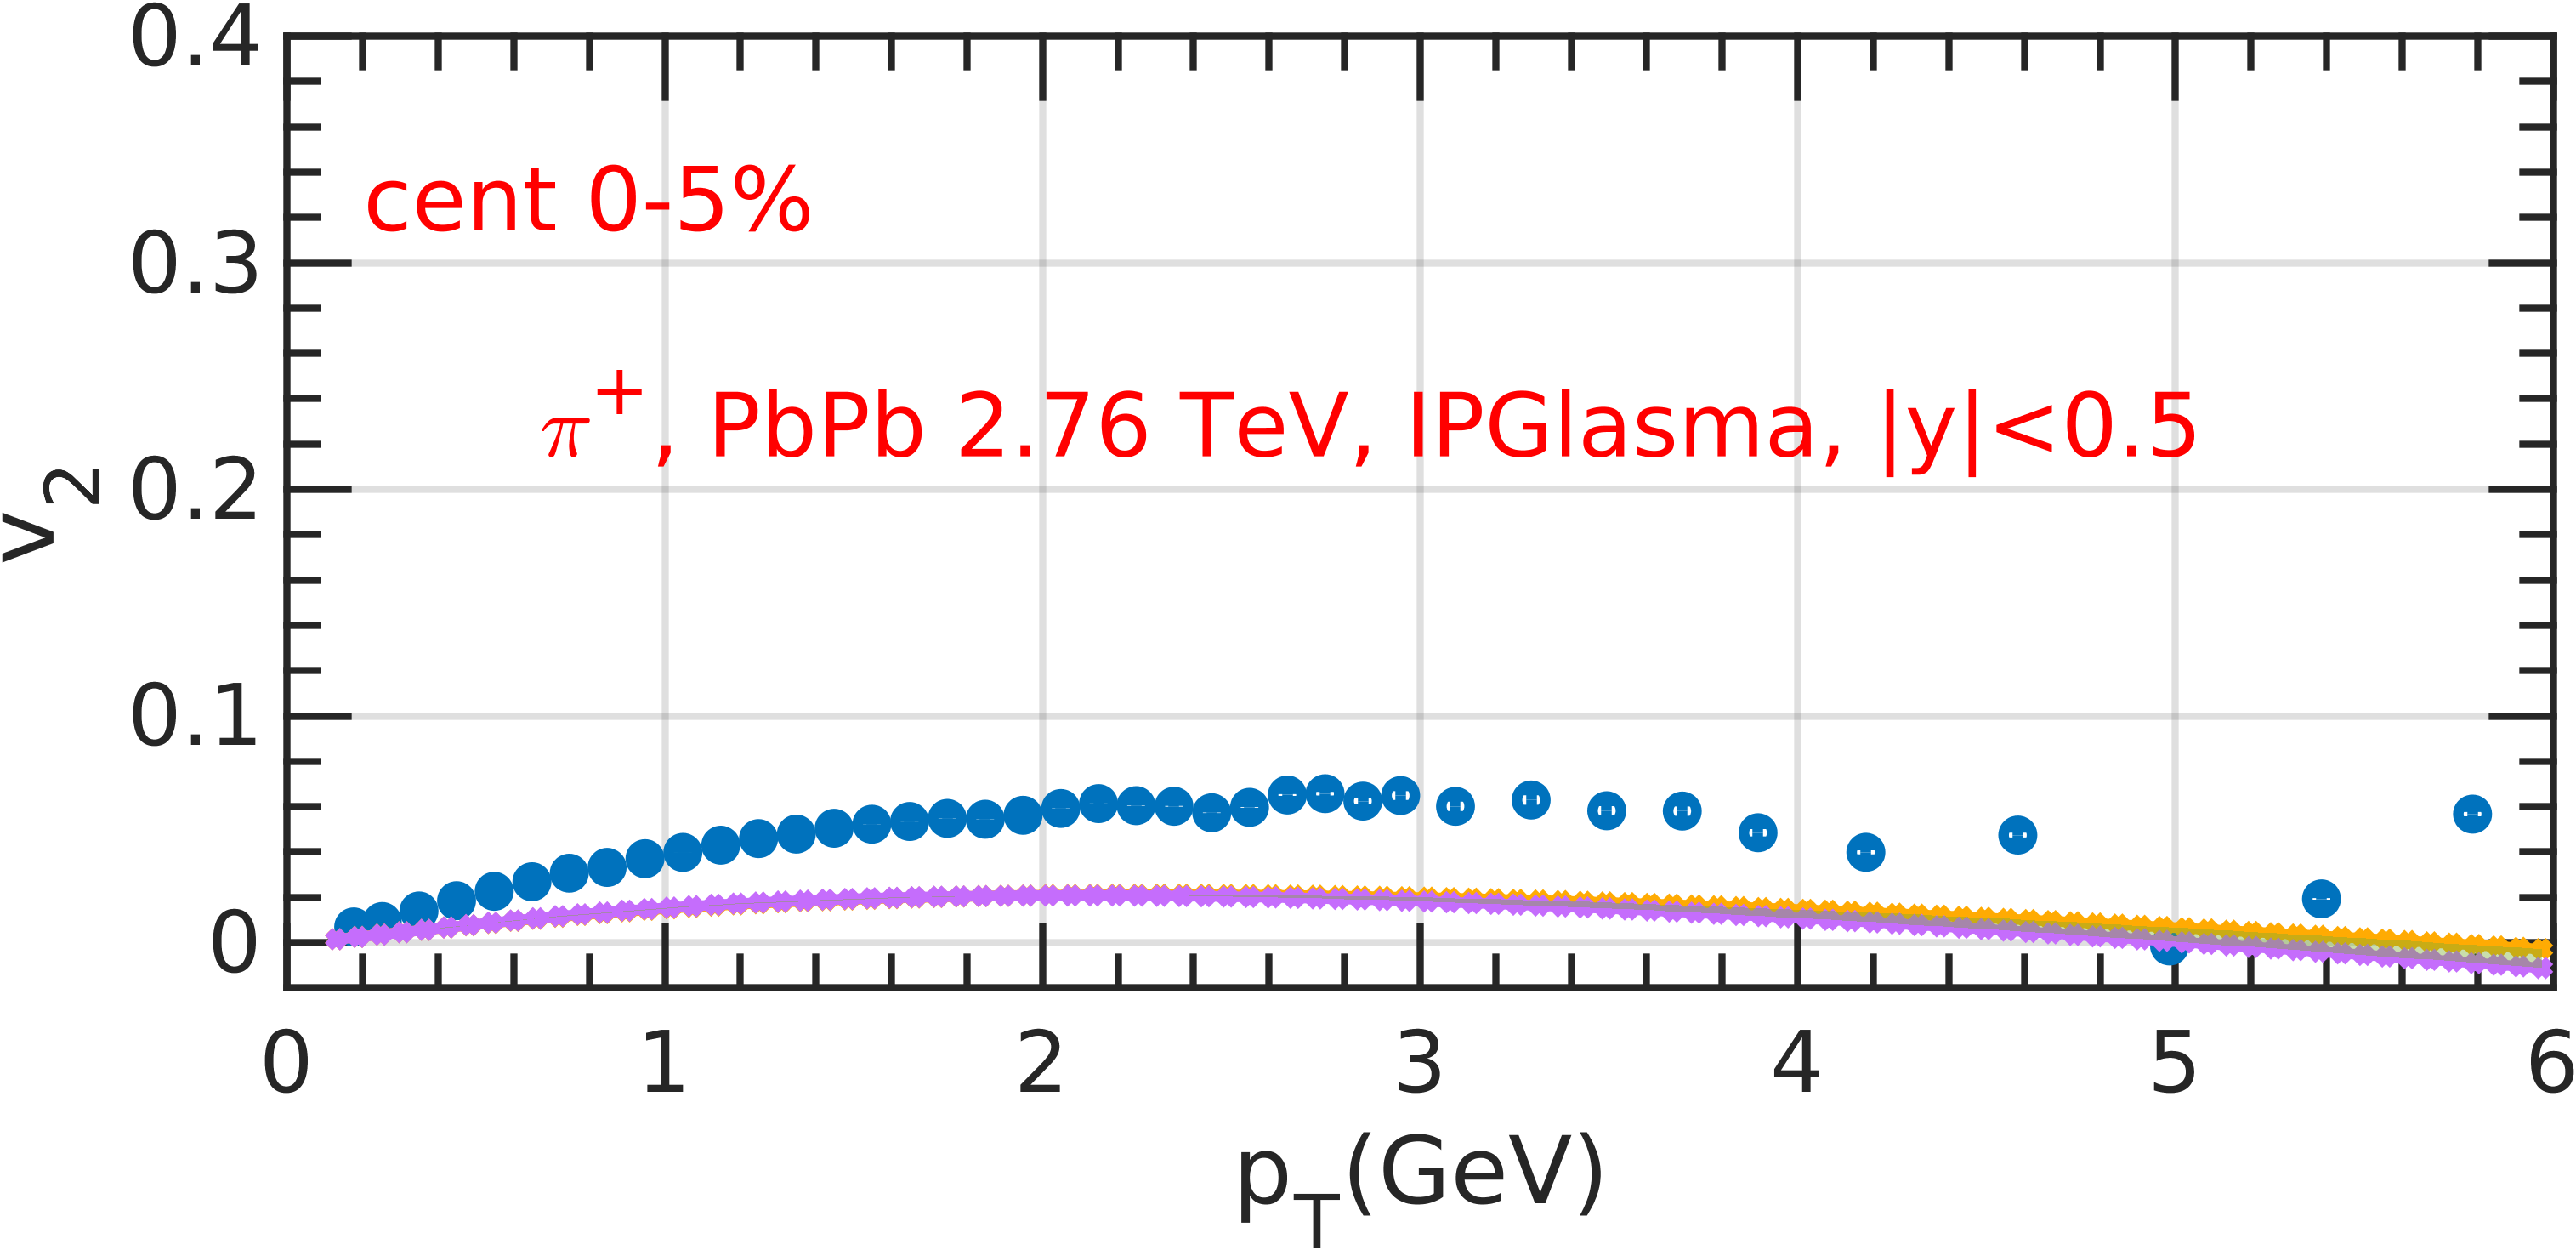
\includegraphics[scale=0.19]{figs/IPGlasma/v2_pT0-5.png}
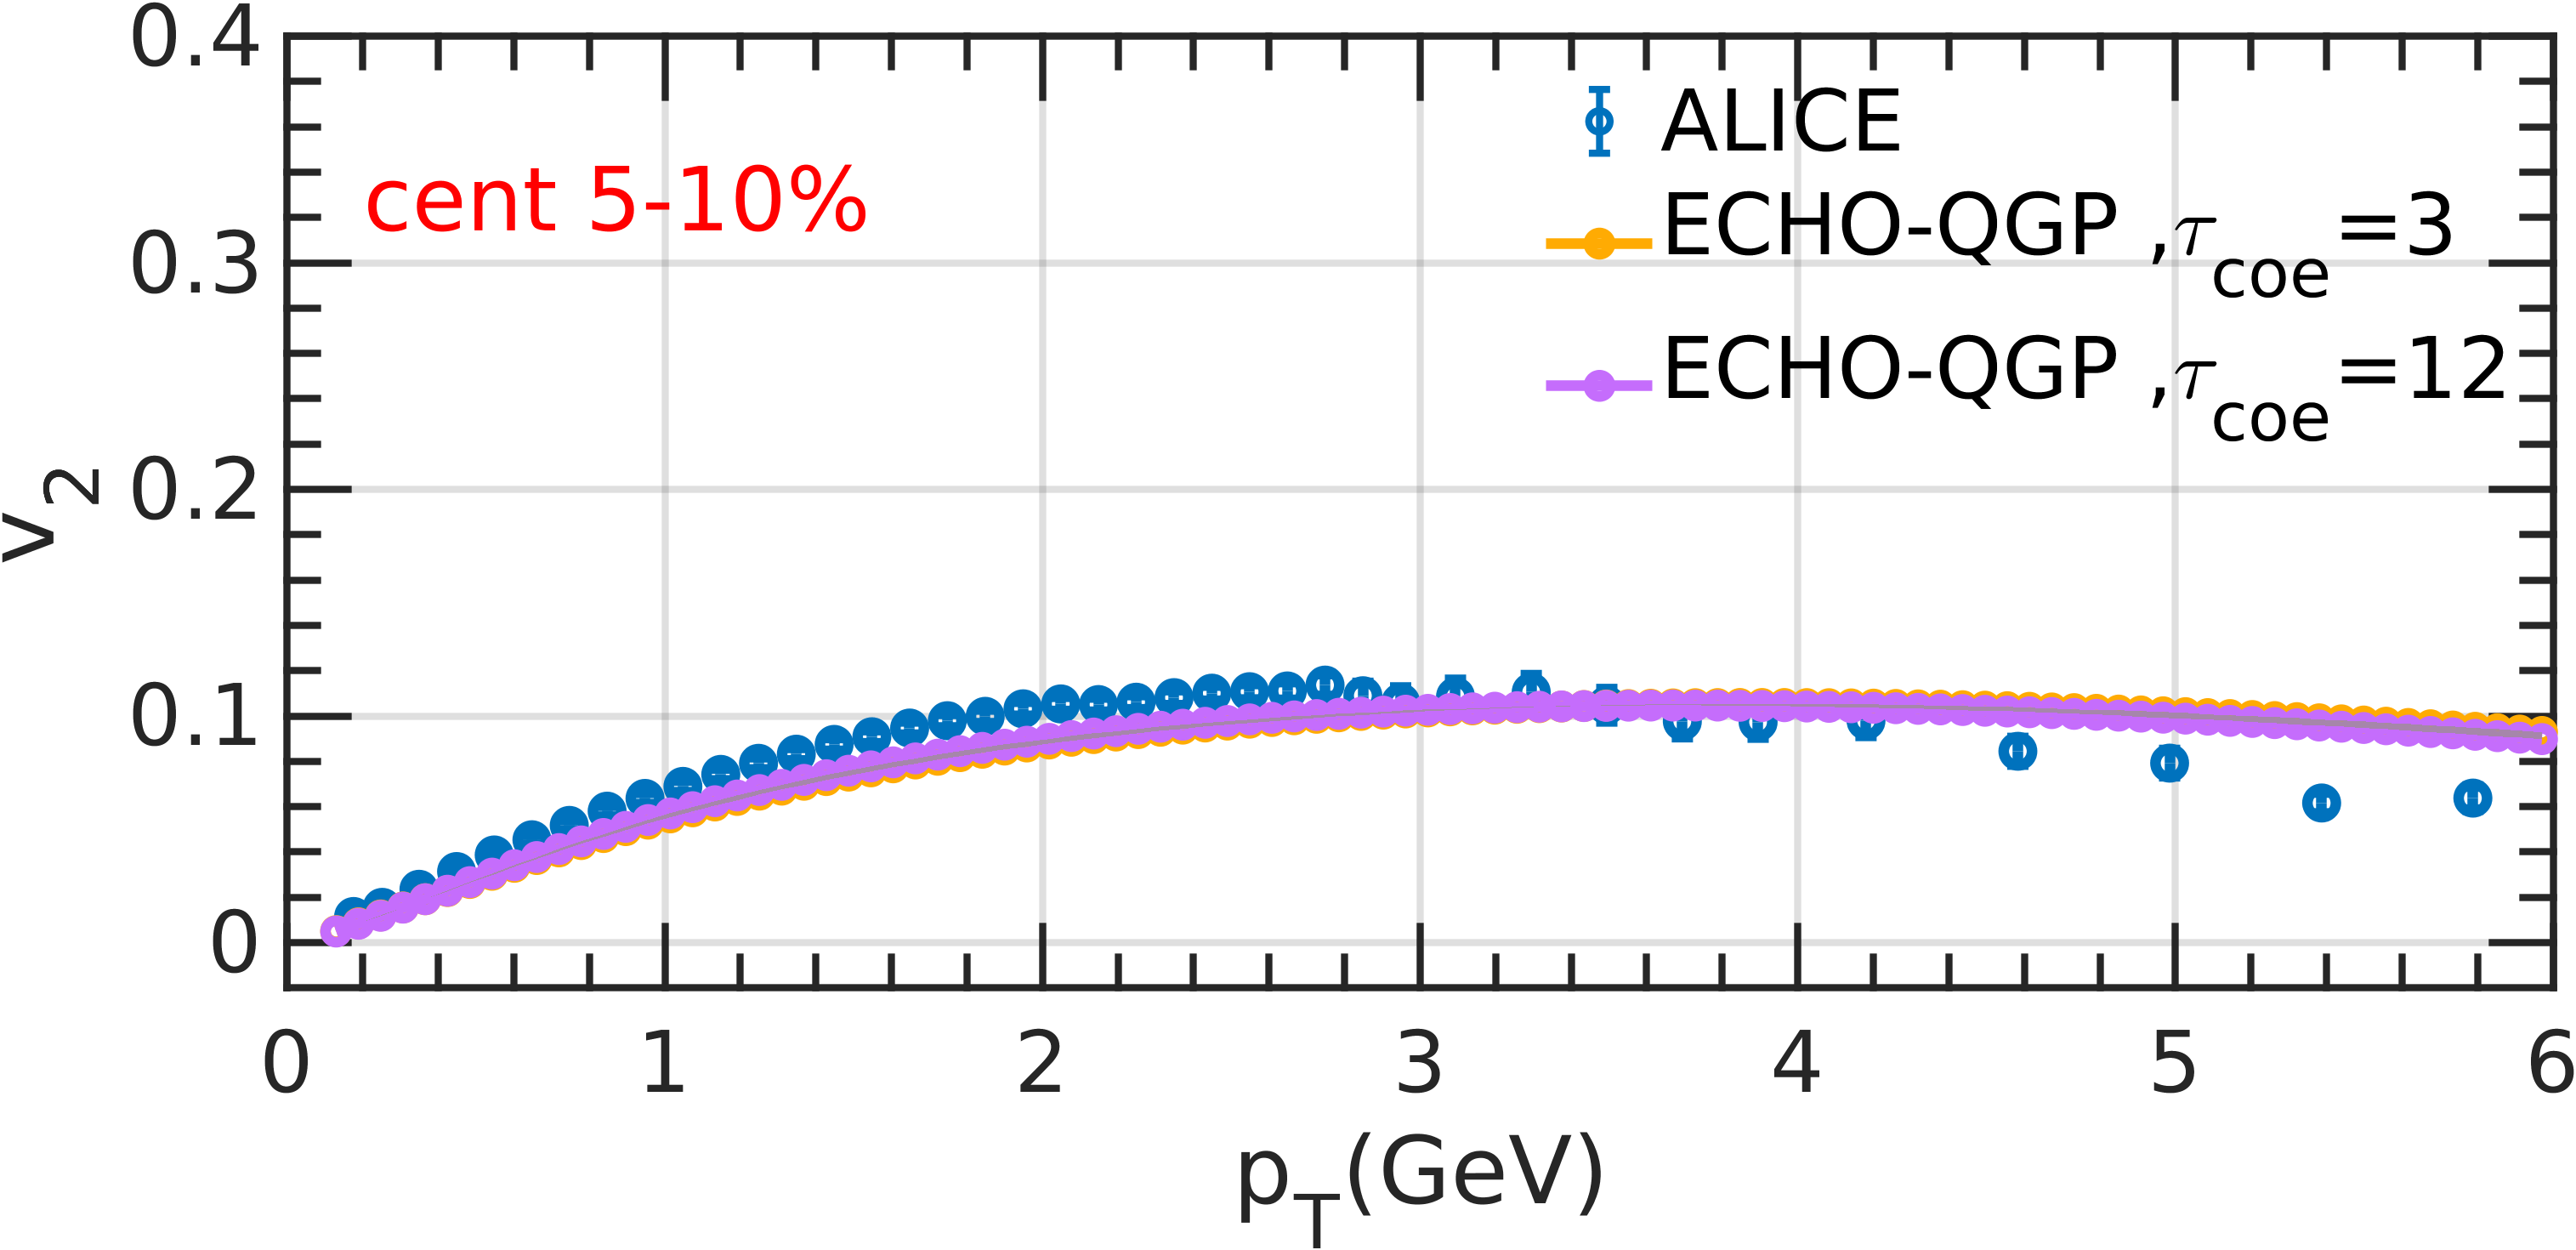
\includegraphics[scale=0.19]{figs/IPGlasma/v2_pT5-10.png}
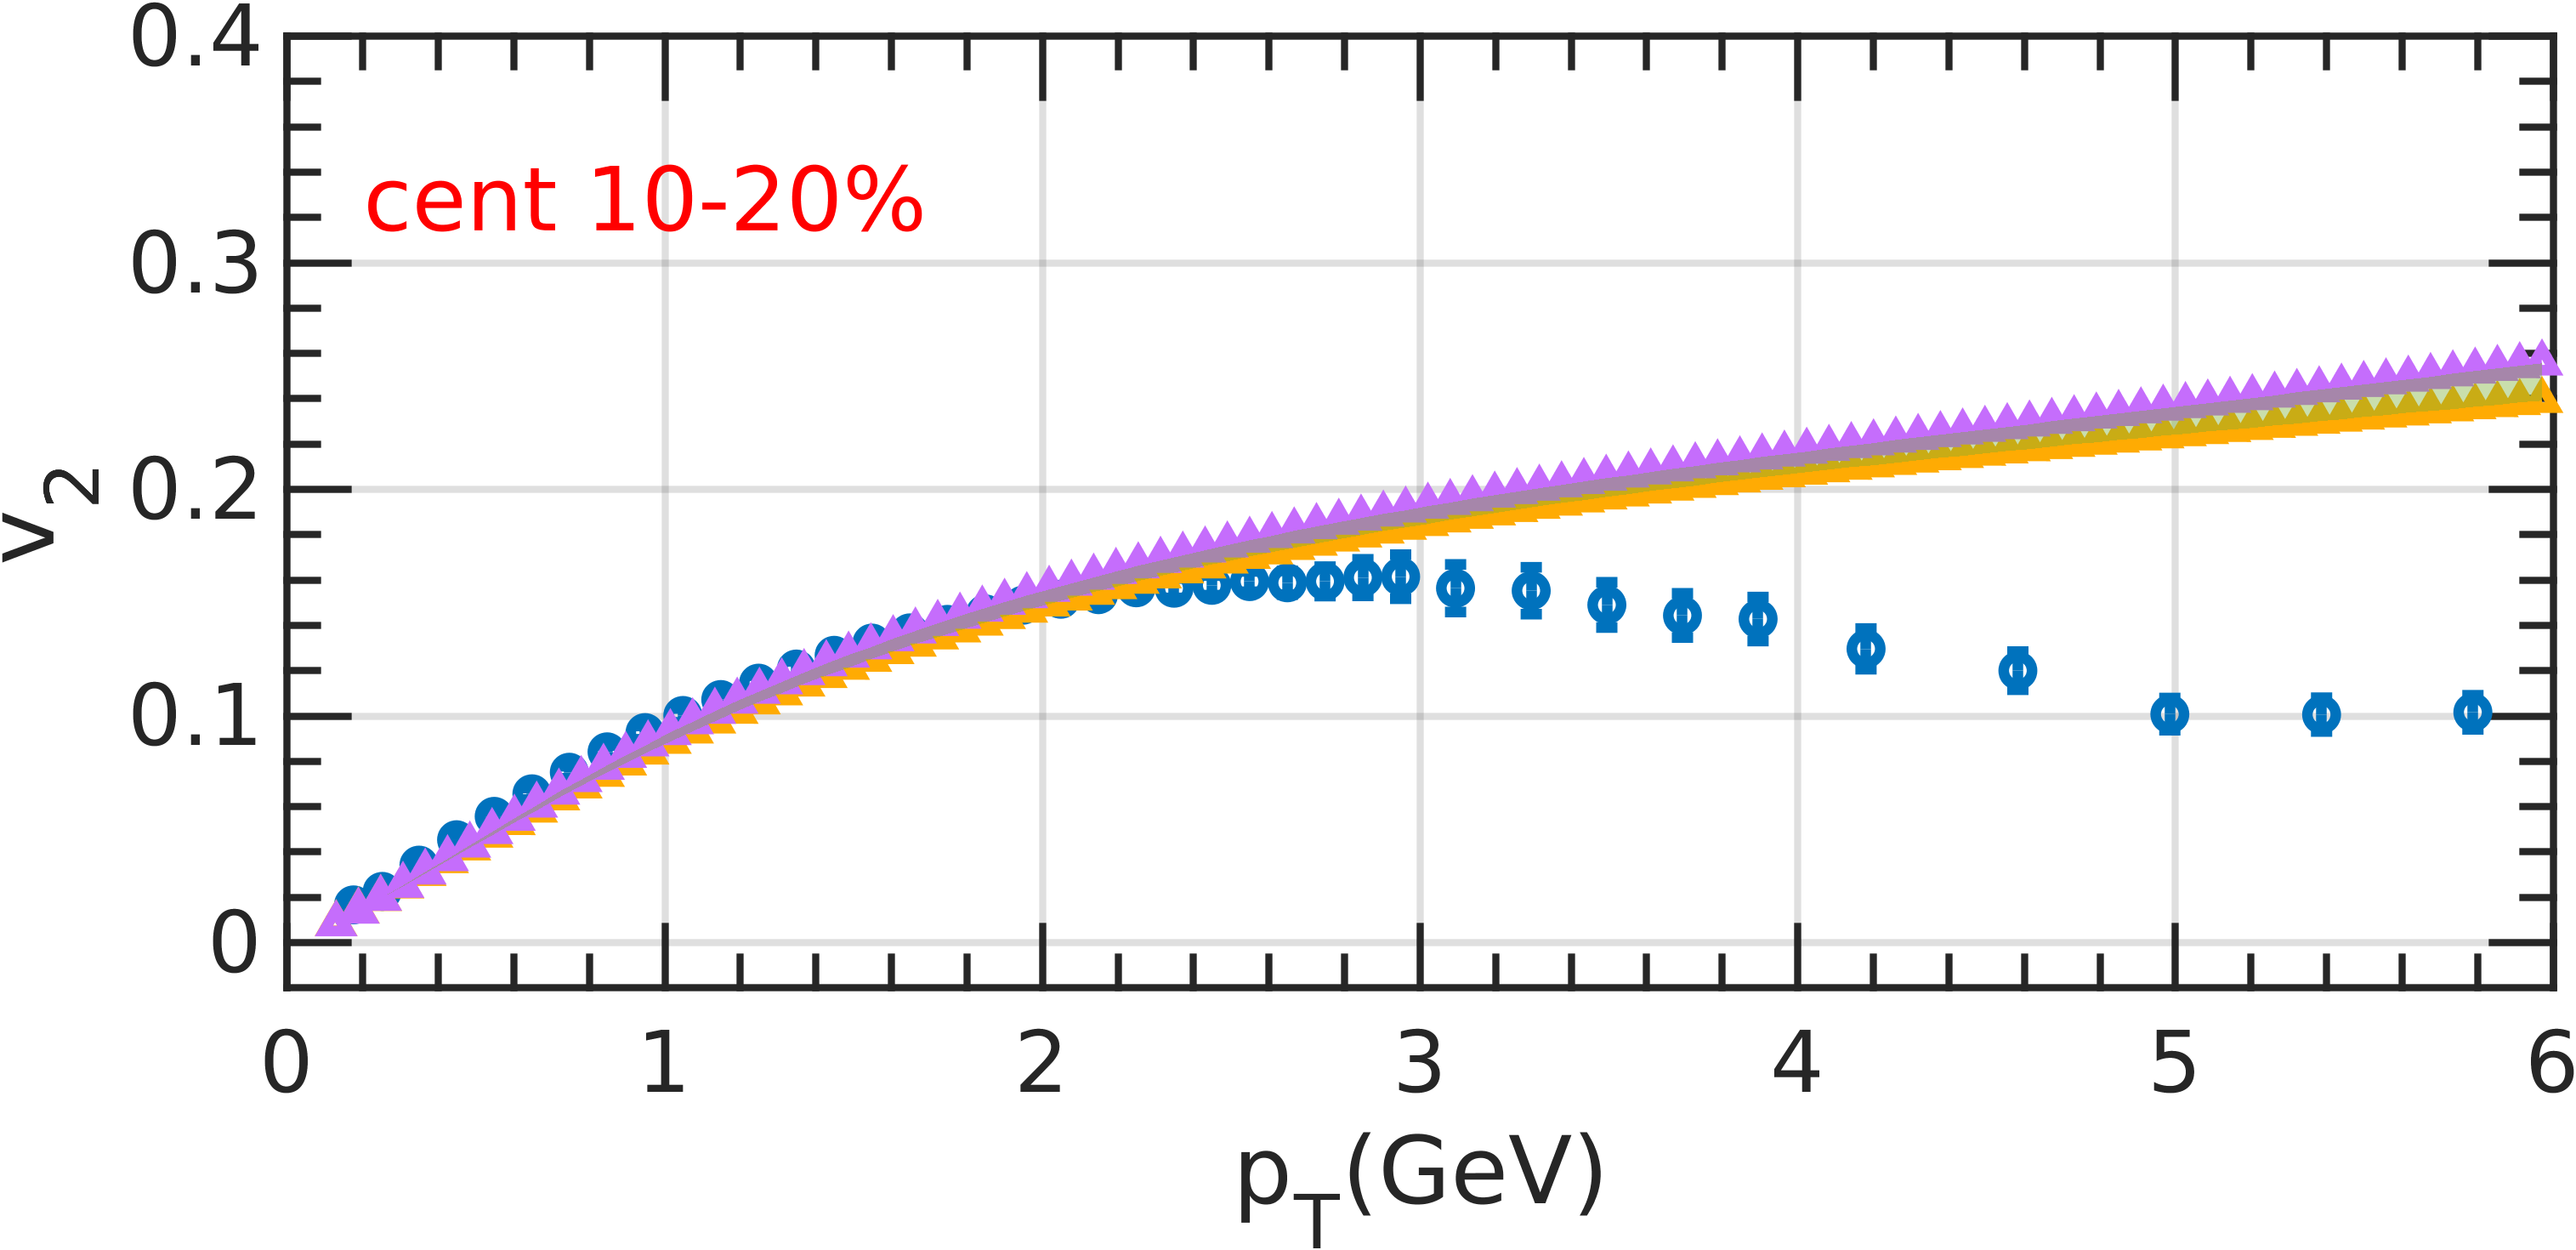
\includegraphics[scale=0.19]{figs/IPGlasma/v2_pT10-20.png}
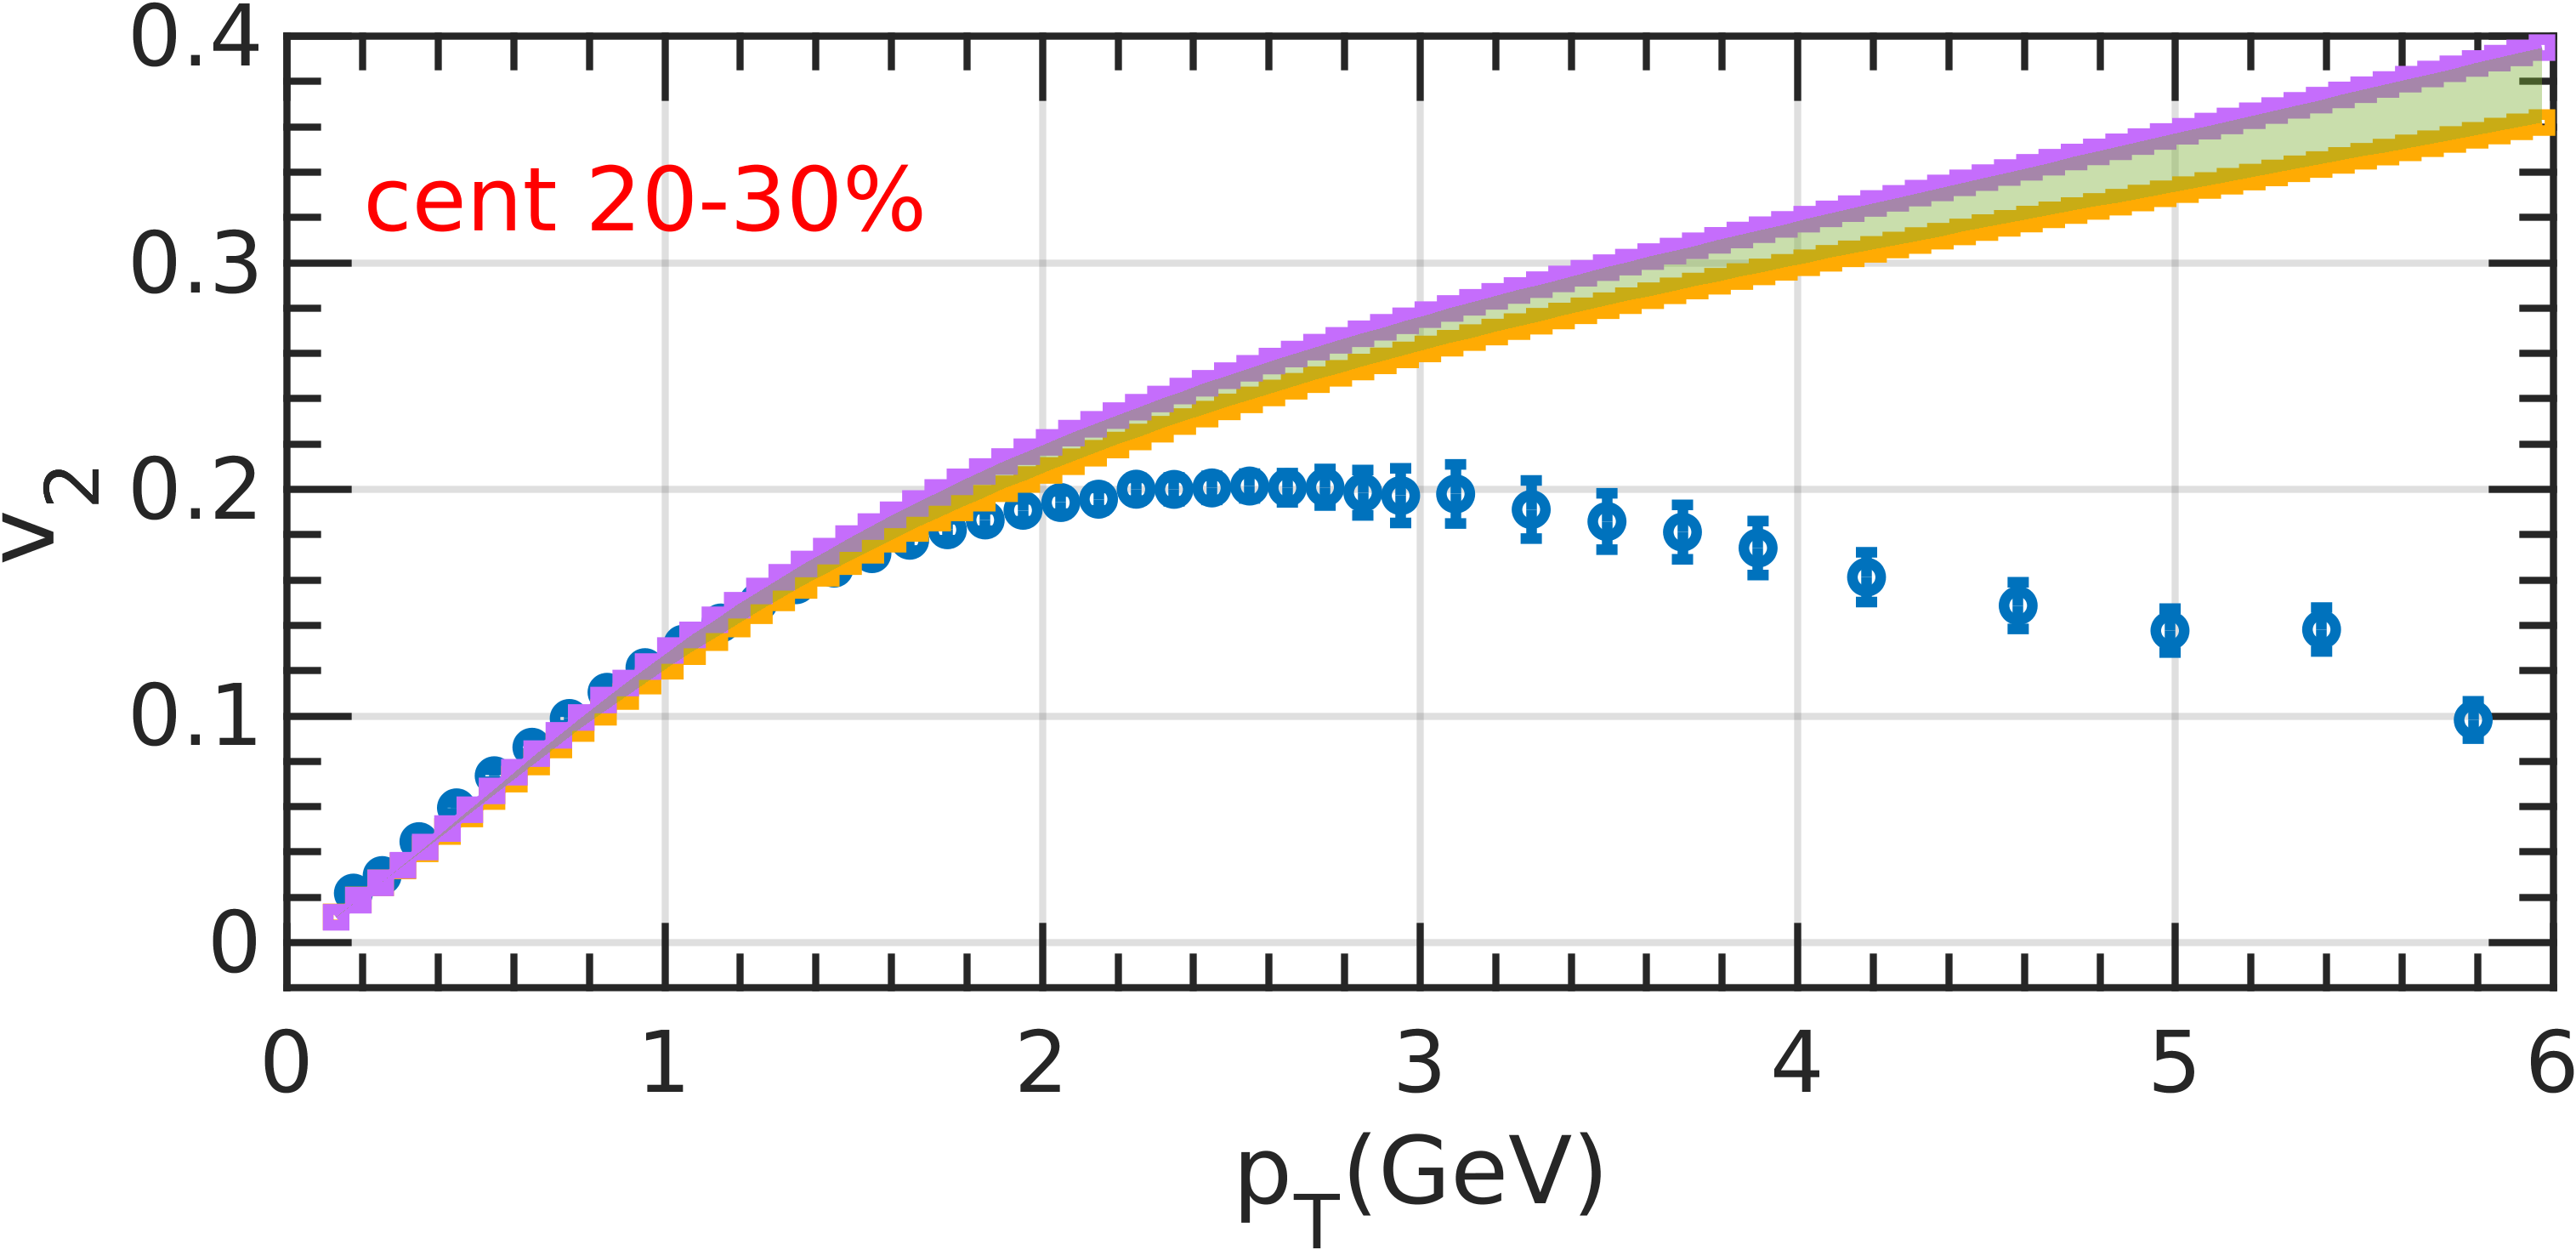
\includegraphics[scale=0.19]{figs/IPGlasma/v2_pT20-30.png}
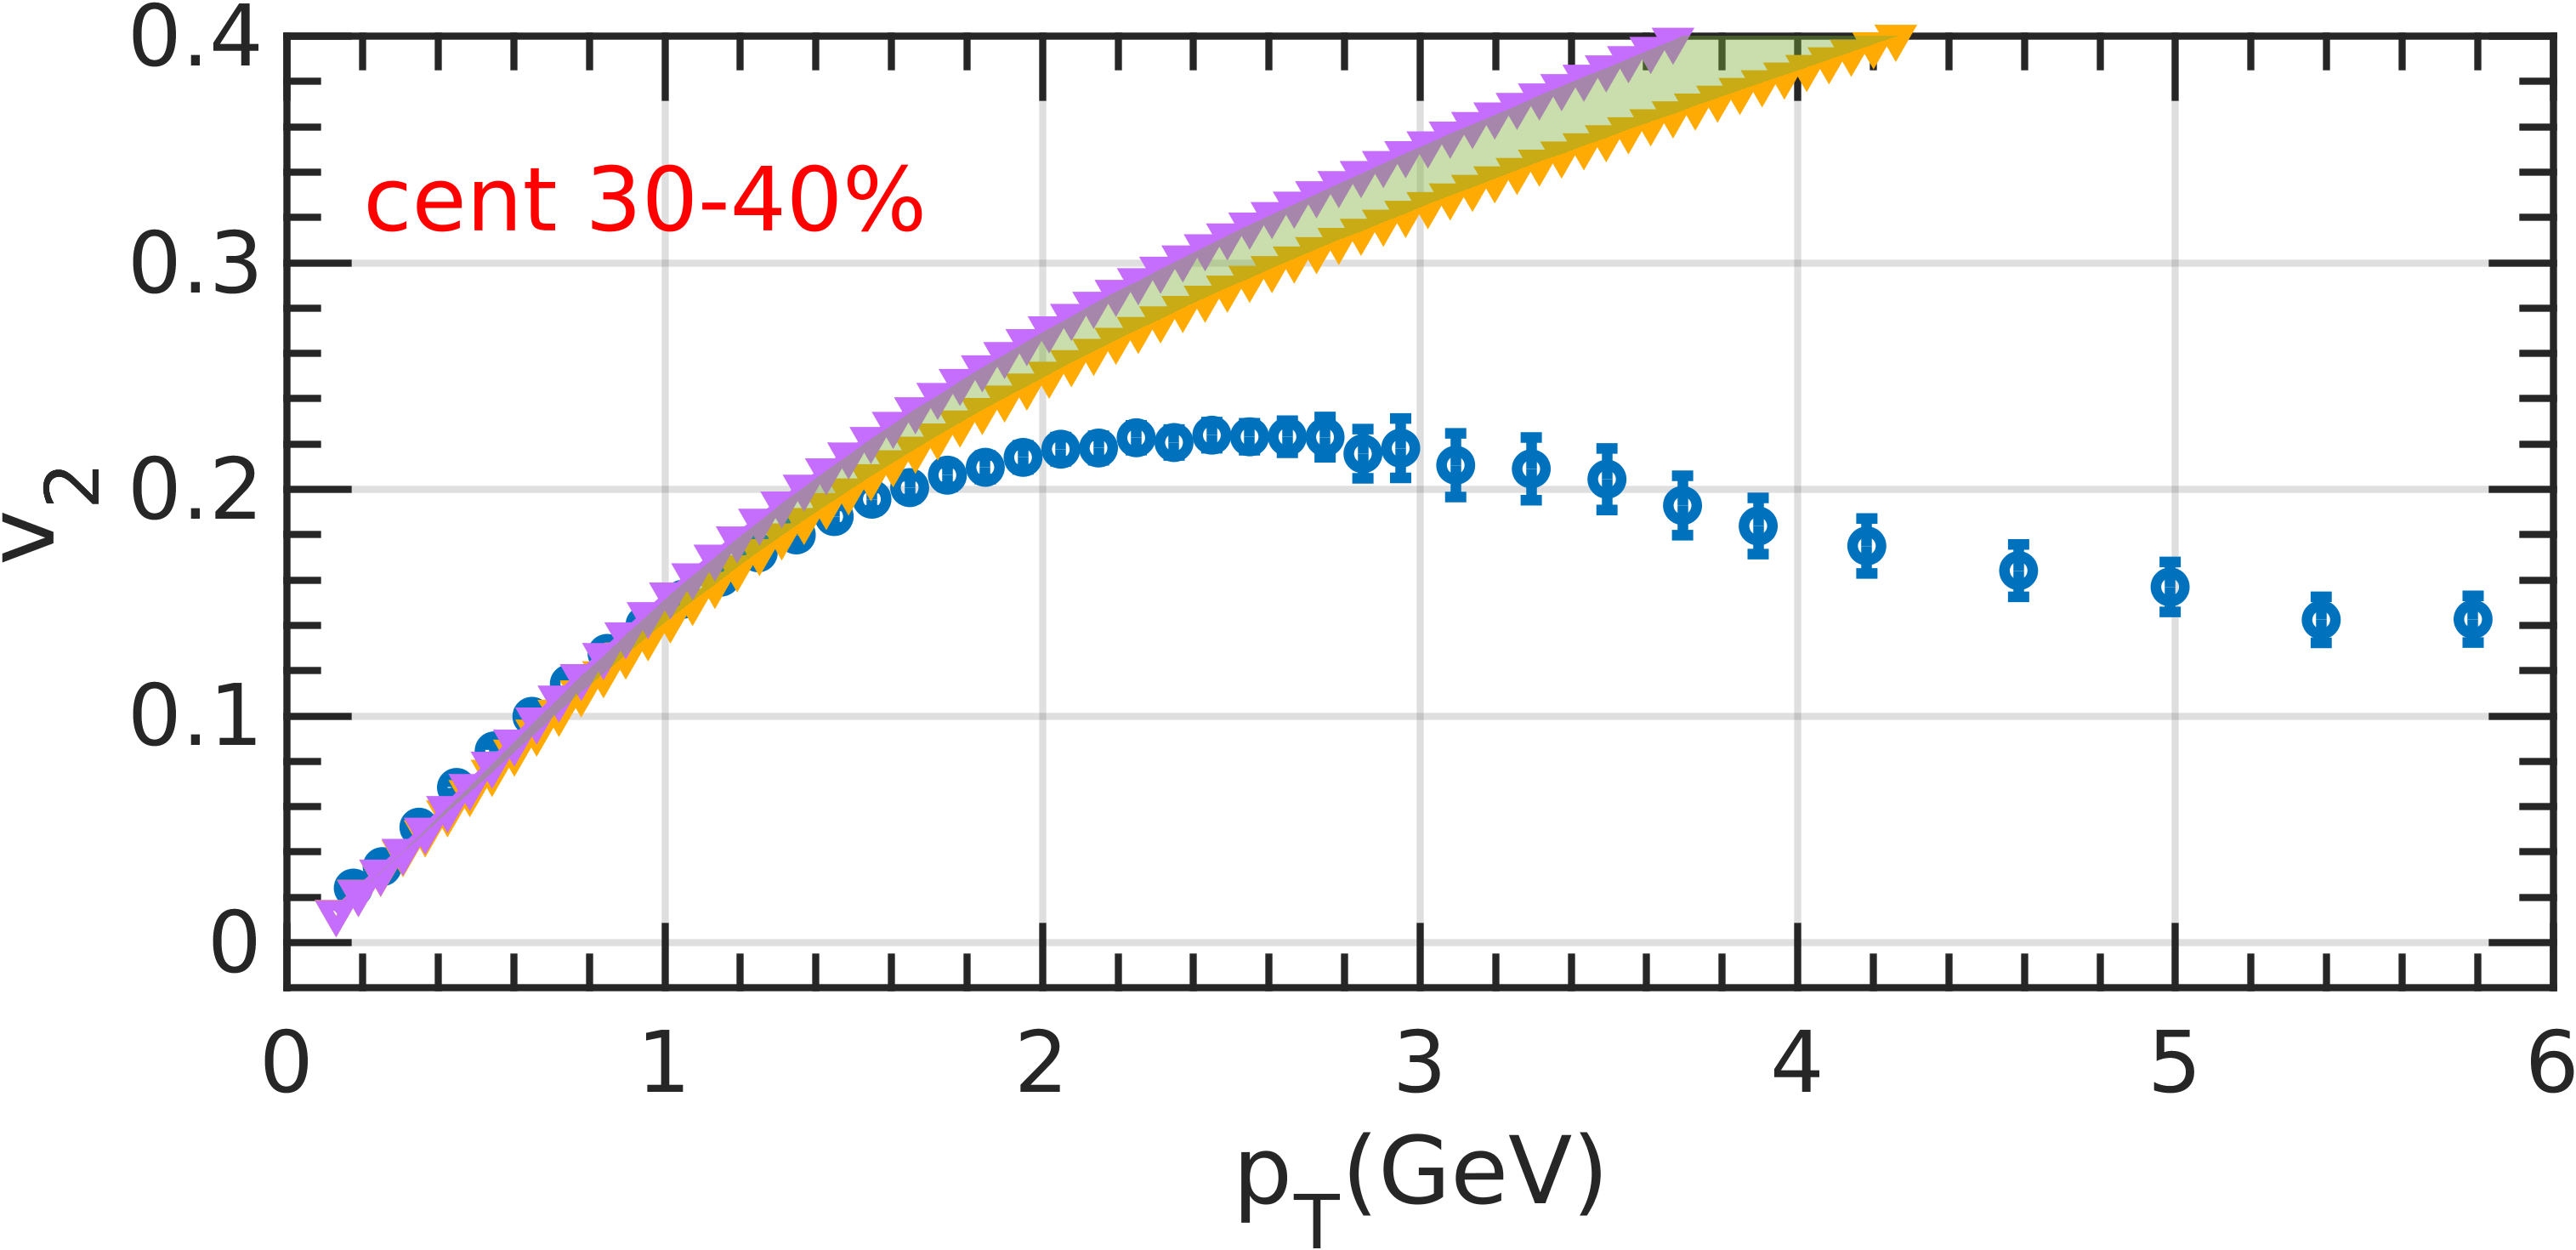
\includegraphics[scale=0.19]{figs/IPGlasma/v2_pT30-40.png}
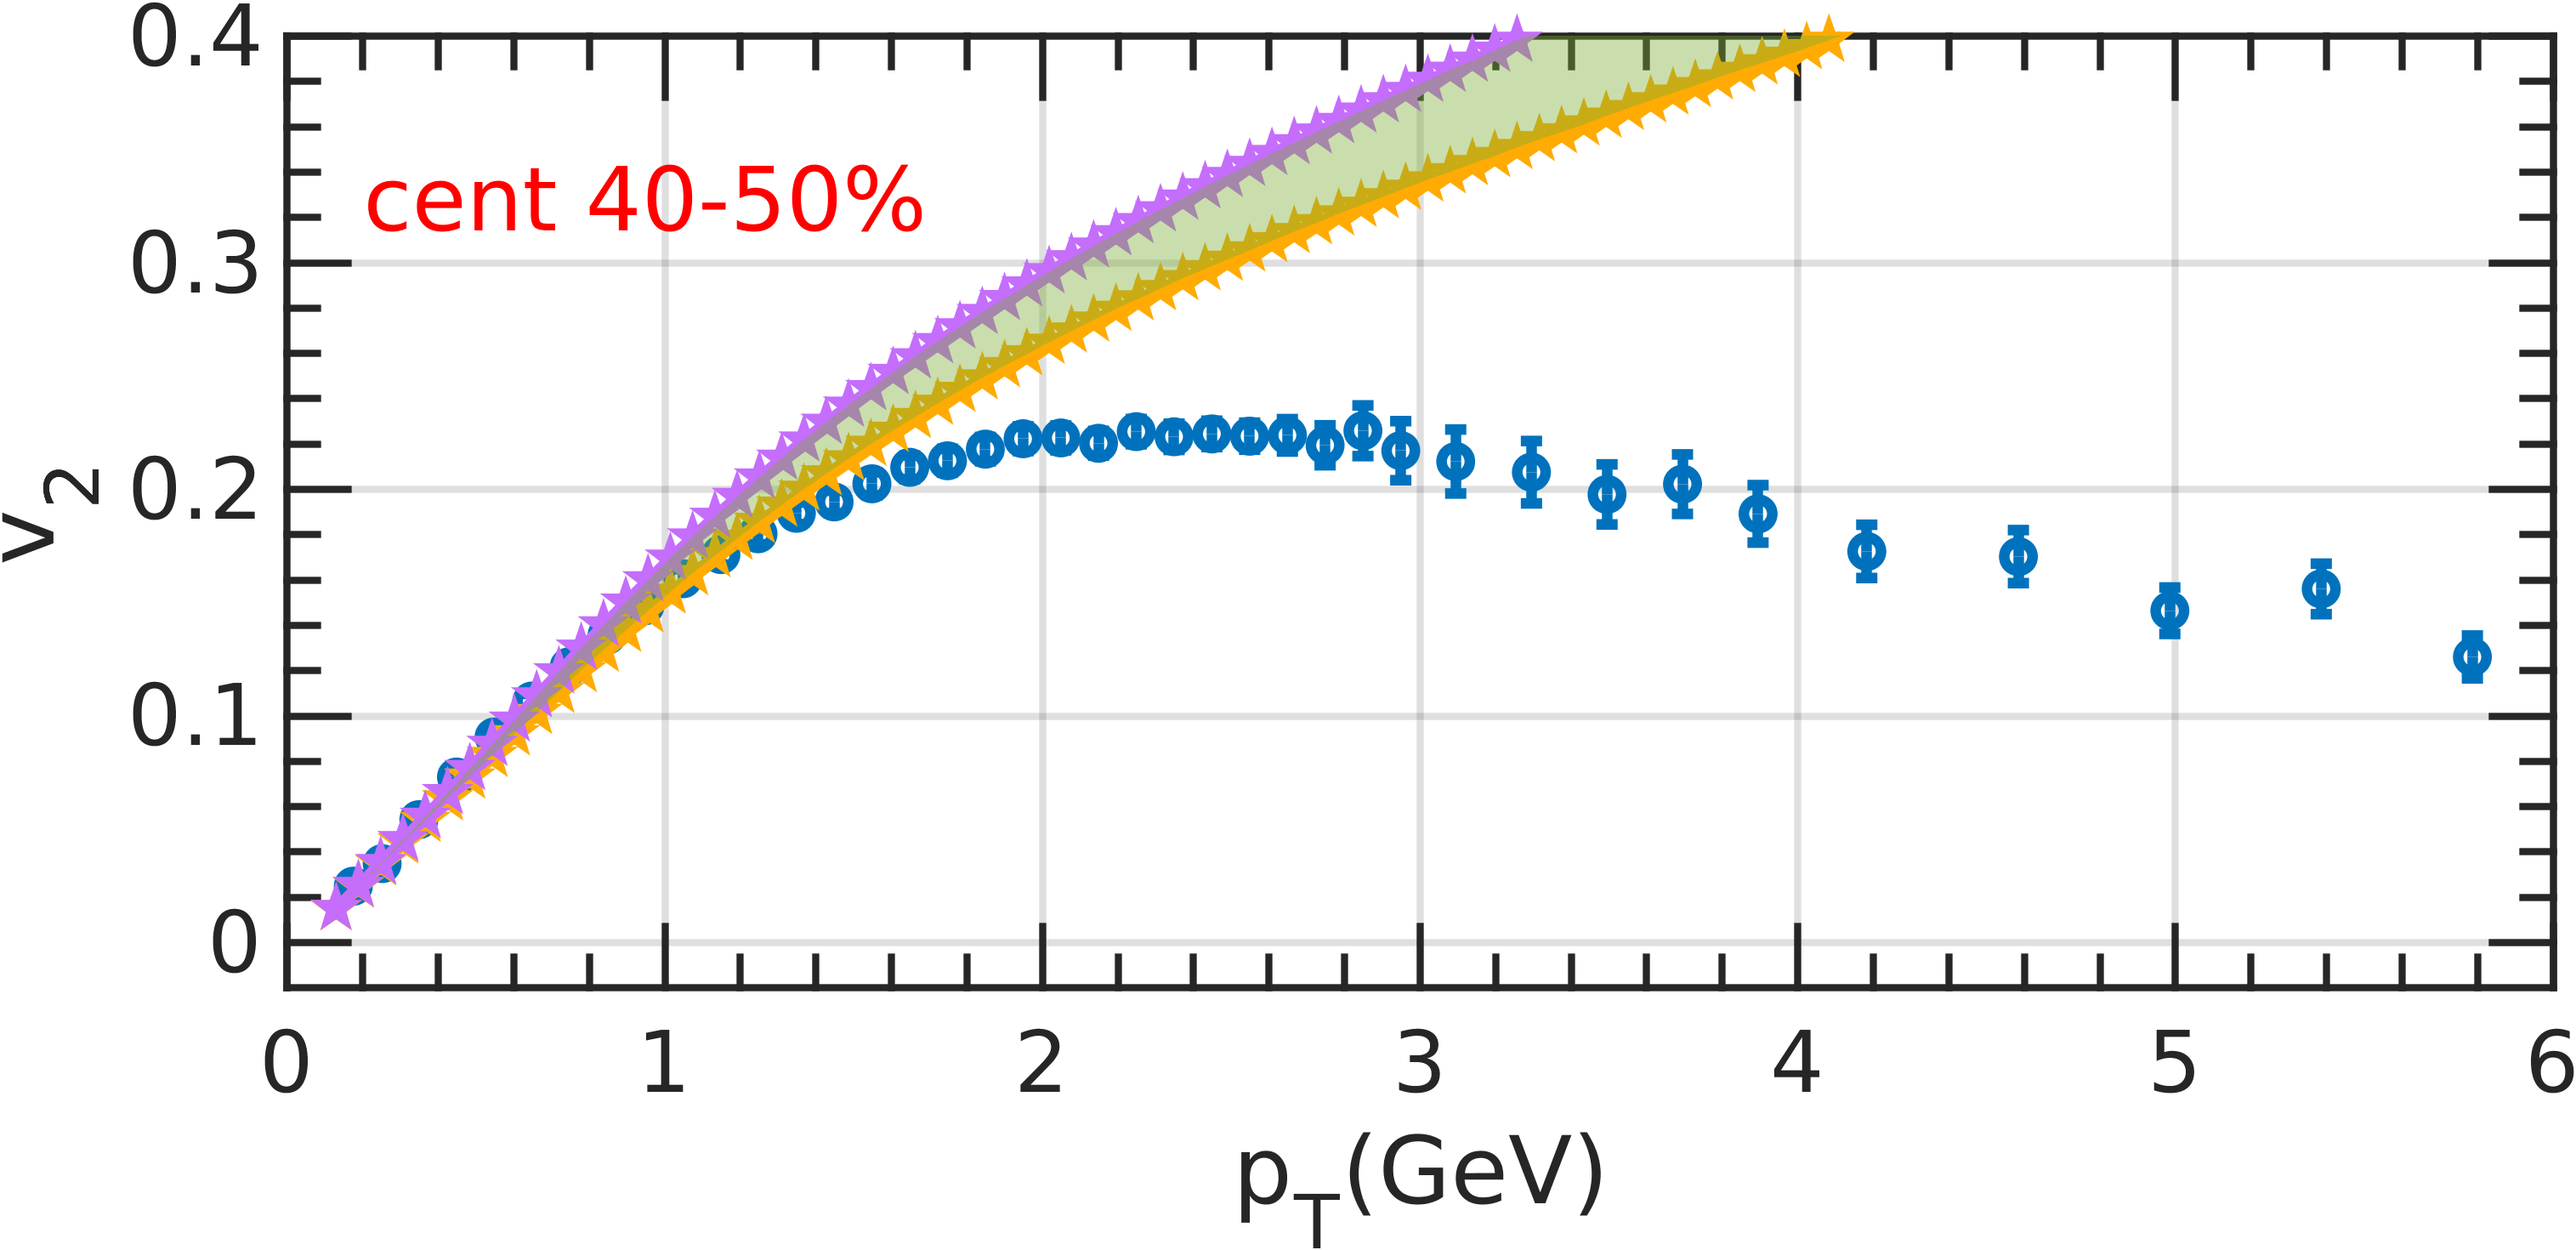
\includegraphics[scale=0.19]{figs/IPGlasma/v2_pT40-50.png}
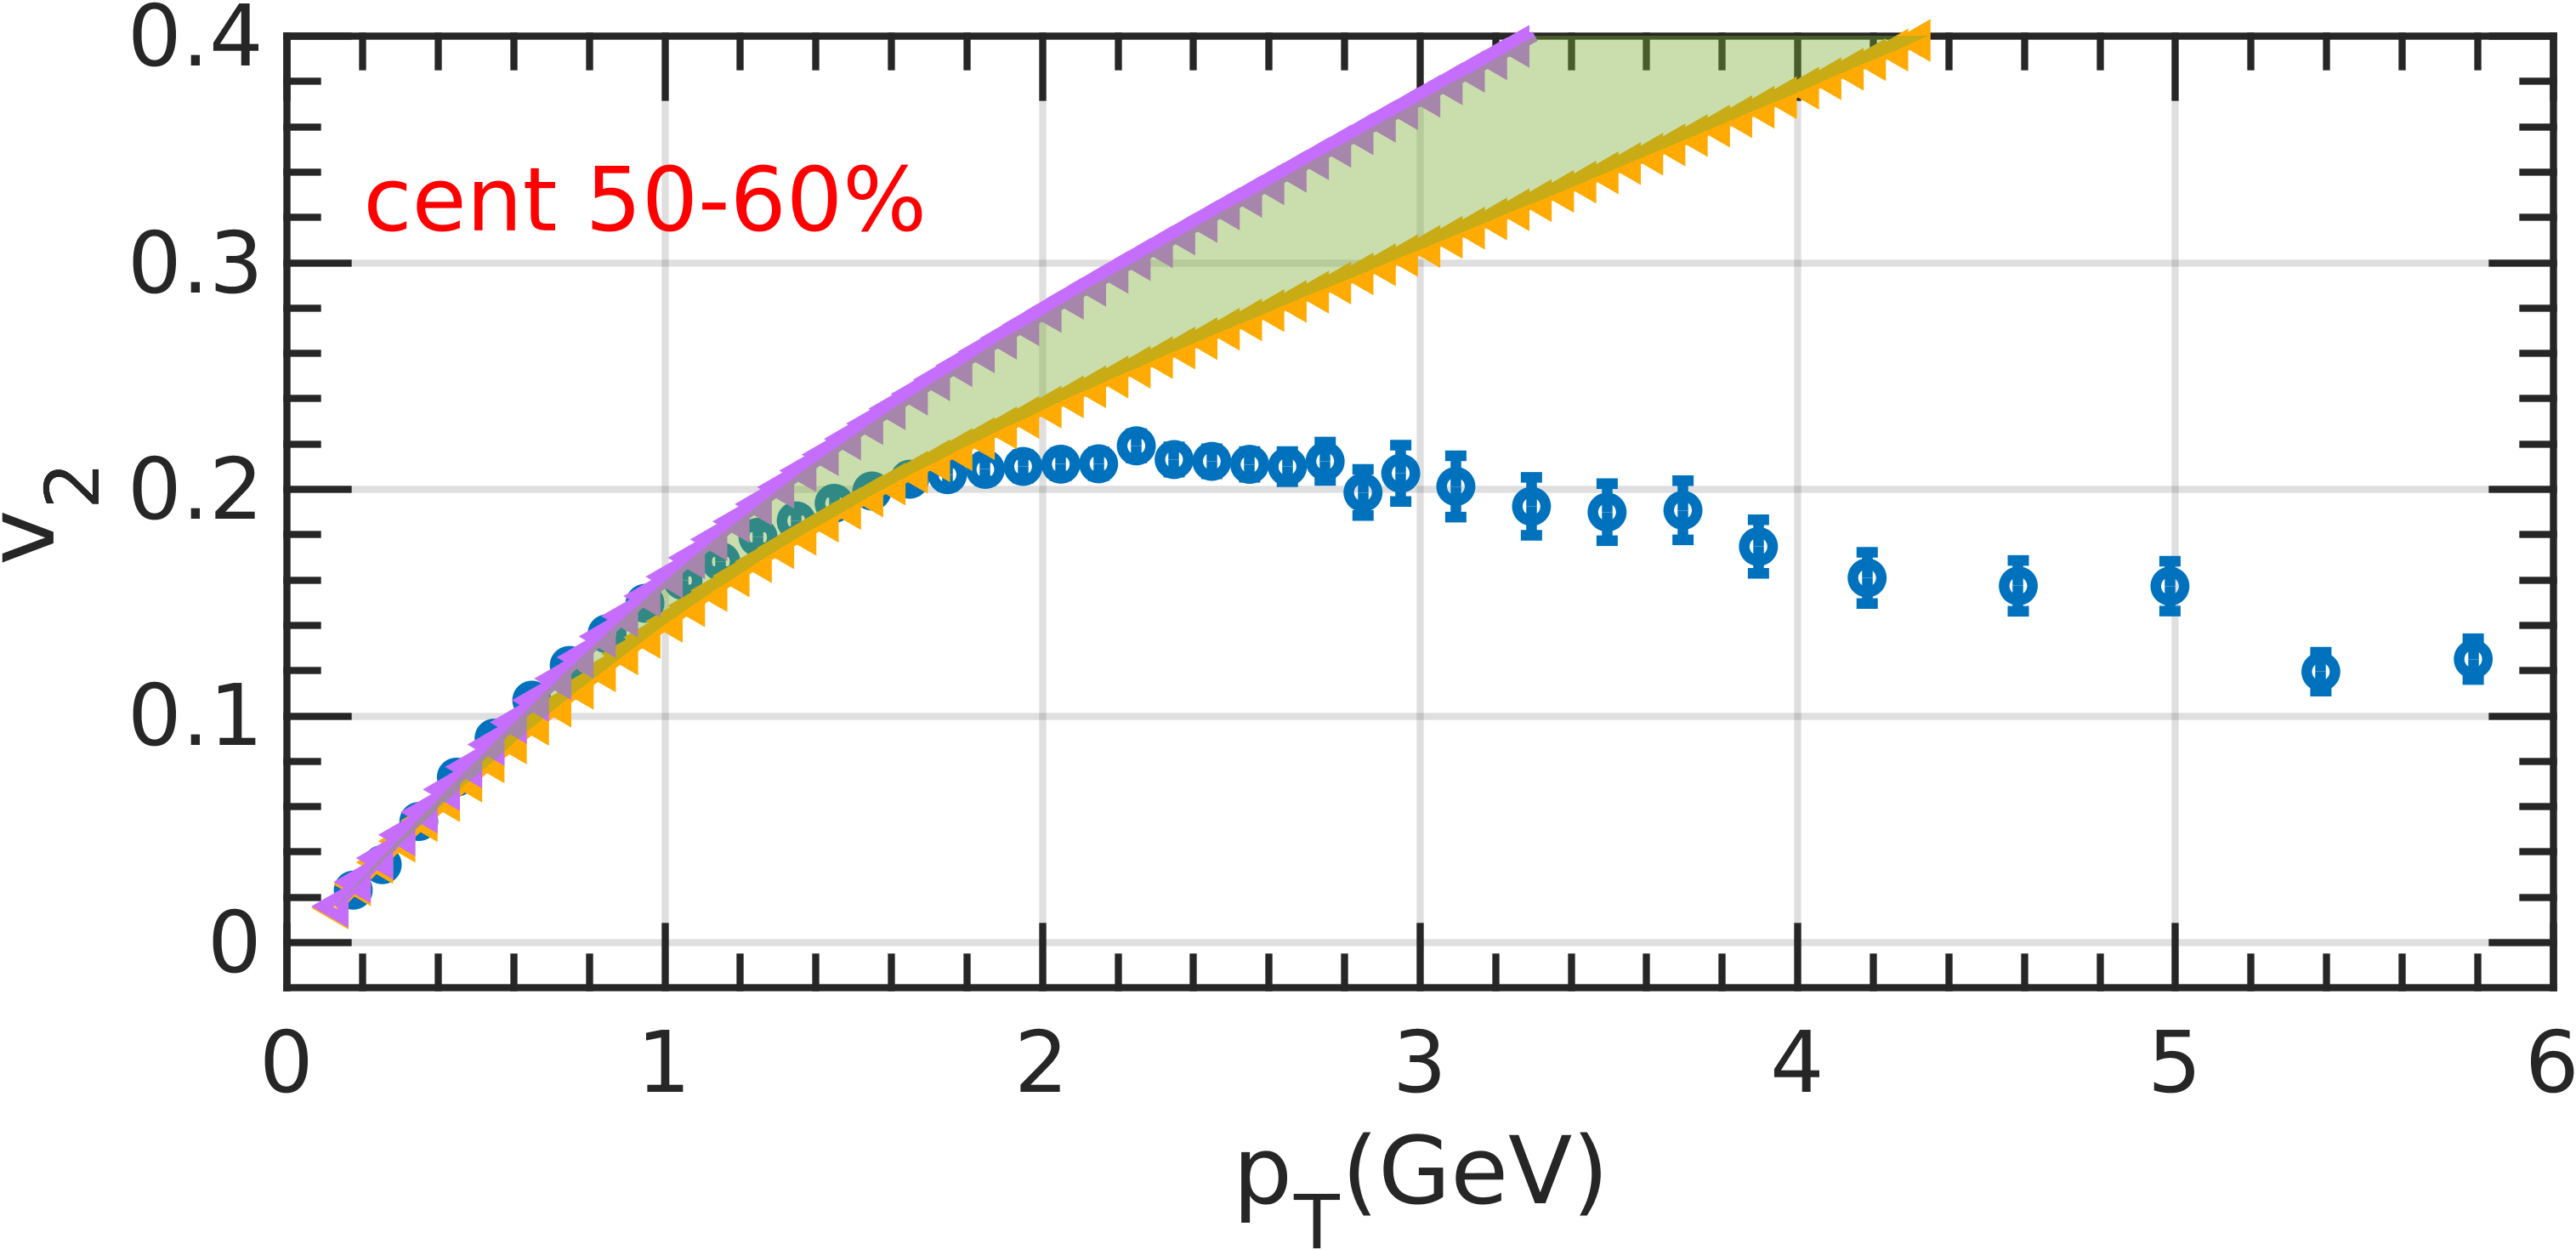
\includegraphics[scale=0.19]{figs/IPGlasma/v2_pT50-60.png}
%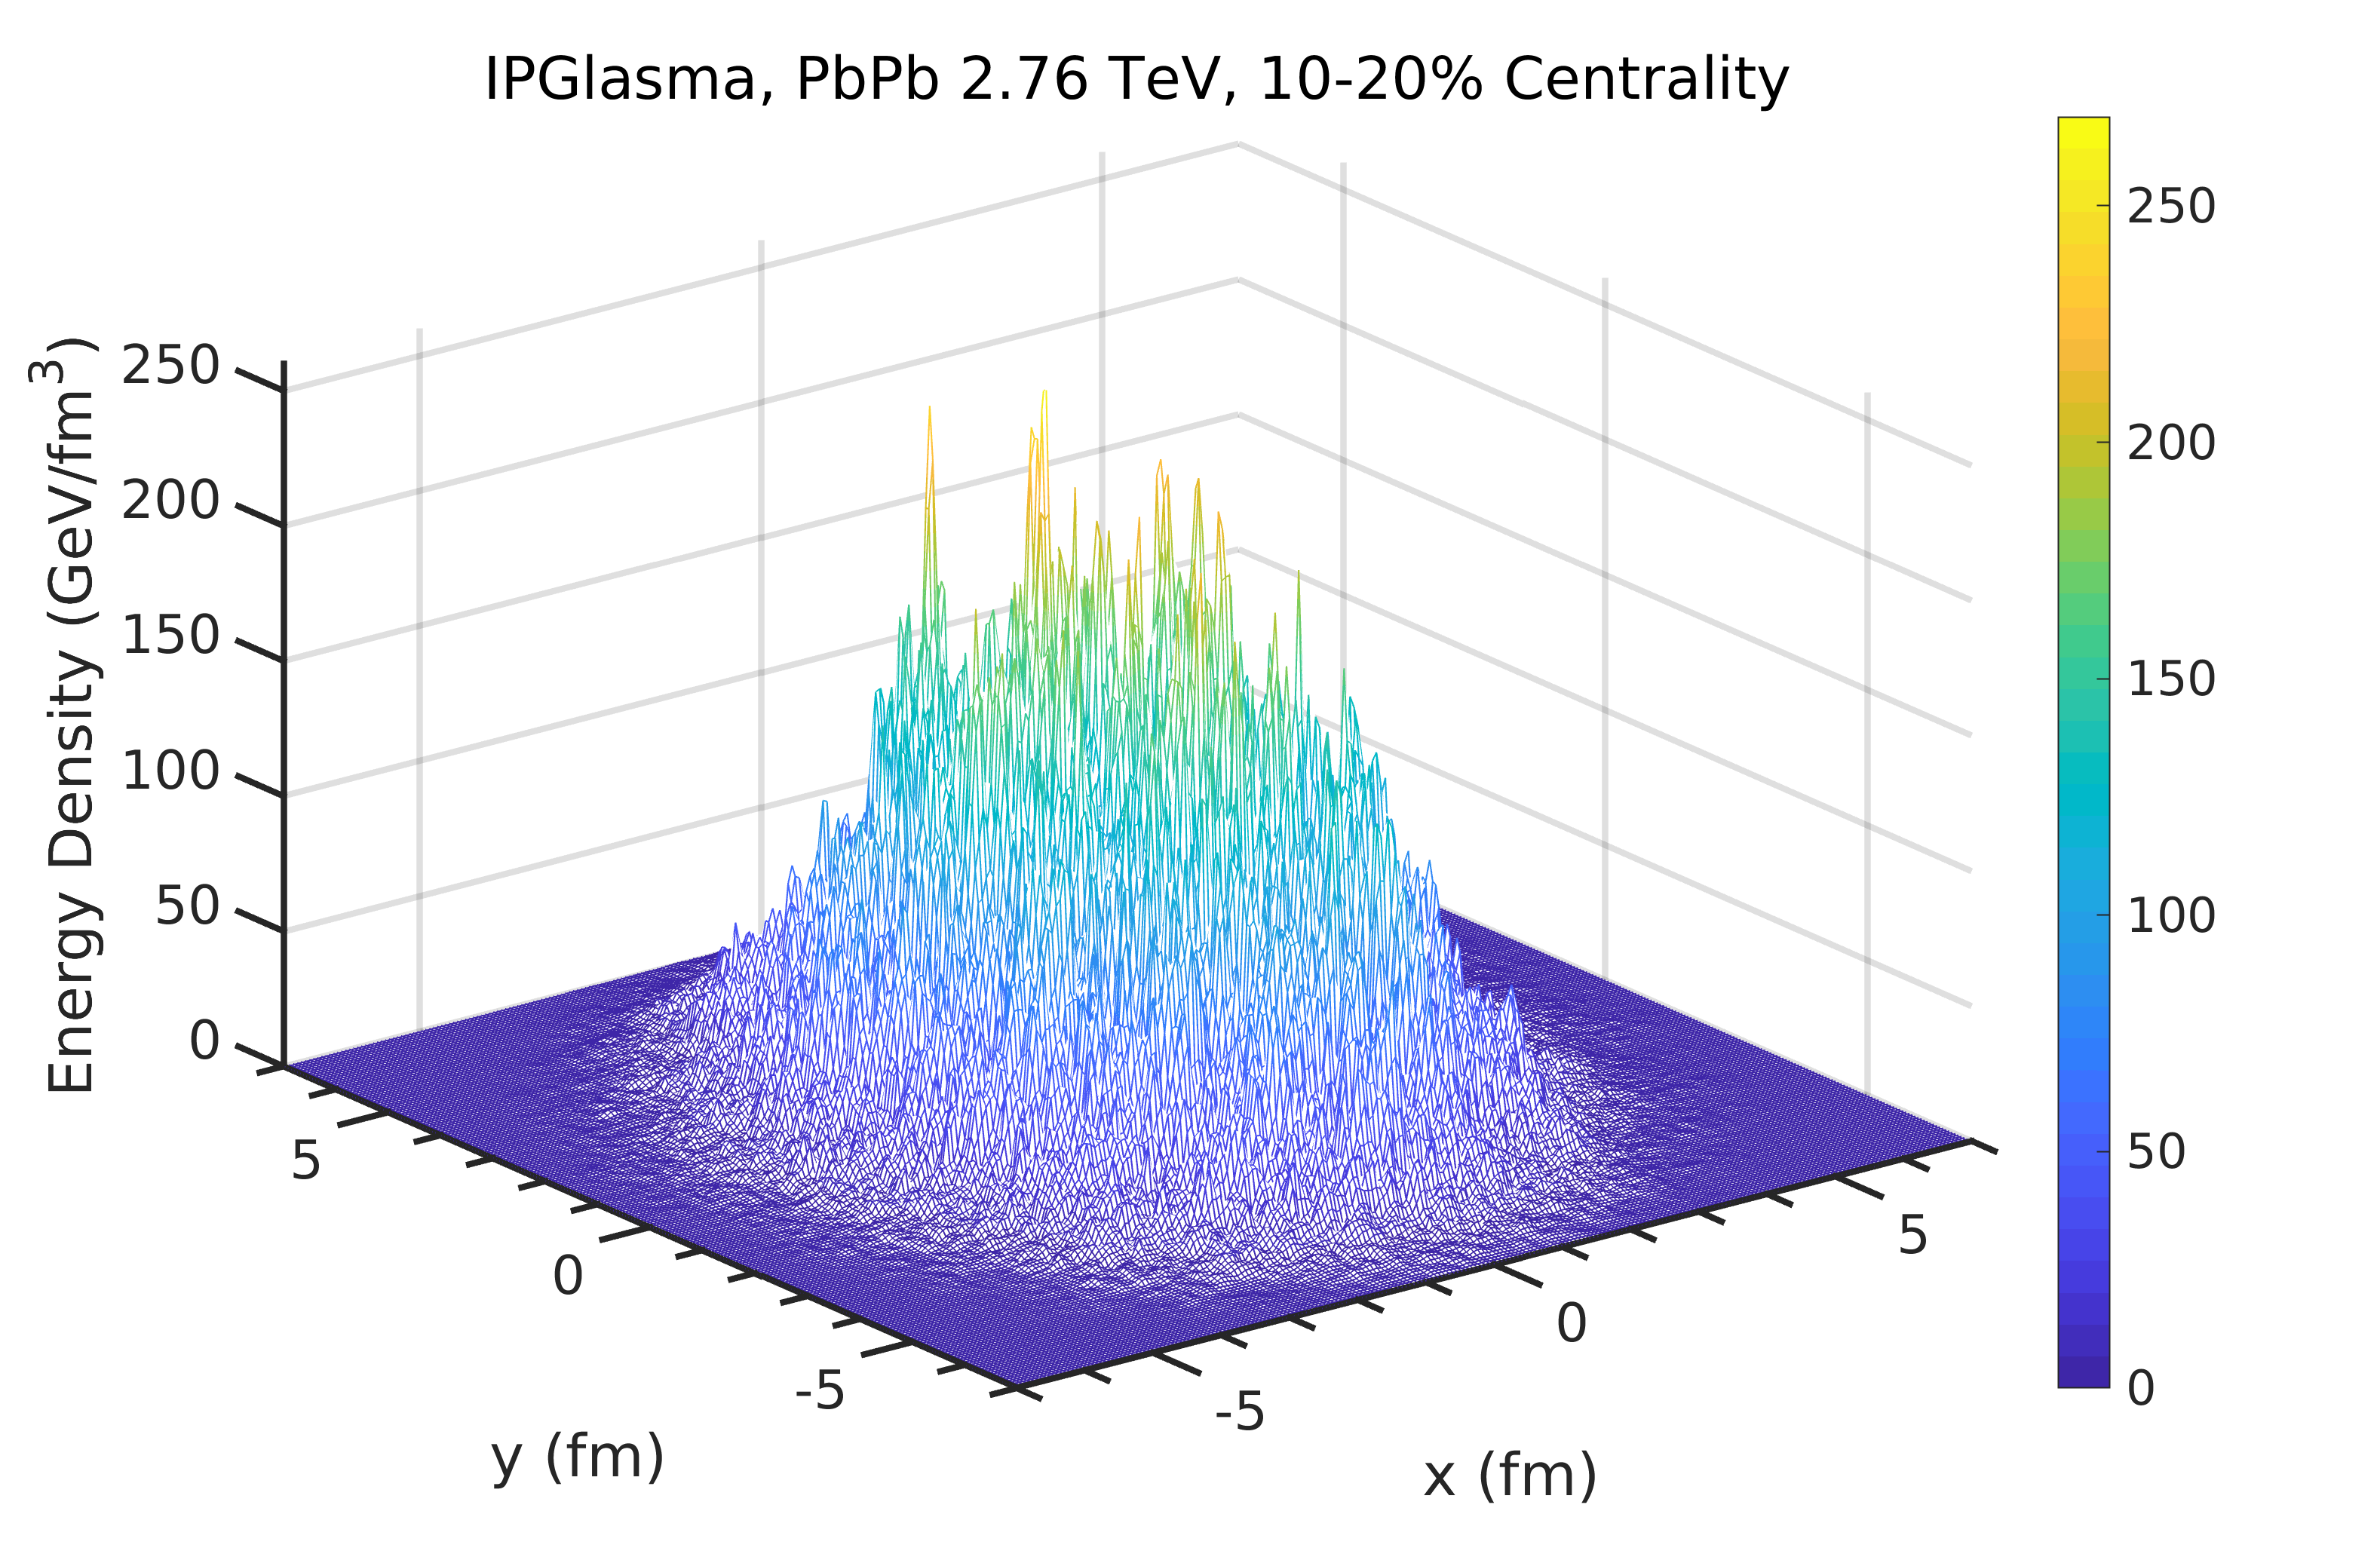
\includegraphics[scale=0.22]{figs/IPGlasma.png}
\end{figure}

\textit{J. High Energ. Phys. 2015, 190 (2015)}
\end{frame}



%------------------------------------------------


\begin{frame}
\frametitle{Elliptic flow vs $dN/d\eta$ plot}

\begin{figure}
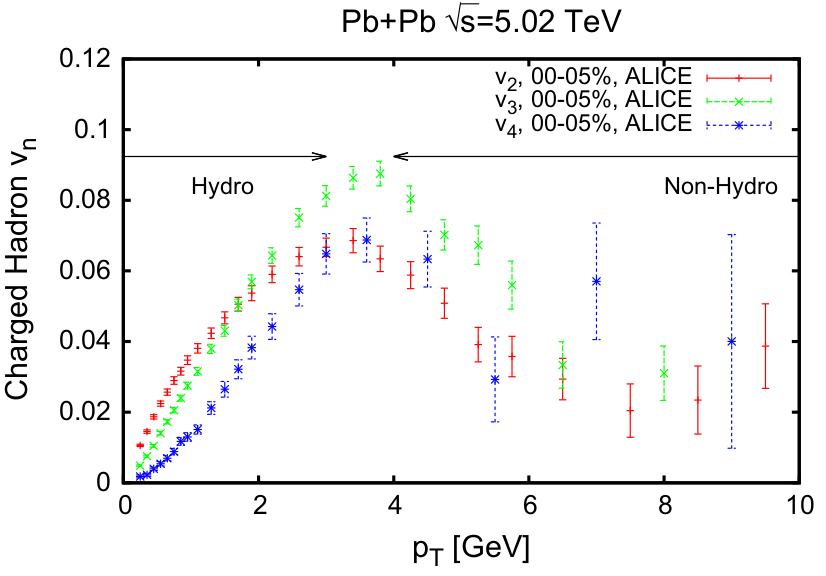
\includegraphics[scale=0.22]{figs/non_hydro.png}
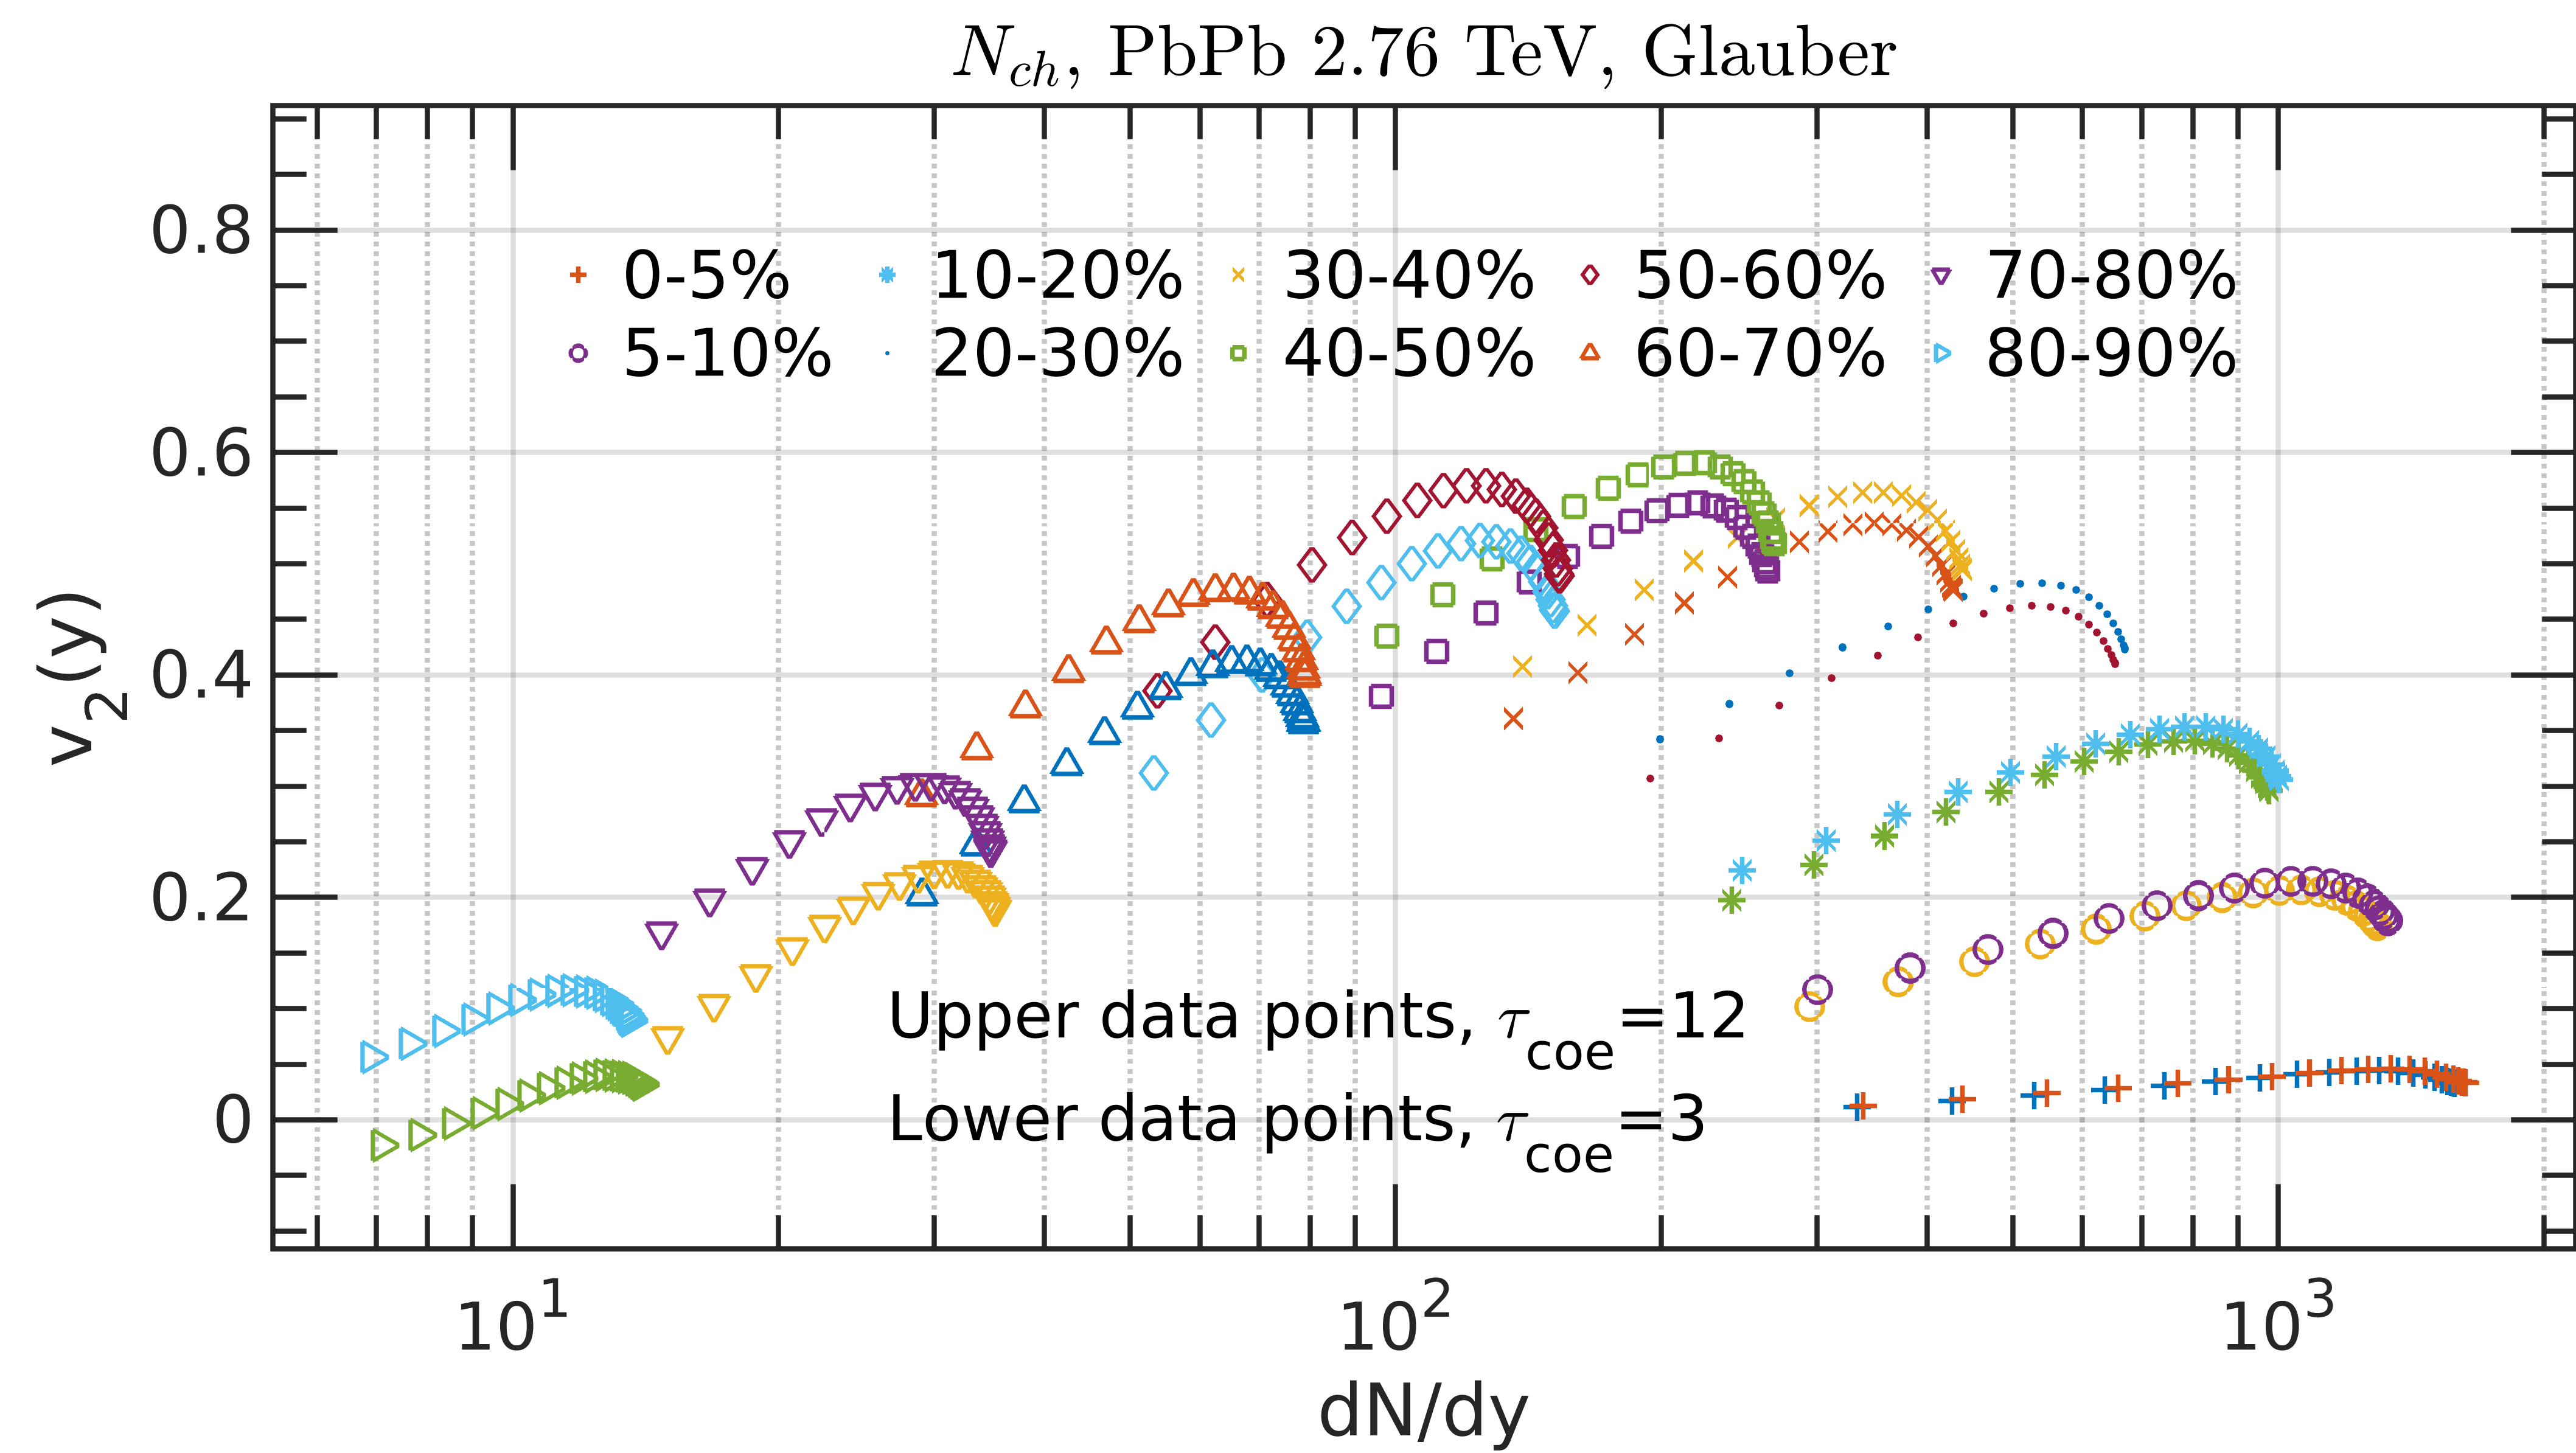
\includegraphics[scale=0.22]{figs/v2_dNdy_3Dgeometric.png}
\end{figure}

\begin{itemize}

\item P. Romatschke suggested that abrupt change in elliptic flow($v_2$) for variation in relaxation times at low multiplicity could potentially indicate breakdown of the hydrodynamics.

\item Low $p_T$ hydro regime where hydrodynamic results show agreement with data.\\~\\


 \textit{P. Romatschke, Eur. Phys. J C 77, 1 (2017)}
 
\end{itemize}
\end{frame}

%------------------------------------------------




\begin{frame}
\frametitle{Conclusion}

\begin{itemize}

 
\item Even the most peripheral PbPb, 2.76 TeV collisions are within the hydrodynamic regime. 

\item Large value of relaxation time leads to increase in elliptic flow for MIS hydrodynamic theory especially at high $p_T$.   

\item We see a larger flow increment in the Glauber model than in IPGlasma model. 

\item Elliptic flow in the most central collisions is not affected by the non-hydro mode structure of the
theory. For increasing impact parameter, the non-hydro mode participation also increases. 
Could we compare flow from different models at the most central collisions without worrying about non-hydro mode structure of the theory? caveat! 
% being the total flow itself is quite small in the most central collisions.)

\item Initial state fluctuations have a noticeable effect on the elliptic flow. 


\end{itemize}
\end{frame}


%------------------------------------------------

\begin{frame}
\Huge{\centerline{Thank you}}
\end{frame}

%----------------------------------------------------------------------------------------

\end{document}